% Options for packages loaded elsewhere
\PassOptionsToPackage{unicode}{hyperref}
\PassOptionsToPackage{hyphens}{url}
\PassOptionsToPackage{dvipsnames,svgnames,x11names}{xcolor}
%
\documentclass[
]{article}

\usepackage{amsmath,amssymb}
\usepackage{iftex}
\ifPDFTeX
  \usepackage[T1]{fontenc}
  \usepackage[utf8]{inputenc}
  \usepackage{textcomp} % provide euro and other symbols
\else % if luatex or xetex
  \usepackage{unicode-math}
  \defaultfontfeatures{Scale=MatchLowercase}
  \defaultfontfeatures[\rmfamily]{Ligatures=TeX,Scale=1}
\fi
\usepackage{lmodern}
\ifPDFTeX\else  
    % xetex/luatex font selection
    \setmainfont[]{Latin Modern Roman}
  \setmathfont[]{Latin Modern Math}
\fi
% Use upquote if available, for straight quotes in verbatim environments
\IfFileExists{upquote.sty}{\usepackage{upquote}}{}
\IfFileExists{microtype.sty}{% use microtype if available
  \usepackage[]{microtype}
  \UseMicrotypeSet[protrusion]{basicmath} % disable protrusion for tt fonts
}{}
\makeatletter
\@ifundefined{KOMAClassName}{% if non-KOMA class
  \IfFileExists{parskip.sty}{%
    \usepackage{parskip}
  }{% else
    \setlength{\parindent}{0pt}
    \setlength{\parskip}{6pt plus 2pt minus 1pt}}
}{% if KOMA class
  \KOMAoptions{parskip=half}}
\makeatother
\usepackage{xcolor}
\setlength{\emergencystretch}{3em} % prevent overfull lines
\setcounter{secnumdepth}{5}
% Make \paragraph and \subparagraph free-standing
\makeatletter
\ifx\paragraph\undefined\else
  \let\oldparagraph\paragraph
  \renewcommand{\paragraph}{
    \@ifstar
      \xxxParagraphStar
      \xxxParagraphNoStar
  }
  \newcommand{\xxxParagraphStar}[1]{\oldparagraph*{#1}\mbox{}}
  \newcommand{\xxxParagraphNoStar}[1]{\oldparagraph{#1}\mbox{}}
\fi
\ifx\subparagraph\undefined\else
  \let\oldsubparagraph\subparagraph
  \renewcommand{\subparagraph}{
    \@ifstar
      \xxxSubParagraphStar
      \xxxSubParagraphNoStar
  }
  \newcommand{\xxxSubParagraphStar}[1]{\oldsubparagraph*{#1}\mbox{}}
  \newcommand{\xxxSubParagraphNoStar}[1]{\oldsubparagraph{#1}\mbox{}}
\fi
\makeatother


\providecommand{\tightlist}{%
  \setlength{\itemsep}{0pt}\setlength{\parskip}{0pt}}\usepackage{longtable,booktabs,array}
\usepackage{calc} % for calculating minipage widths
% Correct order of tables after \paragraph or \subparagraph
\usepackage{etoolbox}
\makeatletter
\patchcmd\longtable{\par}{\if@noskipsec\mbox{}\fi\par}{}{}
\makeatother
% Allow footnotes in longtable head/foot
\IfFileExists{footnotehyper.sty}{\usepackage{footnotehyper}}{\usepackage{footnote}}
\makesavenoteenv{longtable}
\usepackage{graphicx}
\makeatletter
\newsavebox\pandoc@box
\newcommand*\pandocbounded[1]{% scales image to fit in text height/width
  \sbox\pandoc@box{#1}%
  \Gscale@div\@tempa{\textheight}{\dimexpr\ht\pandoc@box+\dp\pandoc@box\relax}%
  \Gscale@div\@tempb{\linewidth}{\wd\pandoc@box}%
  \ifdim\@tempb\p@<\@tempa\p@\let\@tempa\@tempb\fi% select the smaller of both
  \ifdim\@tempa\p@<\p@\scalebox{\@tempa}{\usebox\pandoc@box}%
  \else\usebox{\pandoc@box}%
  \fi%
}
% Set default figure placement to htbp
\def\fps@figure{htbp}
\makeatother

\usepackage{pdflscape}
\usepackage{fancyhdr}
\usepackage{lscape}
\usepackage{pdflscape}
\usepackage{fancyhdr}
\usepackage{gensymb}

% Redefine landscape commands for easier use
\newcommand{\blandscape}{\begin{landscape}}
\newcommand{\elandscape}{\end{landscape}}

% Custom page style for landscape pages
\fancypagestyle{landscape}{%
  \fancyhf{} % Clear all header and footer fields
  \fancyfoot[C]{\thepage} % Center page number on long edge
  \renewcommand{\headrulewidth}{0pt}
  \renewcommand{\footrulewidth}{0pt}
}

% Hook into the landscape environment
\AtBeginEnvironment{landscape}{\pagestyle{landscape}}
\usepackage{booktabs}
\usepackage{caption}
\usepackage{longtable}
\usepackage{colortbl}
\usepackage{array}
\usepackage{anyfontsize}
\usepackage{multirow}
\usepackage{arxiv}
\usepackage{orcidlink}
\usepackage{amsmath}
\usepackage[T1]{fontenc}
\makeatletter
\@ifpackageloaded{float}{}{\usepackage{float}}
\floatstyle{plain}
\@ifundefined{c@chapter}{\newfloat{fig}{h}{lofig}}{\newfloat{fig}{h}{lofig}[chapter]}
\floatname{fig}{Figure}
\newcommand*\listoffigs{\listof{fig}{List of Figures}}
\makeatother
\makeatletter
\@ifpackageloaded{float}{}{\usepackage{float}}
\floatstyle{plain}
\@ifundefined{c@chapter}{\newfloat{suppfig}{h}{losuppfig}}{\newfloat{suppfig}{h}{losuppfig}[chapter]}
\floatname{suppfig}{Supplementary Figure}
\newcommand*\listofsuppfigs{\listof{suppfig}{List of Supplementary Figures}}
\makeatother
\makeatletter
\@ifpackageloaded{float}{}{\usepackage{float}}
\floatstyle{plain}
\@ifundefined{c@chapter}{\newfloat{tbl}{h}{lotbl}}{\newfloat{tbl}{h}{lotbl}[chapter]}
\floatname{tbl}{Table}
\newcommand*\listoftbls{\listof{tbl}{List of Tables}}
\makeatother
\makeatletter
\@ifpackageloaded{float}{}{\usepackage{float}}
\floatstyle{plain}
\@ifundefined{c@chapter}{\newfloat{supptbl}{h}{losupptbl}}{\newfloat{supptbl}{h}{losupptbl}[chapter]}
\floatname{supptbl}{Supplementary Table}
\newcommand*\listofsupptbls{\listof{supptbl}{List of Supplementary Tables}}
\makeatother
\makeatletter
\@ifpackageloaded{caption}{}{\usepackage{caption}}
\AtBeginDocument{%
\ifdefined\contentsname
  \renewcommand*\contentsname{Table of contents}
\else
  \newcommand\contentsname{Table of contents}
\fi
\ifdefined\listfigurename
  \renewcommand*\listfigurename{List of Figures}
\else
  \newcommand\listfigurename{List of Figures}
\fi
\ifdefined\listtablename
  \renewcommand*\listtablename{List of Tables}
\else
  \newcommand\listtablename{List of Tables}
\fi
\ifdefined\figurename
  \renewcommand*\figurename{Figure}
\else
  \newcommand\figurename{Figure}
\fi
\ifdefined\tablename
  \renewcommand*\tablename{Table}
\else
  \newcommand\tablename{Table}
\fi
}
\@ifpackageloaded{float}{}{\usepackage{float}}
\floatstyle{ruled}
\@ifundefined{c@chapter}{\newfloat{codelisting}{h}{lop}}{\newfloat{codelisting}{h}{lop}[chapter]}
\floatname{codelisting}{Listing}
\newcommand*\listoflistings{\listof{codelisting}{List of Listings}}
\makeatother
\makeatletter
\makeatother
\makeatletter
\@ifpackageloaded{caption}{}{\usepackage{caption}}
\@ifpackageloaded{subcaption}{}{\usepackage{subcaption}}
\makeatother

\usepackage[]{natbib}
\bibliographystyle{plainnat}
\usepackage{bookmark}

\IfFileExists{xurl.sty}{\usepackage{xurl}}{} % add URL line breaks if available
\urlstyle{same} % disable monospaced font for URLs
\hypersetup{
  pdftitle={Exploring Nutrient Availability and Herbivorous Insect Population Dynamics Across Multiple Scales},
  pdfkeywords={nitrogen, phosphorus, grasshoppers, population
dynamics, non-linear modeling, nutrient limitation, remote sensing},
  colorlinks=true,
  linkcolor={blue},
  filecolor={Maroon},
  citecolor={Blue},
  urlcolor={Blue},
  pdfcreator={LaTeX via pandoc}}


\usepackage{lineno}
\linenumbers
\renewcommand{\today}{2025-01-28}
\newcommand{\runninghead}{A Preprint }
\renewcommand{\runninghead}{initial submission }
\title{Exploring Nutrient Availability and Herbivorous Insect Population
Dynamics Across Multiple Scales}
\def\asep{\\\\\\ } % default: all authors on same column
\def\asep{\And }
\author{\asep\asep\asep\asep\asep\asep\asep\asep\asep}
\date{2025-01-28}
\begin{document}
\maketitle
\begin{abstract}
Nutrient composition varies greatly across landscapes, influencing the
spatiotemporal dynamics of populations. However, few studies have
explored this pattern across multiple scales. We tested how nutrient
limitation affects herbivore populations, from individual behavior to
landscape-level dynamics, using the Australian plague locust,
\emph{Chortoicetes terminifera} (Walker). Our study combined field
populations and long-term survey data across their range. At the
individual level, juvenile locusts selected a carbohydrate-biased intake
target of 1 protein (p) to 2 carbohydrate (c) and exhibited the highest
growth rates and shortest development times when fed artificial diets
matching this 1p:2c ratio during their final juvenile instar. In the
field, locusts exposed to protein-biased plants corrected their
nutritional imbalance by initially selecting carbohydrate-heavy diets
(up to a 1p:20c ratio). Over a week after removal from the protein-rich
environment, they returned to the 1p:2c intake target once the
deficiency was balanced. At the landscape level, locust outbreaks were
negatively correlated with soil nitrogen and exhibited a non-linear
relationship with soil phosphorus, peaking at approximately 4\%
phosphorus content. By disentangling the interaction between mean annual
precipitation and soil nitrogen, using comprehensive locust surveys and
remotely sensed soil and weather data spanning decades, we show how
environmental factors drive population dynamics. This study integrates
lab, field, and remote sensing approaches, highlighting the importance
of nutrient balancing across scales for herbivores. Specifically, we
demonstrate that low-nitrogen environments promote locust outbreaks,
likely by reducing plant protein-to-carbohydrate ratios. Incorporating
soil quality data into locust plague forecasting models could
significantly improve prediction accuracy.
\end{abstract}
{\bfseries \emph Keywords}
\def\sep{\textbullet\ }
nitrogen \sep phosphorus \sep grasshoppers \sep population
dynamics \sep non-linear modeling \sep nutrient limitation \sep 
remote sensing



\section{INTRODUCTION}\label{introduction}

Plant nutrients are usually more variable than animal body composition
both in their total amounts and ratios, which can make it challenging
for herbivores to acquire an optimal nutritional balance. This topic has
been well-explored using Ecological Stoichiometry, which looks at the
relative amounts of elements moving through different ecological and
biological levels and their consequences \citep{elser_nutritional_2000}.
Nutrient balance affects individual performance
\citep{batzli_nutritional_1986, bernays_dietary_1994} and---by extension
through changes in growth, reproduction, and death rates---influences
population dynamics \citep{elser_nutritional_2000}. While studies have
investigated this trend between available nutrients and animal
populations, they usually happen at one scale and biological level. For
example, much grasshopper nutrition research has been done at the
organismal or local population level using lab and/or field studies
\citep{behmer_insect_2009, cease_how_2024, le_gall_global_2019}, with a
few separate larger scale modeling endeavors
\citep[\citet{welti_nutrient_2020}]{zhou_increased_2019}. To our
knowledge, no study has integrated individual herbivorous animal
nutrition to continental level patterns in nutrient availability. Here
we work across spatial scales, bridging field observations and cage
manipulations with continental-scale insect pest outbreak modeling to
see how the animal-nutrient relationship changes across multiple scales.

Food quality has long been considered an important predictor of animal
population dynamics
\citep{white_inadequate_1993, andersen_stoichiometry_2004}. Primary
production in terrestrial ecosystems is often limited by nitrogen (N)
and phosphorus (P), either separately or as co-limiting factors
\citep{tyrrell_relative_1999, vitousek_terrestrial_2010}, and thus
herbivores are often assumed to be N- and/or P-limited as well.
Furthermore, plants have higher carbon (C):N and C:P ratios than the
consumers that eat them and this mismatch in stoichiometry can make it
challenging for primary consumers to meet their N and P needs
\citep{elser_nutritional_2000}. Most N in plants is found in amino acids
or proteins, which are critical for animal growth and enzymatic
function. Phosphorus is necessary for RNA synthesis, energy storage and
transfer via ATP, and numerous other cellular processes. Limitations in
one or both restrict herbivore growth and reproduction
\citep{sterner2003}. For example, increased host plant C:P results in
lower RNA content, slower growth, and reduced abundance for the dryland
insect herbivore \emph{Sabinia} setosa
\citep{schade_stoichiometric_2003}. Vole (\emph{Microtus ochrogaster})
densities increase in bluegrass fields supplemented with high quality
(e.g.~increased N) food pellets due to higher adult survival, and
increased breeding, and growth rates compared to control fields
\citep{cole_influence_1978}. More broadly, N- and P-limitation has been
shown in mammals
\citep{white_inadequate_1993, randolph_nutritional_1995}, birds
\citep{forero_conspecific_2002, granbom_food_2006}, and insects
\citep{floyd_frontiers_1996, huberty_consequences_2006, marsh_decline_1995, perkins_dietary_2004}
which is discussed further in \citet{white_role_2008} and
\citet{andersen_stoichiometry_2004}. However, not all animal populations
respond positively to increasing N and P. For example, studies from
across the globe reveal that the abundances of many grasshopper species
are positively
\citep{joern_not_2012, zhu_negative_2019, welti_nutrient_2020, welti_bottomup_2020, zhu_effects_2020, ozment_tracking_2021},
or not related
\citep{heidorn_feeding_1987, jonas_hostplant_2008, lenhart_water_2015, ozment_tracking_2021}
to increasing plant N concentrations as reviewed in
\citet{cease_how_2024}. Grasshoppers restricted to low or high P diets
have decreased survival and body mass relative to grasshoppers fed their
preferred diet of about 0.5\% P \citet{cease_dietary_2016}. These
different responses suggest that herbivores may not be broadly N and/or
P limited and underscore that equating plant N or P content to plant
quality, as is commonly done in the ecological literature, may be
misleading in the context of herbivory.

Given the variation in responses, can the relationship between herbivore
abundance and environmental nutrients be explained by approaches that
consider nutritional physiology at the organismal level, in addition to
population and landscape ecology? Unlike primary producers that can
selectively uptake individual nutrients to meet their needs, consumers
must actively balance nutrients by eating from among foods packaged with
different ratios \citep{raubenheimer_geometry_1993}, or via
post-ingestive regulation \citep{zanotto_regulation_1993}. The Geometric
Framework for Nutrition (GFN) is complementary to Ecological
Stoichiometry and focuses on how consumers acquire specific blends of
nutrients and the consequences of eating imbalanced diets
\citep{simpson_nature_2012}. If multiple food sources are available,
many herbivores actively select different host plants or plant parts to
reach a specific amount and ratio of nutrients that optimizes
performance, termed the intake target, IT in the GFN
\citep{simpson_nature_2012}. For example, giant pandas (\emph{Ailuropoda
melanoleuca}) synchronize their migration and reproduction cycles with
seasonal nutrient availability between different bamboo species
\citep{nie_obligate_2015}. The relationship between plant N and
herbivore performance is driven to a large extent by the herbivore's
relative demands for protein and non-protein energy (carbohydrates and
lipids) \citep{behmer_insect_2009}. Protein demand can be well-predicted
by growth rate, but energy demand varies greatly across different
environments and activity levels \citep{talal_body_2024}. Thus, smaller
and fast-growing animals are predicted to have high protein demands; and
highly active animals are predicted to have high energy demands. While
protein limitation suppresses growth, overconsumption of protein has
deleterious effects as well, including well-described shortening of
lifespans across many taxa
\citep{lecouteur_impact_2015, moatt_lifespan_2020}. Thus, if energy
demands are particularly high, then consumers will require low protein,
high energy diets so that they can eat enough to acquire the energy they
need without overeating protein \citep{raubenheimer_integrating_1999}.
In those cases, low N environments are predicted to be beneficial
because they generally support growth of low protein, high carbohydrate
plants.

One excellent study system to explore the complex relationship of
nutrient availability and population dynamics is a subset of
grasshoppers called locusts
\citep{cullen_molecules_2017, uvarov_grasshoppers_1977}. Locusts undergo
massive population irruptions known as plagues that pose significant
issues for global food security \citep{cease_living_2015}. For example,
the 2010-2011 Australian plague locust (\emph{Chortoicetes terminifera})
plague could have caused AUD\$963 million in crop damage if not
controlled \citep{millist_nicola_benefitcost_nodate}. In contrast to the
nitrogen limitation paradigm (White 1993), locusts frequently show
carbohydrate limitation. Many locust species, including \emph{C.
terminifera}, will select plants with a low protein:carbohydrate ratio
and eat about double the amount of carbohydrate relative to protein when
given a choice of artificial diets
\citep{behmer_insect_2009, brosemann_nutrient_2023, lawton_mismatched_2021, le_gall_global_2019}.
Their high energy, relative to protein, demand is heightened by their
impressive long-distance migration. Marching bands of South American
locusts (\emph{Schistocerca cancellata}) eat predominantly from dishes
containing carbohydrates and largely ignore dishes containing protein
\citep{cease_field_2023}, and have the highest survival and lipid gain
when eating carbohydrate-biased plants \citep{talal_plant_2020}. As
adults, flight increases carbohydrate, but not protein, consumption in
migratory locusts (\emph{Locusta migratoria}) and locusts eating
carbohydrate-biased diets fly for longer times \citep{talal_body_2024}.
Locusts use lipids to fuel long distance flight, which they
predominantly synthesize from carbohydrate consumption. However, when
given the choice, locusts balance lipid to carbohydrate intake to most
efficiently grow lipid stores from dietary lipids
\citep{talal_target_2024}. At a local scale, high-use agricultural areas
that decrease soil and plant nitrogen promote \emph{Oedaleus} locust
outbreaks in Senegal and China
\citep{cease_heavy_2012, giese_n_2013, le_gall_global_2019, word_soil-targeted_2019}.
Less is known about the relationship between plant phosphorus and locust
populations, but grasshoppers and locusts can detect and regulate
phosphorus during ingestion and post-ingestively to maintain homeostasis
\citep{cease_dietary_2016, zhang_grasshoppers_2014}. Long-term
laboratory rearing studies show negative effects of too little or excess
dietary phosphorus, though short-term restrictions to low or high
phosphorus diets appear to have no effects \citep{cease_dietary_2016}.
Field measurements of \emph{Oedaleus asiaticus} in China show that
locusts increase phosphorus excretion with increasing plant phosphorus
content, suggesting that phosphorus may not be limiting in the Inner
Mongolian Steppe for this species \citep{zhang_grasshoppers_2014}.
Understanding the multi-scale flow of nitrogen and phosphorus from soils
to continental scale population dynamics may reveal a connection between
soil quality and locust plagues in Australia and further elucidate the
pattern globally \citep{cease_how_2024, le_gall_global_2019}.

The arid interior of Australia is a highly variable environment
\citep{morton_fresh_2011} characterized by the Resource-Pulse Paradigm,
where episodic resource boosts drive ecological dynamics and population
responses \citep{noy-meir_desert_1974, whitford_ecology_2002}. Many
Australian animal and plant populations irrupt following periods of
favorable climatic conditions. Preceding vegetation growth is a key
factor influencing \emph{C. terminifera} population outbreaks
\citep{lawton_seeing_2022}. While climatic variability plays a
significant role, another critical factor in Australia is its naturally
poor soil fertility, with essential nutrients like nitrogen and
phosphorus often in short supply in unmodified soils
\citep{morton_fresh_2011, orians_ecology_2007}. This nutrient scarcity
has shaped the adaptation of many native plants and animals to thrive in
low-nutrient environments \citep{orians_ecology_2007}{]}. Among
Australia's locust species, \emph{C. terminifera} is the most widespread
and economically damaging \citep{hunter_adaptations_2001}. Although
numerous studies have linked climatic conditions to \emph{C.
terminifera} population outbreaks
\citep{clark_influence_1974, deveson_not_2005, farrow_population_1982, key_general_1945},
the role of soil and plant nutrients in driving these outbreaks remains
underexplored.

In this study, we investigate the across scale relationship between soil
and plant nutrients and animal populations using \emph{C. terminifera}.
We have three specific questions and subsequent predictions across
scales:

\begin{enumerate}
\def\labelenumi{\arabic{enumi}.}
\item
  What are the nutritional preferences and performance curves of
  individuals from gregarious \emph{C. terminifera} field populations?
  We expect individuals to select and perform best on
  carbohydrate-biased diets based on their active lifestyle, and to keep
  a constant intake target between populations.
\item
  How does C. terminifera respond behaviorally and physiologically when
  constrained to high-nitrogen environments? We expect locusts to
  exhibit higher mass, survivorship, and adult proportion in
  lower-nitrogen environments. To redress the nutritional imbalance of a
  high-protein:carbohydrate (P:C) diet, we also expect locusts to seek
  out and consume carbohydrate-rich foods if such options are available.
\item
  Can we use soil nutrients as a predictor of \emph{C. terminifera}
  nymph outbreaks at the continental scale, accounting for climatic
  factors? We expect outbreaks to be negatively correlated with soil
  nitrogen at this level because low nitrogen environments generally
  promote growth of low p:c vegetation. Given locusts' capacity to
  post-ingestively regulate phosphorus (e.g.~regulate phosphorous intake
  after ingestion) within natural ranges
  \citep{cease_dietary_2016, zhang_grasshoppers_2014}, we predict
  nitrogen to be a stronger predictor of population dynamics at the
  continental scale
\end{enumerate}

\section{METHODS}\label{methods}

Details regarding the scales of inference, the application of factors of
interest, and the corresponding replicates can be found in
Table~\ref{tbl-replication-statement}. This table outlines the
hierarchical structure of our experimental design across individual,
population, and landscape levels.

\begingroup
\setlength\LTleft{0.05\linewidth}
\setlength\LTright{0.05\linewidth}\fontsize{8.2pt}{9.9pt}\selectfont

\begin{longtable}{@{\extracolsep{\fill}}lll}

\toprule
Scale of inference & Scale at which the factor of interest is applied & Number of replicates at the appropriate scale \\ 
\midrule\addlinespace[2.5pt]
individual & populations & 150 locusts tested on varying macronutrient ratios with artificial diets. \\ 
individual & field cages & 20 locusts in each cage \\ 
population & field cages & 36 cages in each fertilization treatment \\ 
landscape & populations & 67,144 1 km2 grids throughout Australia \\ 
\bottomrule

\caption{\label{tbl-replication-statement}Replication statement for all
scales of interest}

\tabularnewline

\end{longtable}

\endgroup

\subsection{Field site and animals (Questions 1 and
2)}\label{field-site-and-animals-questions-1-and-2}

To answer questions one and two, lab-based and field cage experiments
were conducted at the Trangie Agricultural Research Centre of the
Department of Primary Industries in Trangie, New South Wales, Australia.
We used field populations of the \emph{C. terminifera}, which prefers
open grassy areas and is a grass generalist \citep{key_general_1945}.
Solitarious populations of this locust species maintain their intake
target closely regardless of spatiotemporal changes
\citep{lawton_mismatched_2021}. We carried out these studies in
November-December 2015, during the final nymphal and early adult stages
of the spring \emph{C. terminifera} generation.

\subsection{Nutritional target and performance curve using synthetic
diets (Question
1)}\label{nutritional-target-and-performance-curve-using-synthetic-diets-question-1}

To control the nutrient availability, we used isocaloric artificial
diets made up of 42\% macronutrients (differing ratios of protein and
carbohydrates), 32\% cellulose, and 4\% of salt, sterols and vitamins.
This artificial diet mixture has been used with this species
\citep{clissold_regulation_2014} and was developed by
\citet{simpson_compensation_1985} from \citet{dadd_nutritional_1961}. We
dried diets to a constant mass at 60°C before weighing the diets before
and after all experiments.

We collected fourth and fifth instar nymphs from outbreaking populations
on Nov.~12, 2015 from two locations: near Mendooran (31°40.791' S,
149°04.209' E) and Guntawang (32°23.988' S, 149°28.649' E), New South
Wales. The Mendooran population was forming marching bands while the
Guntawang population was at high density but was not actively marching
during the collection period. Both populations were collected along dirt
roads flanked by livestock grazing pastures containing a mix of grasses
and forbs. We transported locusts back to the Trangie Agricultural
Research Centre and kept them in large plastic bins with holes along
with an assortment of grasses and forbs cut from the same field locusts
were collected until experiments were started. For both experiments,
locusts were housed individually in plastic cages (ca. 18 cm L x 12 cm W
x 4 cm H) with small holes for ventilation. Each cage had two
(nutritional target) or one (performance curve) artificial diets, a
water tube capped with cotton, and a perch.

\subsubsection{Nutrition target (choice
diets)}\label{nutrition-target-choice-diets}

We ran this experiment to determine the preferred dietary p:c ratio of
\emph{C. terminifera} field populations. We selected equal numbers of
males and females from both Mendooran and Guntawang populations and
individuals that had no visible wing bud separation to ensure they were
early in the fifth instar. Locusts were heated with incandescent light
bulbs on a 14:10 light:dark cycle. The average daytime and nighttime
temperatures in the cages were 25.5°C and 23.4°C respectively, recorded
from an iButton (Maxim). We randomly assigned 80 locusts (20 individuals
per diet pair per population) to one of two treatment groups receiving
pairs of either 7p:35c \& 28p:14c or 7p:35c \& 35p:7c (\% p : \% c by
dry mass). We used two different pairs to ensure that the selected p:c
ratio was not the result of eating randomly between the two dishes. We
let locusts eat from the dishes for three days (Nov.~12-15, 2015) and
calculated the mass of protein and carbohydrate each locust ate by
subtracting the final dish weights from the initial dish weights.

\subsubsection{Performance curve (no-choice
diets)}\label{performance-curve-no-choice-diets}

We ran this experiment to determine the growth rate and development time
to adulthood of \emph{C. terminifera} juveniles in response to different
dietary p:c ratios. We isolated fourth instar nymphs from the Mendooran
population and housed them in individual cages. Each day, we retrieved
individuals that had molted into the fifth (final) stadium to
incorporate into the experiment. We added an assortment of grasses and
forbs collected from grazing pastures in the Research Centre to the cage
of fourth instars daily. On day one of the fifth instar, locusts were
randomly assigned to one of four artificial diet treatment groups:
(7p:35c, 14p:28c, 21p:21c, or 35p:7c), with 18 locusts per treatment
(similar numbers of males and females for each group). Fifth instar
locusts were started on diets between Nov.~15-19 and we ended the
experiment on Dec.~3, 2017. If locusts molted to adults before that
point, we recorded the adult mass on the day they molted and ended that
individual trial. We fed locusts their assigned diet ad lib such that
there was always food available. We changed diets every three days until
locusts molted to adults or until the experiment ended. Locusts were
heated with incandescent light bulbs on a 14:10 Light:Dark cycle. The
average daytime and nighttime temperatures in the cages were 26.2°C and
23.9°C, respectively, recorded from an iButton.

\subsection{Field cage experiments (Question
2)}\label{field-cage-experiments-question-2}

\textbf{We ran this experiment to test the effects of different host
plant nitrogen contents on locust nutrient balancing, growth, survival,
and behavioral nutrient rebalancing.} This experiment was conducted in a
research field at the Trangie Research Centre that is used mainly for
livestock grazing and had no history of fertilization. We marked nine 7
m x 7 m plots with 2 m alleyways between each plot. Each of the three
nitrogen addition levels (0, 87.5, and 175 kg N/ha) was randomly
assigned to three of the nine plots. We chose 175 kg N/ha as the upper
range because this is similar to the fertilization rates of most crops.
We added the fertilization treatment one time, on Nov.~2, 2015, in the
form of urea, two weeks before a significant rainfall (ca. 60 mm). This
treatment regime allowed us to see how increasing levels of nitrogen
affected nutrient redressing and overall performance of locust
populations through time.

We built 0.75 x 0.75 x 0.75 m cages with four steel fence posts and
aluminum mesh. We secured the mesh to the ground by partially burying it
and nailing thin slats of wood over the mesh edges. We removed any plant
litter and arthropods (mostly spiders and locusts) so we could more
easily count the locusts and limit predation. This removal may have also
affected factors such as light availability for plants and soil
temperature, which could have influenced plant growth and other
ecological dynamics. We added 20 4th instar locust nymphs to each field
cage on the evening of November 13th and morning of November 14th. We
randomly selected these nymphs from the Mendooran population we
collected on November 12th (see synthetic diet methods section above).
Each fertilized plot had four cages, for a total of 12 cages per
fertilization level, and 36 cages and 720 locusts in total. We checked
the cages every 4-5 days and removed any spiders.

We measured plant diversity and abundance in each locust cage and
outside the cage within each fertilized plot. We also measured ground,
litter, manure, and plant cover in each of the nine plots by randomly
tossing three 0.25 x 0.25 m quadrats within each of the nine plots. We
took these ground cover and biodiversity measurements at the beginning
and end of the experiment. We took plant leaf samples for nutrient
analyses from each cage three times during the experiment on November
11th, November 25th, and December 1st, 2015. Plant species with
resulting carbon, nitrogen, digestible carbohydrate and protein content
as well as soil nitrogen (from 0-10 cm cores) can be seen in
Supplementary Table~\ref{supptbl-field-cage-plant-soil-nutrients}. Plant
species ground cover for each cage can be seen in
Supplementary Table~\ref{supptbl-field-cage-plant-ground-cover}. The
relationship between soil NO\textsuperscript{3} and
NO\textsuperscript{4} within cage plots and cage plant carbohydrates and
proteins are visualized in
Supplementary Figure~\ref{suppfig-field-cage-plant-soil-nutrient-correlations}.

To test how the nitrogen fertilization treatments affected the
nutritional status of the locusts, we collected 20 locusts from control
and high N treatment cages (40 individuals in total) on November 23,
2015. We housed them in individual cages and gave them the choice of a
low protein: carbohydrate diet and a high protein: carbohydrate diet. We
changed their diets on days one, two, four, and six and ended the
experiment at day nine. To ensure an adequate sample size, we included
data from any individuals that died (approximately 60\% mortality)
before the experiment was completed and individuals which molted during
the experiment. We calculated the mass of protein and carbohydrate
locusts ate over each interval. This allowed us to see the nutritional
redressing of individuals.

We collected all remaining field-cage locusts on Nov.~28, 2015 and
recorded developmental stage and body mass. We calculated surviving
proportion for each cage accounting for the locusts we removed for the
nutritional status experiments as follows:

\[
\text{survival proportion} = \frac{\text{number live locusts}}{\text{initial number added} - \text{number locusts removed for secondary experiment}}
\]

We calculated the proportion molted to adult of the surviving locusts
as:

\[
\frac{\text{\# adult locusts}}{\text{\# live locusts}}
\]

\subsection{Correlating historical nymphal outbreaks with soil nitrogen
and phosphorus (Questions
3)}\label{correlating-historical-nymphal-outbreaks-with-soil-nitrogen-and-phosphorus-questions-3}

To understand the relationship between soil nutrients and locust
outbreaks, we used the Australian Plague Locust Commission's (APLC)
long-term locust survey dataset \citep{deveson_operation_2002} and the
Soil and Landscape Grid Australia-Wide 3D Soil Property Maps
\citep{grundy_soil_2015}.

\subsubsection{Locust outbreak data}\label{locust-outbreak-data}

\emph{Chortoicetes terminifera} data from 2000 - 2017 (\textasciitilde{}
190,000 records) were used in this study. This database contains
georeferenced points with a categorical ordinal variable 0-4 to
represent approximate nymph densities. The value ranges for nymphs are:
0 = nil, 1 = \textless{} 5 m\textsuperscript{2}, 2 = 5-30
m\textsuperscript{2}, 3 = 31-80 m\textsuperscript{2}, and 4 =
\textgreater{} 80 m\textsuperscript{2}. Population outbreaks are
characterized by very high densities of gregarious nymphs (up to 1000
m\textsuperscript{2}). We focused on nymphs as this life stage cannot
fly and can be used to assess prior local habitat conditions. While the
database extends into the 1980s, we only used data collected between
2000-2017 as this period overlapped with the soil grid data which was
released in 2015 to account for any potential shifts in soil nutrient
composition. Since climatic conditions and migration patterns are
drivers in outbreak occurrence
\citep{lawton_seeing_2022, veran_modeling_2015} they likely mask the
relationship between static environmental variables like soil nutrients.
To account for this variability, we spatially aggregated the survey
dataset to a 1 km\textsuperscript{2} grid as can be seen in
Supplementary Figure~\ref{suppfig-grid-example}. This allowed us to
model how often locust outbreaks occur in grid cells rather than the
actual outbreak. We used a 1 km\textsuperscript{2} grid as this reflects
the estimated maximum dispersal distance from hatching to 5th instar
\citep{hunter_aerial_2008}. Since it is often difficult to accurately
assess categories 2-3 given the small differences in densities, We
counted the number of outbreaks (APLC nymph density code 4), the number
of nil records (APLC nymph density code 0), and total number of survey
observations. This resulted in approximately 67,000 grid cells for the
final dataset. Overall APLC survey point distribution can be seen in
Figure~\ref{fig-spatial-modeling-env-map} A.

\subsubsection{Soil grid of Australia
data}\label{soil-grid-of-australia-data}

The soil and landscape grid of Australia is a modeled raster of 12 soil
variables at a 90 m\textsuperscript{2} resolution. These soil
characteristics are available at multiple depths from surface to two
meters below the surface. These depths and methodology are consistent
with the specifications of the Global Soil Map project
(http://www.globalsoilmap.net) \citep{grundy_soil_2015}. We extracted
this data from Google Earth Engine \citep{gorelick_google_2017}. In this
data set both phosphorus and nitrogen units are the mass fraction of
total nutrient in the soil by weight. We took the average of nitrogen
and phosphorus of the top two depths (0 cm -- 5 cm and 5 cm and 15 cm)
as these are most relevant to nutrient content of grasses and forbs.
Then, for each APLC survey grid we calculated the mean mass fraction of
nitrogen and phosphorus in the soil to a 15 cm depth. Spatial
distribution of soil nitrogen and phosphorus can be seen in
Figure~\ref{fig-spatial-modeling-env-map} B and
Figure~\ref{fig-spatial-modeling-env-map} C respectively.

\begin{fig}

\centering{

\pandocbounded{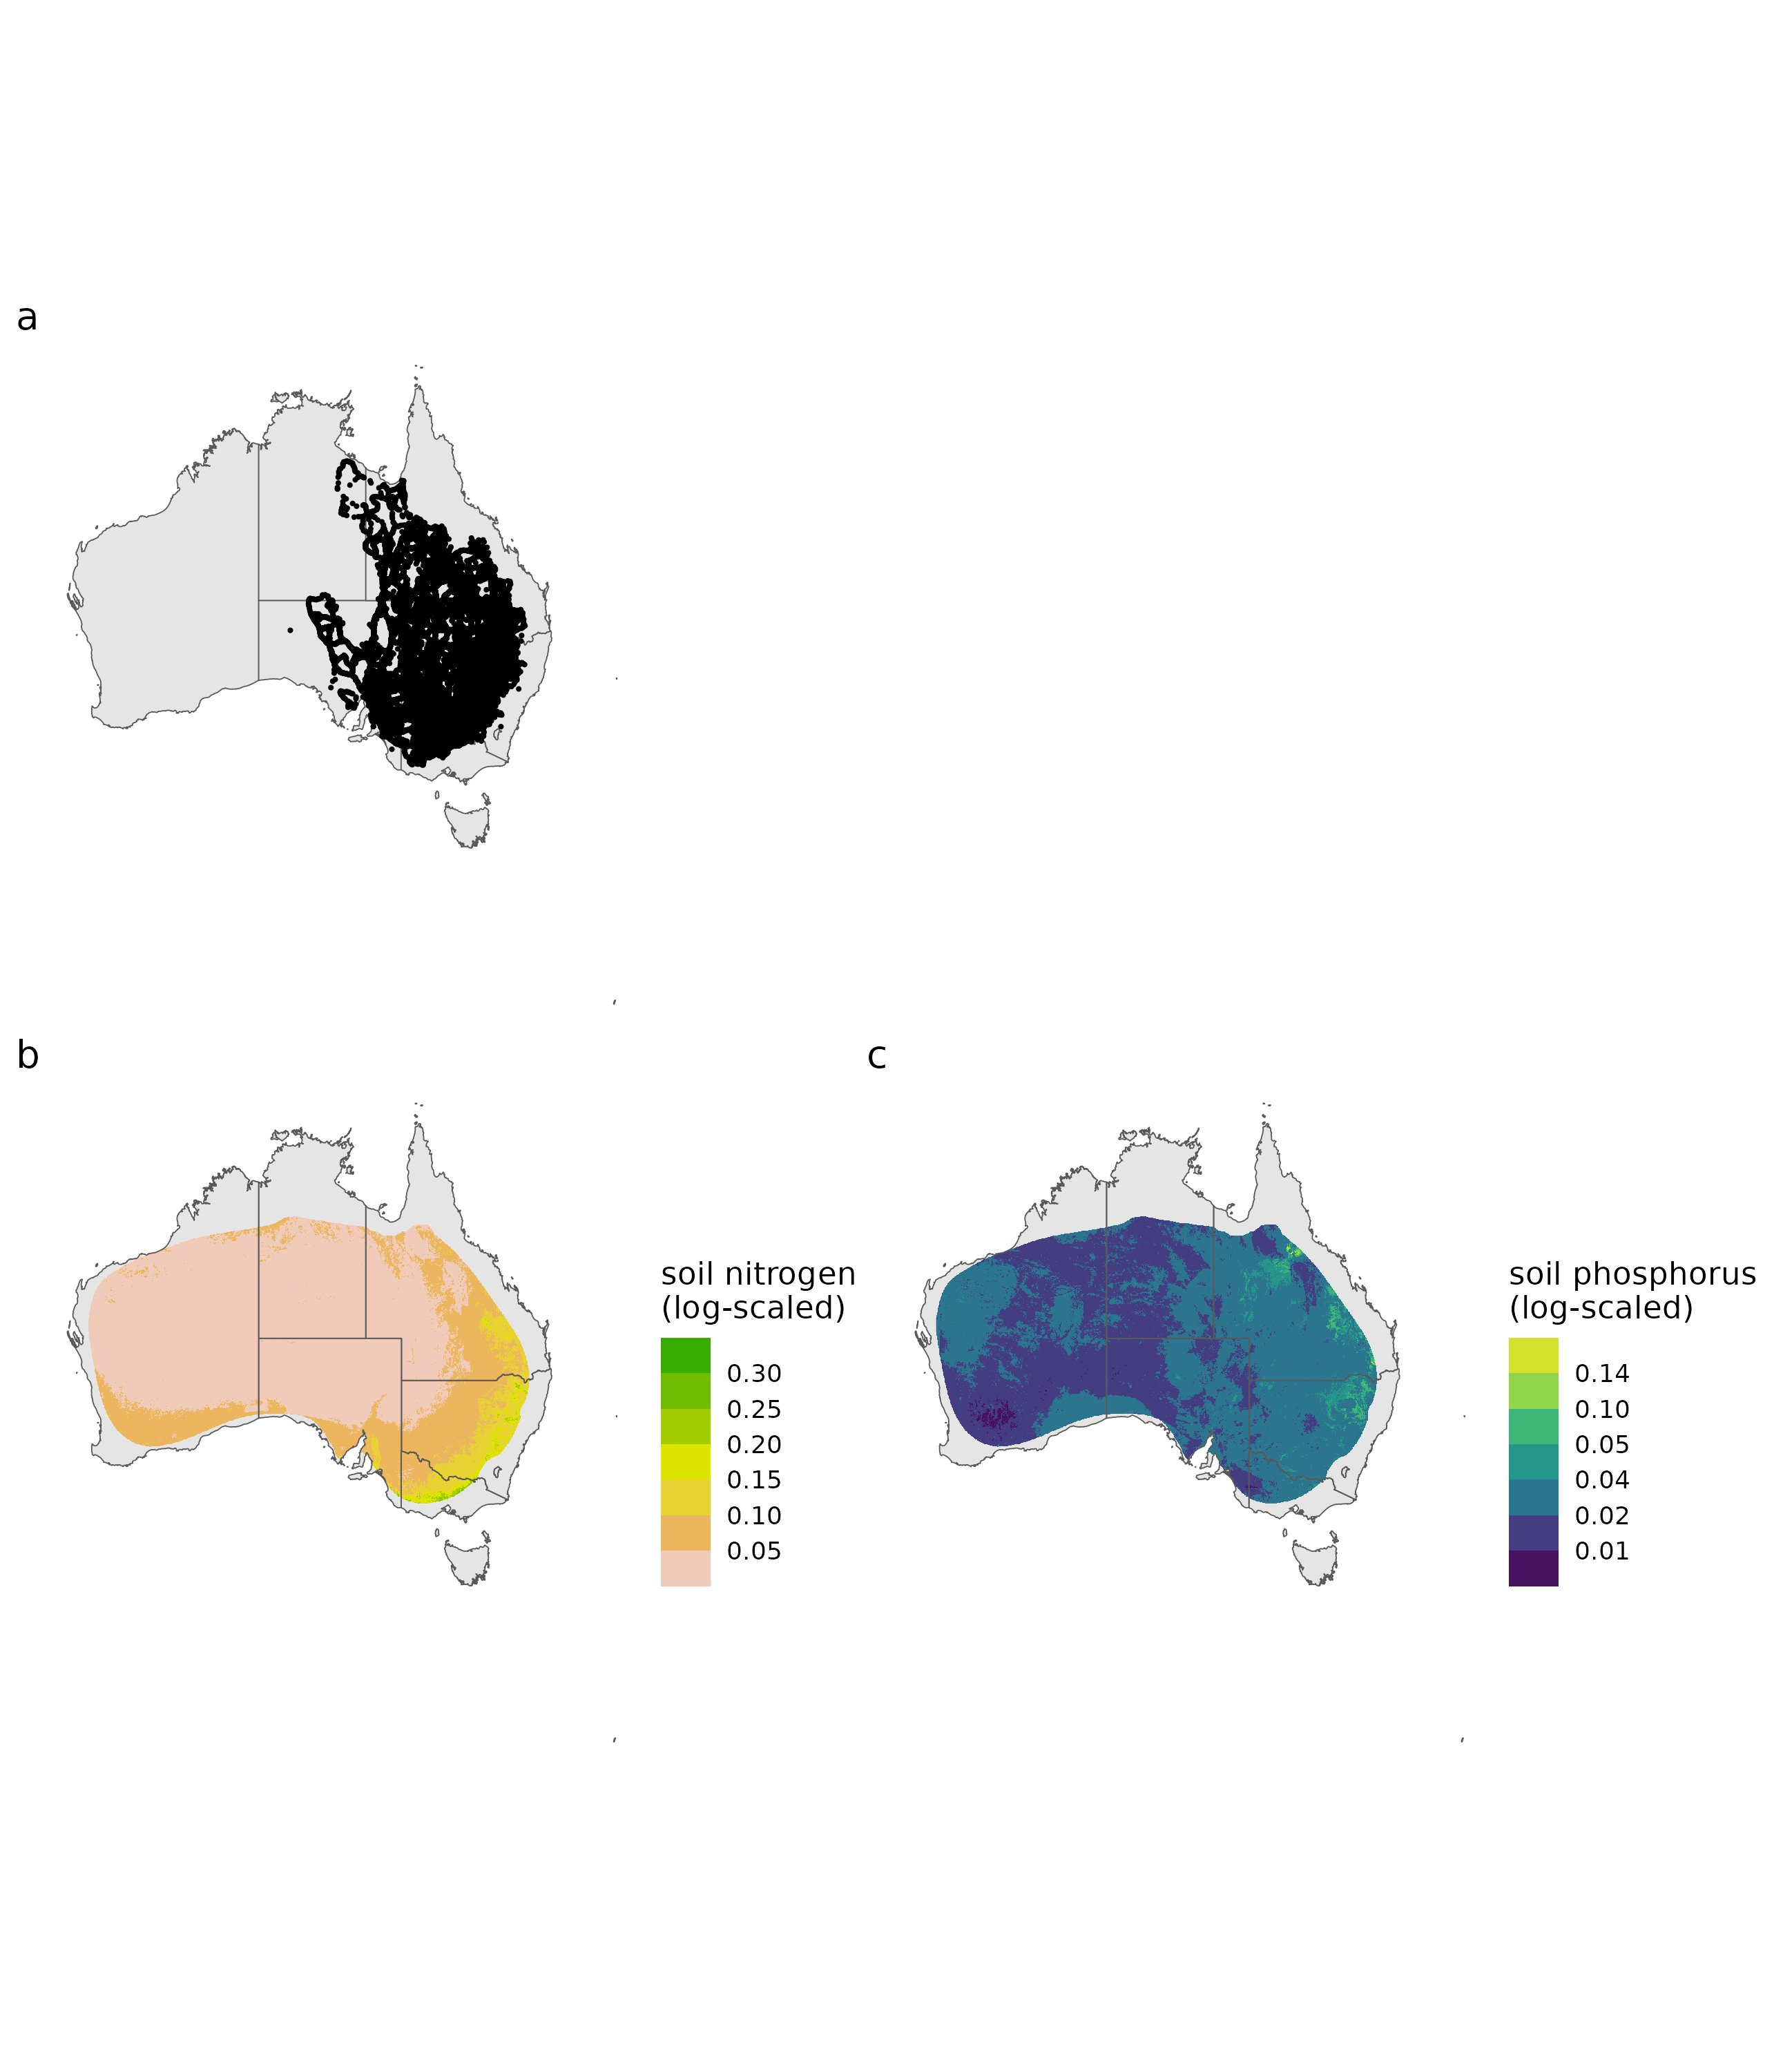
\includegraphics[keepaspectratio]{output/publication_figures/spatial_modeling_locust_env_map.png}}

}

\caption{\label{fig-spatial-modeling-env-map}Locust survey data map and
soil nutrients throughout the \emph{C. terminifera} distribution. A:
APLC survey dataset, B: mean proportion of nitrogen at 0-15 cm deep, C:
mean proportion phosphorous at 0-15cm deep.}

\end{fig}%

\subsection{Statistics}\label{statistics}

All statistics were conducted with either a generalized additive (mixed)
model or generlized linear (mixed) model approach when appropriate.This
allowed us to test for non-linear and linear trends in the dataset and
specify the hierarchical nature of the data. All statistics were
conducted in R and python. All scripts and packages used can be seen
within the project code repository:
\href{https://github.com/ddlawton/herbivore_nutrient_interactions}{github
repo}.

\subsubsection{Intake Targets (Question 1 and
2)}\label{intake-targets-question-1-and-2}

To determine intake targets, we constructed generalized additive model
(GAM) (family: Multivariate Normal Distribution, Link: Identity) with
the following variables when possible: diet pairing (factor), locust sex
(factor), time period interval (integer), locust initial weight
(numeric) following roughly the procedure found in
\citet{lawton_mismatched_2021}. We selected the inclusion of locust
weight as either a non-linear or linear effect via Akaike information
criterion (AIC), AIC adjusted for small sample size (AICc), and Bayesian
information criterion (BIC). If weight was not an important variable, it
was removed entirely from the model.

\subsubsection{Field population (Question
1)}\label{field-population-question-1}

We calculated intake targets as discussed above. To see the impact of
confined diet treatments on both specific growth rate and development
time, we constructed two linear models (family: gaussian, link:
identity) with the following variables: treatment (factor), locust sex
(factor), population (factor), and locust initial weight (numeric).

\subsubsection{Field Cage Experiments (Question
2)}\label{field-cage-experiments-question-2-1}

We assessed plant nutrients with a generalized additive mixed model
(GAMM) (family: Multivariate Normal Distribution, link: identity) and
included the following variables: plant carbohydrate (numeric,
dependent), plant protein (numeric, dependent), treatment (factor,
independent), cage (factor, random effect), plot (factor, random
effect), and plant species (random effect). Redressing intake targets
were conducted as discussed above (section 2.5.1). To see the difference
between physiological performance and fertilizer treatments, we
constructed GAMMs (family: Scaled T distribution, link: identity) for
final locust mass. The independent variables in all models were
treatment (factor), sex (factor), a two-dimensional smoother of
available protein and carbohydrate, and cage number as a random effect.
For both final adult proportion and survival proportion, we constructed
a GAM (Family: gaussian, Link: identity) and included the following
variables: treatment (factor) and a two-dimensional smoother of
available protein and carbohydrate.

\subsubsection{Historical outbreaks and soil nutrient grid modeling
(Question
3)}\label{historical-outbreaks-and-soil-nutrient-grid-modeling-question-3}

To relate nymph survey grids to soil nitrogen and phosphorus, we
constructed two GAMMs (family: tweedie, link: log) predicting the number
of outbreaks (APLC Survey Category 4) and nil observations (category 0).
Since soil nitrogen and mean annual precipitation are highly correlated
with both variables decreasing going into the arid interior of
Australia, we are unable to add precipitation directly to the model as
it would bias the results. Instead, we built a comparison model with
mean annual precipitation between 2000 and 2017 switched for soil
nitrogen. To do this, we calculated the average precipitation between
2000 and 2017 for all survey grids using the European Centre for
Medium-Range Weather Forecasts' ERA5 reanalysis dataset
\citep{munoz-sabater_era5-land_2021}. This allowed us to visually
compare the effect differences of soil nitrogen and mean annual
precipitation on locust outbreaks. In other words, if soil nitrogen and
mean annual precipitation were so tightly correlated that the effects
are indistinguishable, the modeled results should look very similar. The
soil models had the following independent variables: soil nitrogen,
phosphorus, latitude / longitude, bioregion, and the number of
observations within each grid. For the precipitation model, all
variables were the same except mean annual precipitation replaced soil
nitrogen and phosphorus. The inclusion of bioregions as a random effect
allowed us to account for variation due to vegetation community and soil
characteristics \citep{lawton_seeing_2022}. The inclusion of latitude
and longitude allowed us to account for spatial autocorrelation
\citep{clayton_spatial_1993}. Lastly, the inclusion of the total number
of observations allowed us to account for sampling intensity biases.

\section{RESULTS}\label{results}

\subsection{Field population (Question
1)}\label{field-population-question-1-1}

\subsubsection{Choice experiment (nutritional
target)}\label{choice-experiment-nutritional-target}

\emph{Chortoicetes terminifera} individuals from the two outbreaking
populations regulated to a specific ratio of 1 protein : 2 carbohydrate
(Figure~\ref{fig-field-pop-it-results}
A,Table~\ref{tbl-field-population-it-model}). Model selection can be
seen in
Supplementary Table~\ref{supptbl-field-population-choice-experiment-model-selection-criteria}.
Consumption in the two diet pairings did not differ, indicating that
instead of consuming between the diets randomly (which would be expected
if nutrients had no impact on diet consumption) locusts were actively
balancing their protein and carbohydrate consumption
(Supplementary Figure~\ref{suppfig-field-pop-nutrients} A,
Table~\ref{tbl-field-population-it-model}). While the protein :
carbohydrate ratio did not change, females consumed more food than
males, likely due to being bigger overall
(Supplementary Figure~\ref{suppfig-field-pop-nutrients} B,
Table~\ref{tbl-field-population-it-model}).

\begingroup
\fontsize{12.0pt}{14.4pt}\selectfont

\begin{longtable}{llrrr}

\toprule
macronutrient & variable & estimate & SE & p-value \\ 
\midrule\addlinespace[2.5pt]
carbohydrate & Intercept & 0.026 & 0.002 & 0.000 \\ 
 & Mendooran & -0.001 & 0.002 & 0.483 \\ 
 & diet pair B & 0.001 & 0.002 & 0.573 \\ 
 & male & -0.011 & 0.002 & 0.000 \\ 
protein & Intercept & 0.014 & 0.001 & 0.000 \\ 
 & Mendooran & -0.002 & 0.002 & 0.122 \\ 
 & diet pair B & 0.002 & 0.002 & 0.293 \\ 
 & male & -0.006 & 0.002 & 0.000 \\ 
\bottomrule

\caption{\label{tbl-field-population-it-model}Generalized additive model
results for macronutrient consumption (carbohydrate and protein) of two
outbreaking populations of \emph{C. terminifera} in Mendooran and
Guntawang. Models were selected via AIC, AICc and BIC which can be seen
in
Supplementary Table~\ref{supptbl-field-population-choice-experiment-model-selection-criteria}.
Diet pair A and B had the following protein to carbohydrate ratios:
7p:35c \& 28p:14c and 7p:35c \& 35p:7c respectively. Family:
multivariate gaussian distribution, link: identity, SE: standard error.}

\tabularnewline

\end{longtable}

\endgroup

\subsubsection{No choice experiment (performance
curves)}\label{no-choice-experiment-performance-curves}

\emph{Chortoicetes terminifera} had higher specific mass growth rates
and faster development times on the 1 protein : 2 carbohydrate (14
protein : 28 carbohydrate) diet as compared to the other diets
(Figure~\ref{fig-field-pop-it-results} B \& C,
Table~\ref{tbl-field-population-no-choice-model},
Supplementary Table~\ref{supptbl-field-population-no-choice-experiment-phys-post-hoc}).
Development time and specific growth rate did not differ between male
and female locusts
(Supplementary Figure~\ref{suppfig-field-pop-nutrients} C \& D,
Table~\ref{tbl-field-population-no-choice-model}).

\begin{fig}

\centering{

\pandocbounded{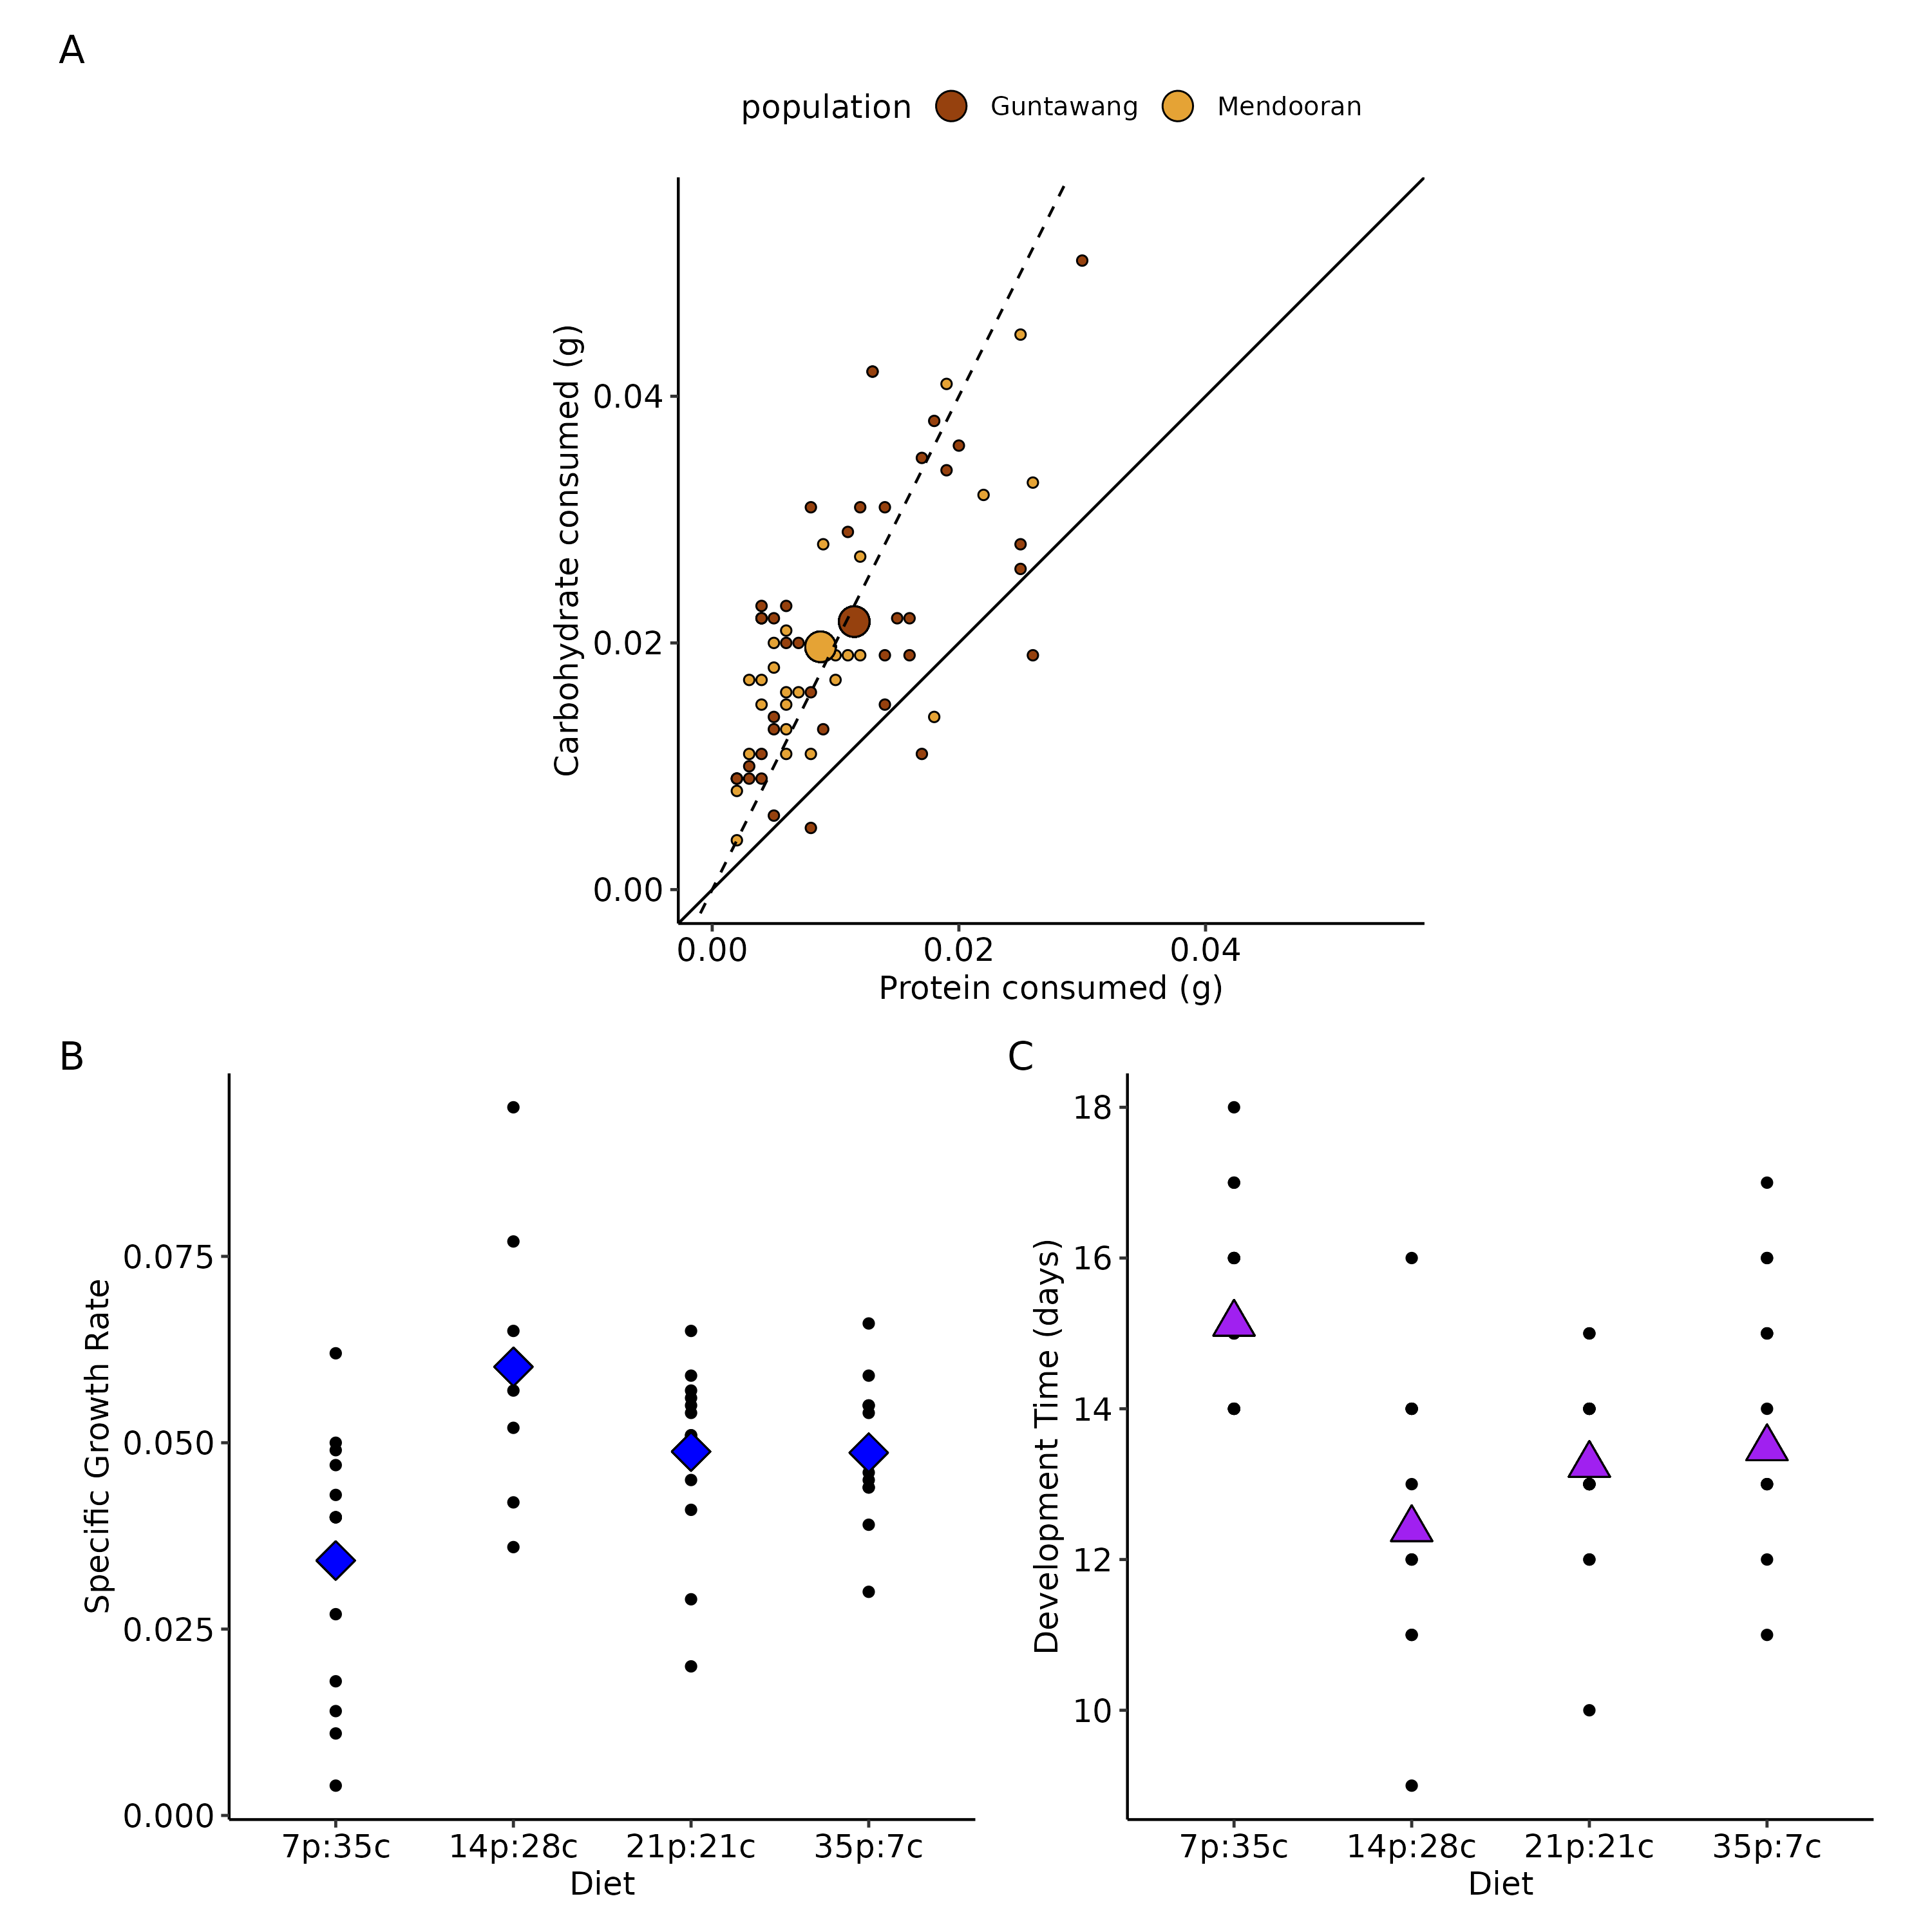
\includegraphics[keepaspectratio]{output/publication_figures/field_population_intake_target_figure.png}}

}

\caption{\label{fig-field-pop-it-results}The nutritional preference (A)
and physiological performance (B \& C) of \emph{C. terminifera}
individuals that were collected from two marching bands of 5th instars.
Raw data is shown as black dots with modeled estimated margial means as
large diamonds or triangles.}

\end{fig}%

\begingroup
\fontsize{12.0pt}{14.4pt}\selectfont

\begin{longtable}{lrrrrrr}

\toprule
 & \multicolumn{3}{c}{Specific Growth Rate} & \multicolumn{3}{c}{Development Time} \\ 
\cmidrule(lr){2-4} \cmidrule(lr){5-7}
variable & estimate & SE & p-value & estimate & SE & p-value \\ 
\midrule\addlinespace[2.5pt]
Intercept & 0.061 & 0.004 & 0.000 & 15.780 & 1.555 & 0.000 \\ 
21p:21c & -0.011 & 0.005 & 0.040 & 0.917 & 0.624 & 0.149 \\ 
35p:7c & -0.010 & 0.006 & 0.091 & 1.709 & 0.665 & 0.013 \\ 
7p:35c & -0.026 & 0.005 & 0.000 & 2.716 & 0.603 & 0.000 \\ 
male & -0.003 & 0.004 & 0.398 & -1.615 & 0.829 & 0.057 \\ 
initial weight (g) &  &  &  & -21.048 & 10.407 & 0.049 \\ 
\bottomrule

\caption{\label{tbl-field-population-no-choice-model}\emph{Chortoicetes
terminifera} physiological performance (specific growth rate and
development time) when constrained to specific diets with varying
protein and carbohydrate content. SE: standard error. Posthoc
comparisons for both physiological performance metrics can be seen in
Supplementary Table~\ref{supptbl-field-population-no-choice-experiment-phys-post-hoc}.}

\tabularnewline

\end{longtable}

\endgroup

\subsection{Field Cage (Question 2)}\label{field-cage-question-2}

For the first 11 days of the 14 day field cage experiment, plant protein
and carbohydrate contents remained consistently protein-biased for all
treatments (Figure~\ref{fig-field-cage-time-results} A-C,
Table~\ref{tbl-field-cage-plant-nutrients}), and only showed differences
in protein content by the last sample period on December 1, which was
after the end of the locust cage experiment. Accordingly, there was no
effect of fertilizer on locust survival and adult proportion
(Figure~\ref{fig-field-cage-time-results} D-F,
Table~\ref{tbl-field-cage-locust-mass}). Locusts that were retrieved
from field cages after nine days and were given a choice to regulate
protein and carbohydrate intake showed a pattern consistent with
rebalancing a shortage of carbohydrates
(Figure~\ref{fig-field-cage-it-rebalancing},
Table~\ref{tbl-field-cage-rebalancing},
Supplementary Figure~\ref{suppfig-field-cage-rebalancing-facet}).
Irrespective of fertilizer treatment group, locusts initially selected
very carbohydrate biased diets, but gradually, after 9 days, their
trajectory returned close to the predicted intake target of 1p : 2c
(Figure~\ref{fig-field-cage-it-rebalancing},
Supplementary Figure~\ref{suppfig-field-cage-rebalancing-facet}).

\begin{fig}

\centering{

\pandocbounded{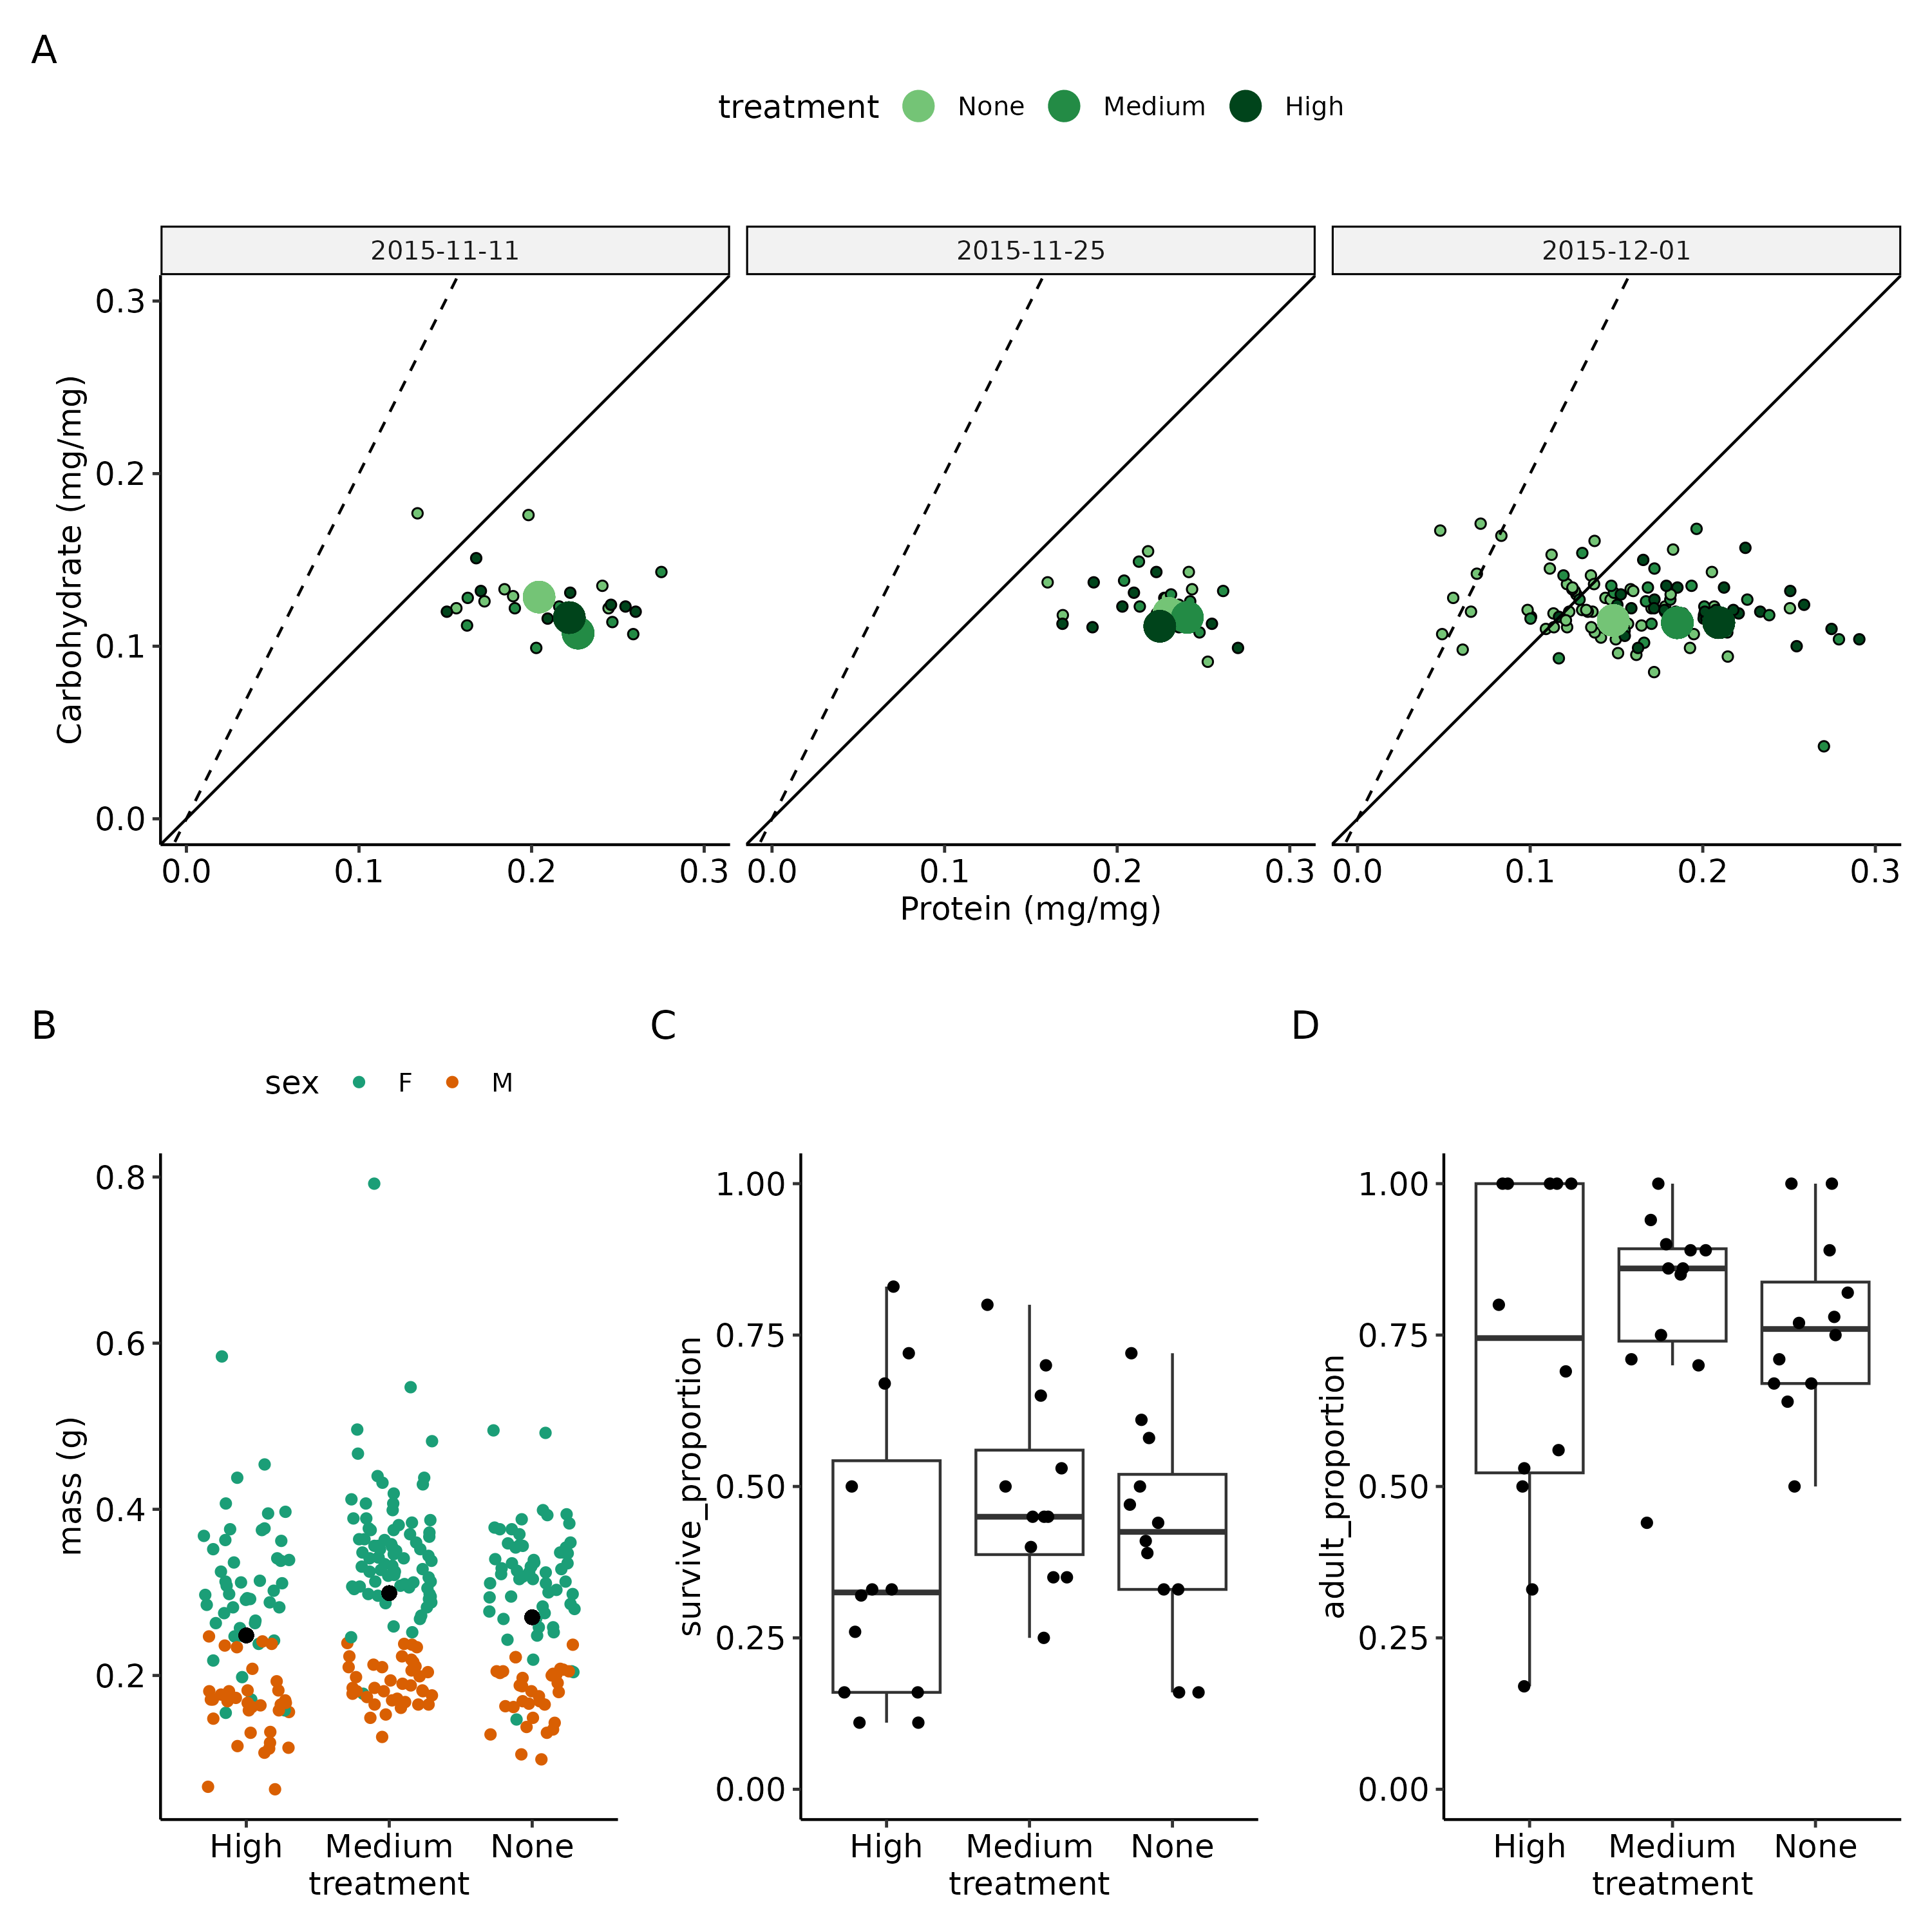
\includegraphics[keepaspectratio]{output/publication_figures/field_cage_plant_locust_figure.png}}

}

\caption{\label{fig-field-cage-time-results}Nitrogen addition field cage
experiments with plant nutrient change through time (A) and grasshopper
performance metrics (B-C) are shown. Dashed line represents a 1p : 2c
ratio, the solid line represents a 1p : 1c ratio. Black dots in B
represent overall means whereas boxplots represent the lower, median,
and upper quartlies.}

\end{fig}%

\begin{fig}

\centering{

\pandocbounded{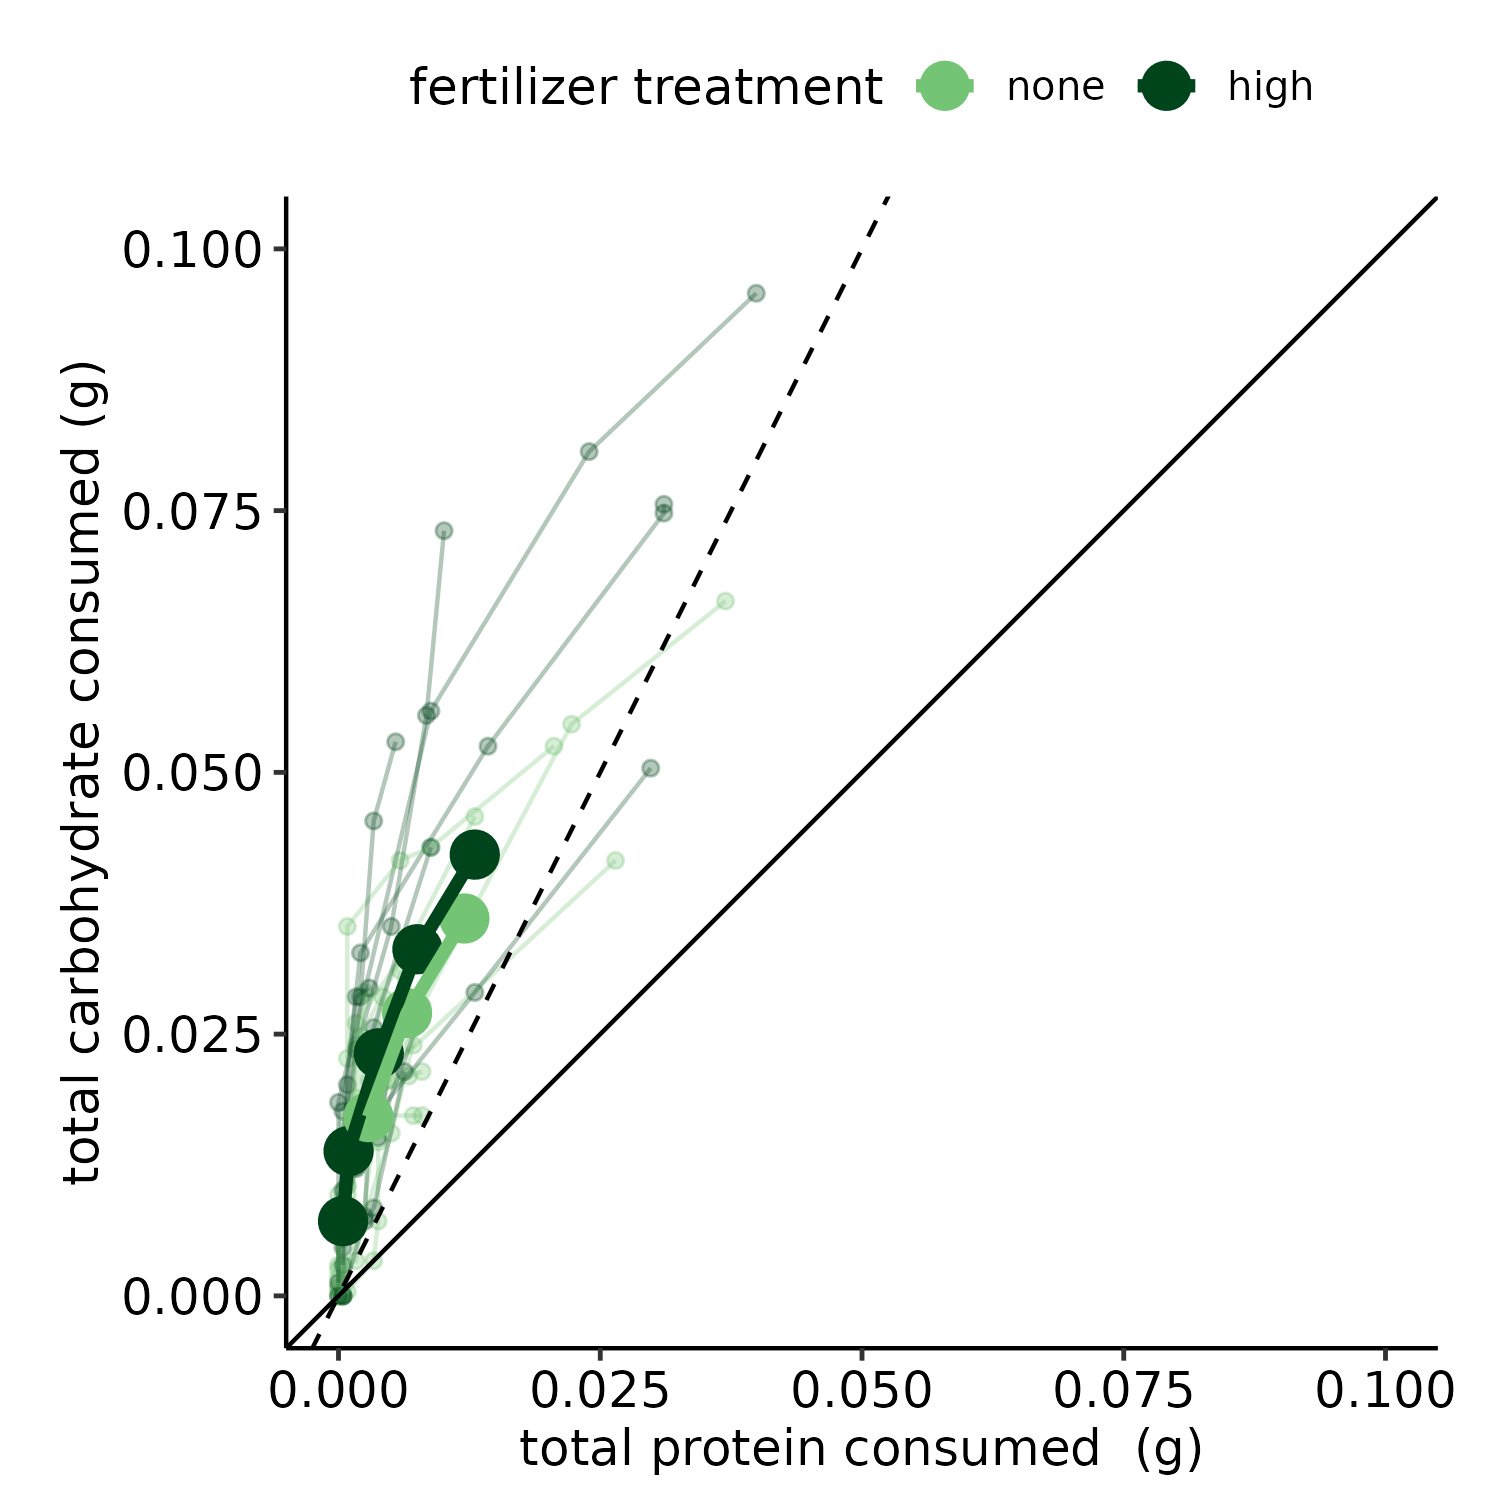
\includegraphics[keepaspectratio]{output/publication_figures/field_cage_locust_intake_target_rebalancing.png}}

}

\caption{\label{fig-field-cage-it-rebalancing}Nutrient imbalance
redressing with artificial diet mixing of \emph{C. terminifera}
individuals taken from fertilized treatment cages. Colors represent
fertilizer treatment. Smaller lines represent raw individual locust
intake targets; large lines and points represent estimated marginal
means. Points along each line represent sampling times on days 1, 2, 4,
6, and 9. Individual time step targets can be seen in
Supplementary Figure~\ref{suppfig-field-cage-rebalancing-facet}.}

\end{fig}%

\begingroup
\fontsize{12.0pt}{14.4pt}\selectfont

\begin{longtable}{llrrrr}

\toprule
macronutrient & variable & estimate & SE & statistic & p-value \\ 
\midrule\addlinespace[2.5pt]
carbohydrate & Intercept & 0.127 & 0.007 &  & 0.000 \\ 
 & Medium & -0.020 & 0.007 &  & 0.005 \\ 
 & High & -0.011 & 0.007 &  & 0.121 \\ 
 & 2015-11-25 & -0.009 & 0.007 &  & 0.181 \\ 
 & 2015-12-01 & -0.012 & 0.006 &  & 0.033 \\ 
 & Medium:2015-11-25 & 0.019 & 0.010 &  & 0.063 \\ 
 & High:2015-11-25 & 0.004 & 0.010 &  & 0.656 \\ 
 & Medium:2015-12-01 & 0.019 & 0.008 &  & 0.017 \\ 
 & High:2015-12-01 & 0.010 & 0.008 &  & 0.222 \\ 
 & s(species) &  &  & 67.305 & 0.000 \\ 
 & s(plot) &  &  & 1.643 & 0.207 \\ 
 & s(cage) &  &  & 3.442 & 0.130 \\ 
protein & Intercept & 0.209 & 0.017 &  & 0.000 \\ 
 & Medium & -0.001 & 0.014 &  & 0.928 \\ 
 & High & -0.034 & 0.014 &  & 0.014 \\ 
 & 2015-11-25 & 0.026 & 0.010 &  & 0.014 \\ 
 & 2015-12-01 & -0.049 & 0.009 &  & 0.000 \\ 
 & Medium:2015-11-25 & -0.012 & 0.015 &  & 0.422 \\ 
 & High:2015-11-25 & -0.023 & 0.015 &  & 0.123 \\ 
 & Medium:2015-12-01 & 0.008 & 0.013 &  & 0.516 \\ 
 & High:2015-12-01 & 0.056 & 0.013 &  & 0.000 \\ 
 & s(species) &  &  & 307.929 & 0.000 \\ 
 & s(plot) &  &  & 214.489 & 0.000 \\ 
 & s(cage) &  &  & 89.944 & 0.000 \\ 
\bottomrule

\caption{\label{tbl-field-cage-plant-nutrients}Generalized additive
model results for plant macronutrient (carbohydrate and protein)
differences between fertilization treatment. Family: multivariate
gaussian distribution, link: identity, SE: standard error, s() denotes a
smoothing parameter.}

\tabularnewline

\end{longtable}

\endgroup

\begingroup
\fontsize{12.0pt}{14.4pt}\selectfont

\begin{longtable}{lrrrr}

\toprule
variable & estimate & SE & statistic & p-value \\ 
\midrule\addlinespace[2.5pt]
Intercept & 0.326 & 0.007 &  & 0.000 \\ 
male & -0.148 & 0.006 &  & 0.000 \\ 
medium & 0.015 & 0.010 &  & 0.117 \\ 
high & -0.011 & 0.010 &  & 0.273 \\ 
s(carb mg/mg, protein mg/mg) &  &  & 0.002 & 0.416 \\ 
s(cage number) &  &  & 42.160 & 0.000 \\ 
\bottomrule

\caption{\label{tbl-field-cage-locust-mass}Generalized additive model
results for differences between final locust mass after the nitrogen
fertilization experiment finished. Family: scaled T, link: identity, SE:
standard error, and s() denotes a smoothing parameter.}

\tabularnewline

\end{longtable}

\endgroup

\begingroup
\fontsize{12.0pt}{14.4pt}\selectfont

\begin{longtable}{llrrrr}

\toprule
macronutrient & variable & estimate & SE & statistic & p-value \\ 
\midrule\addlinespace[2.5pt]
carbohydrate & Intercept & 0.013 & 0.004 &  & 0.001 \\ 
 & male & -0.011 & 0.004 &  & 0.009 \\ 
 & day 2 & 0.007 & 0.003 &  & 0.008 \\ 
 & day 3-4 & 0.016 & 0.003 &  & 0.000 \\ 
 & day 5-6 & 0.026 & 0.003 &  & 0.000 \\ 
 & day 7-9 & 0.035 & 0.003 &  & 0.000 \\ 
 & none & -0.006 & 0.004 &  & 0.136 \\ 
 & s(id) &  &  & 484.706 & 0.000 \\ 
protein & Intercept & 0.002 & 0.001 &  & 0.119 \\ 
 & male & -0.004 & 0.001 &  & 0.009 \\ 
 & day 2 & 0.001 & 0.001 &  & 0.724 \\ 
 & day 3-4 & 0.003 & 0.001 &  & 0.023 \\ 
 & day 5-6 & 0.007 & 0.001 &  & 0.000 \\ 
 & day 7-9 & 0.013 & 0.001 &  & 0.000 \\ 
 & none & -0.001 & 0.001 &  & 0.475 \\ 
 & s(id) &  &  & 110.728 & 0.381 \\ 
\bottomrule

\caption{\label{tbl-field-cage-rebalancing}Generalized additive model
results for nutrient imbalance dressing of field cage \emph{C.
terminifera} in the control and high fertilization treatments. Model
also included interactive terms; however, none were significant and left
out. SE: standard error and s() denotes a smoothing parameter.}

\tabularnewline

\end{longtable}

\endgroup

\subsection{Locust outbreaks (Question
3)}\label{locust-outbreaks-question-3}

\emph{Chortoicetes terminifera} outbreaks were negatively associated
with soil nitrogen, which supports the hypothesis that nitrogen (in
excess) acts as a limiting factor for population upsurges
(Table~\ref{tbl-spatial-modeling-outbreak-model-results},
Figure~\ref{fig-spatial-model-nto-pto} A). \emph{C. terminifera}s had a
nonlinear relationship with soil phosphorus with outbreaks occurring
more often in areas with approximately 4\% soil phosphorus and were
strongly negatively associated with increasing phosphorus afterwards
(Figure~\ref{fig-spatial-model-nto-pto} B). For both nutrients, the
absence models had a very weak relationship with soil nutrient in
comparison to the outbreak models, demonstrating little model bias due
to APLC survey protocol. There were significant nonlinear relationships
between coordinates and the total number of observations in all models
(Supplementary Figure~\ref{suppfig-spatial-modeling-outbreak-all-vars};
Supplementary Figure~\ref{suppfig-spatial-modeling-nil-all-vars}). The
relationship between locust outbreaks and mean annual precipitation was
very different from the relationship with soil nitrogen (
Figure~\ref{fig-spatial-model-nto-pto},
Supplementary Figure~\ref{suppfig-spatial-modeling-map-outbreak-corr}).
Soil nitrogen and phosphorus show weak positive correlations with woody
vegetation cover, while mean annual precipitation exhibits high
variation in its relationship with soil nitrogen and weak correlation
with soil phosphorus
(Supplementary Figure~\ref{suppfig-spatial-modeling-env-corr}). Thus,
the relationship between soil nitrogen and locust outbreaks cannot be
fully explained by differences in woody vegetation.

\begin{fig}

\centering{

\pandocbounded{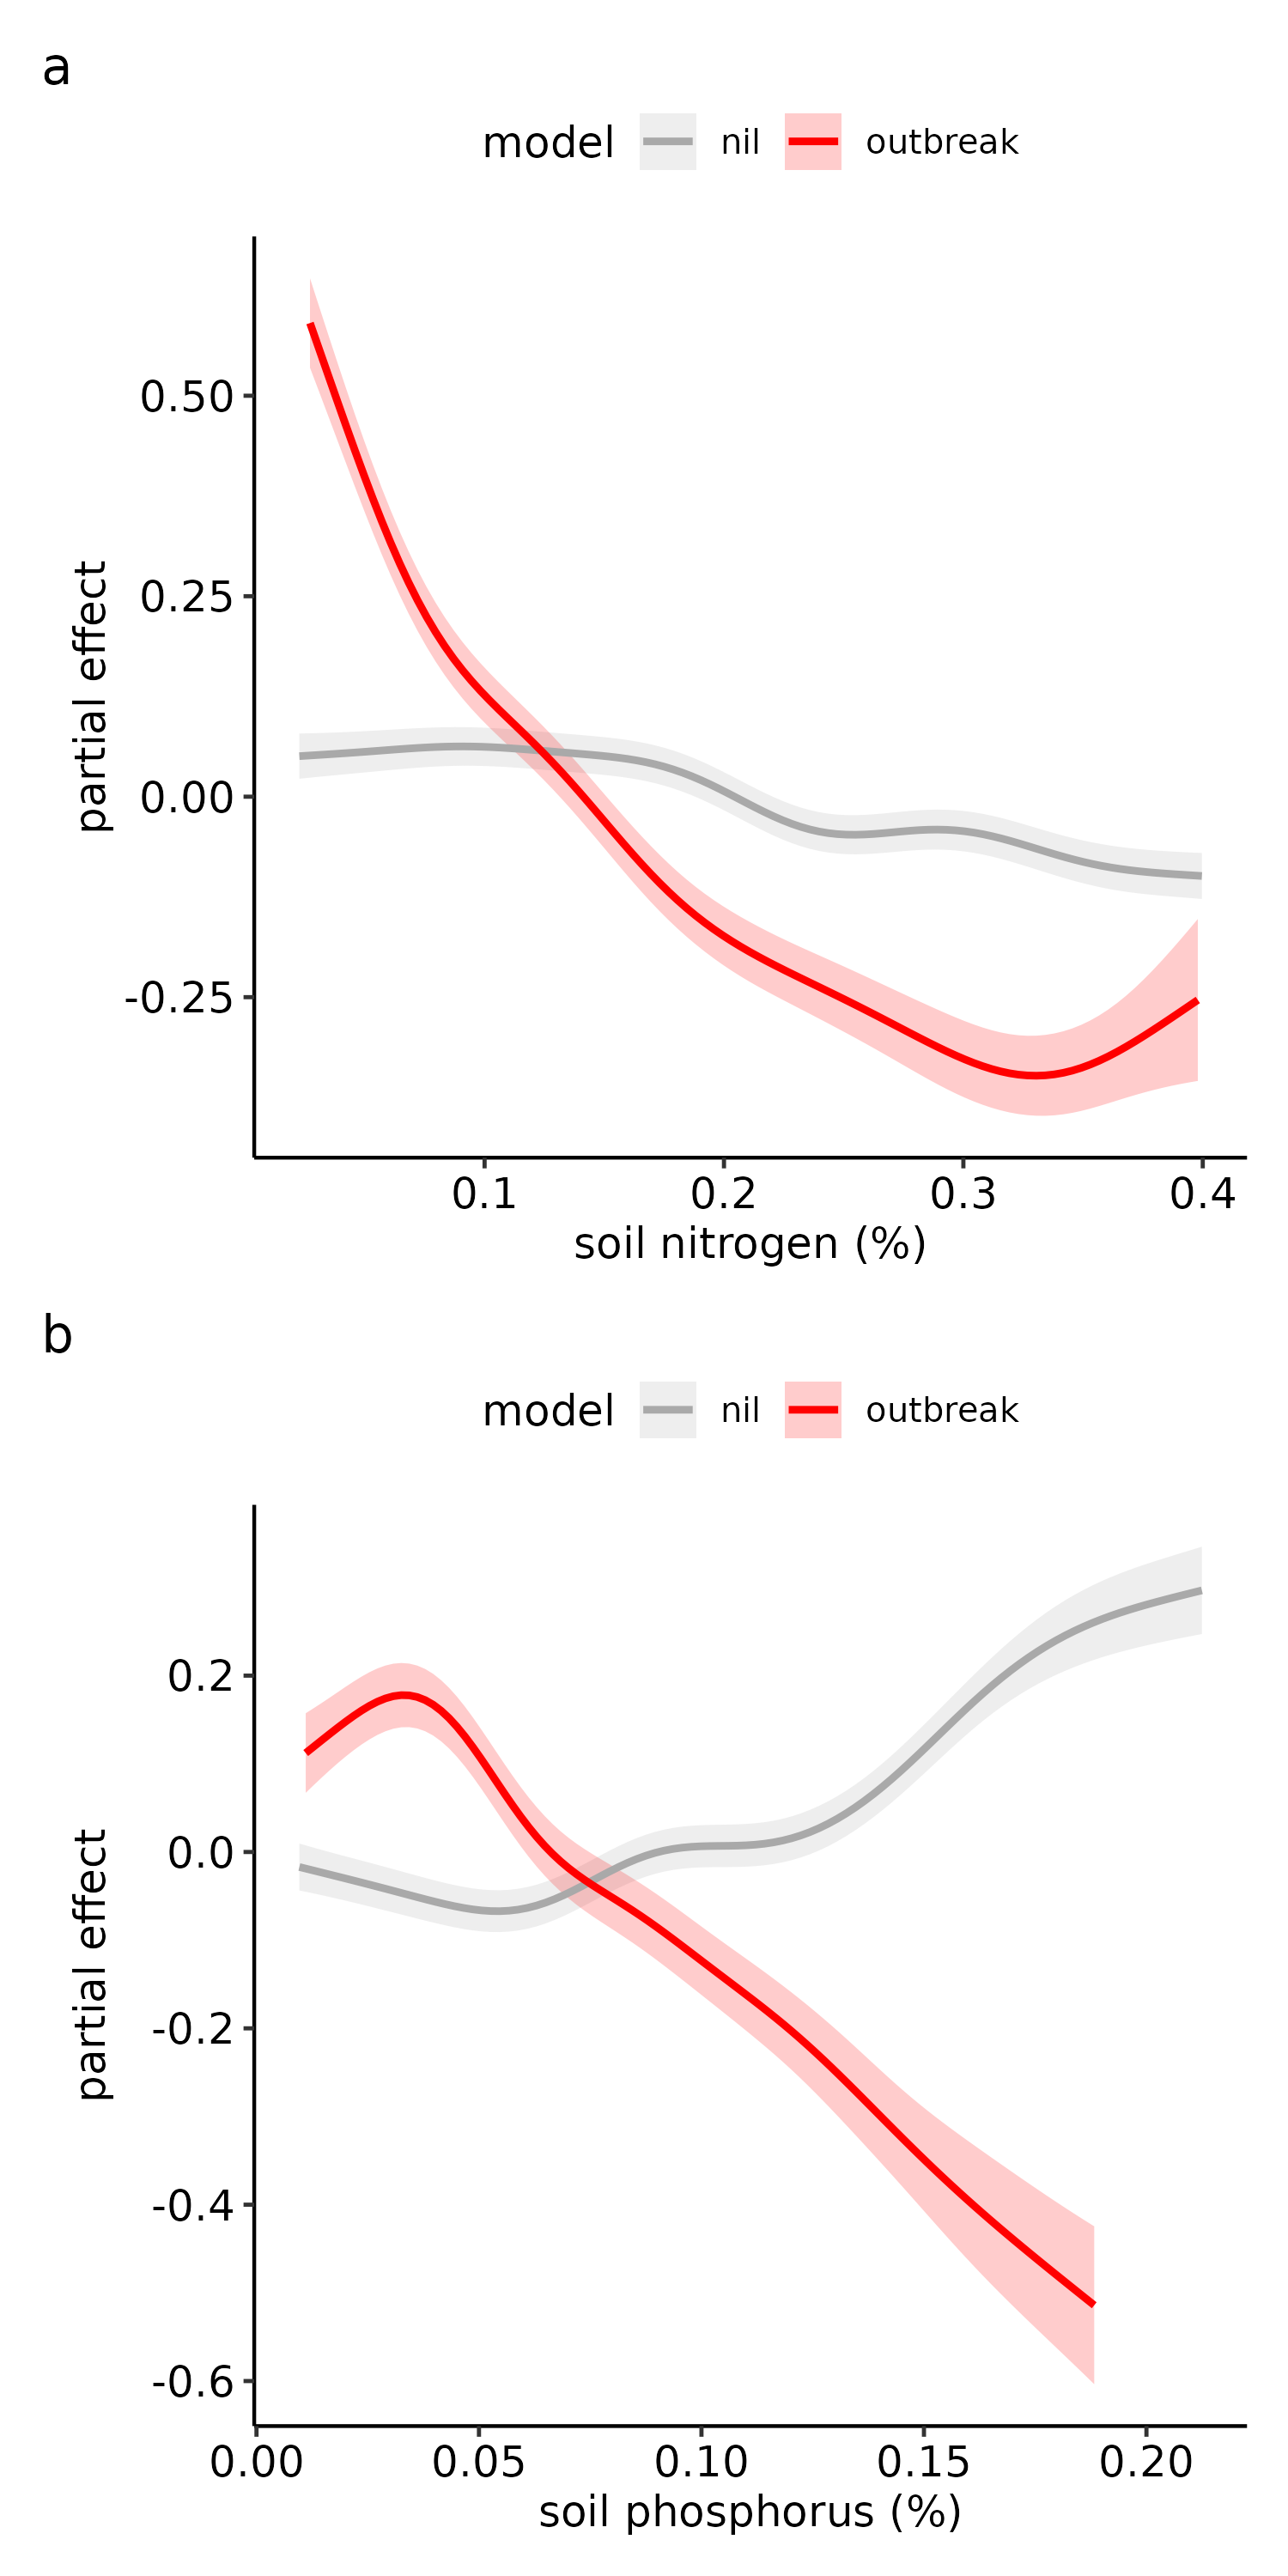
\includegraphics[keepaspectratio]{output/publication_figures/spatial_modeling_locust_outbreak_with_soil_NTO_PTO.png}}

}

\caption{\label{fig-spatial-model-nto-pto}Relationship between outbreaks
and nil observations for both soil nitrogen (A) and phosphorus (B).
Partial effect is the modeled predictions after accounting for bioregion
and spatial autocorrelation.}

\end{fig}%

\begingroup
\fontsize{12.0pt}{14.4pt}\selectfont

\begin{longtable}{lrrrrrr}

\toprule
 & \multicolumn{3}{c}{outbreak model} & \multicolumn{3}{c}{nil model} \\ 
\cmidrule(lr){2-4} \cmidrule(lr){5-7}
variable & EDF & statistic & p-value & EDF & statistic & p-value \\ 
\midrule\addlinespace[2.5pt]
s(nitrogen) & 6.273 & 25.620 & 0.000 & 6.426 & 35.340 & 0.000 \\ 
s(phosphorus) & 5.372 & 15.521 & 0.000 & 6.407 & 28.867 & 0.000 \\ 
s(number of observations) & 22.547 & 630.896 & 0.000 & 22.408 & 3,199.357 & 0.000 \\ 
te(longitude,latitude) & 56.140 & 1.148 & 0.012 & 131.476 & 3.302 & 0.000 \\ 
s(ecoregion) & 6.498 & 4.802 & 0.000 & 2.726 & 0.361 & 0.035 \\ 
\bottomrule

\caption{\label{tbl-spatial-modeling-outbreak-model-results}Historical
locust presence data modeling with soil nitrogen for outbreak, low
presence, and no observation records with r-square and deviance explain
reported. Family: tweedie, link: log, edf = estimated degrees freedom.}

\tabularnewline

\end{longtable}

\endgroup

\section{DISCUSSION}\label{discussion}

We show that herbivore diet preferences remain consistent between
spatial levels, from individual foraging behavior and physiology to
large scale population dynamics, with locust populations negatively
related to environmental nitrogen. Thus by going across scales, this
study shows a consistent pattern of excess nitrogen limiting a pest
herbivore and introduces a more nuanced view of phosphorus limitation on
herbivore populations. Instead of the broad generalization that animals
are always negatively or positively associated with certain nutrients,
specific life history traits, such as energetically-costly migration, as
well as organism-environment interactions should be considered. While
this study advances our understanding of nutrient limitation across
scales, future work should explicitly assess phosphorus nutrient
imbalances at finer scales to clarify their influence on broader
patterns of herbivore population dynamics. Investigating multi-scale
nutrient interactions, including a wider array of nutrients such as
potassium and sodium, could also provide a more comprehensive framework
for modeling herbivore responses to environmental heterogeneity. For
forecasting pest populations dynamics, describing the nutritional
quality of landscapes can inform seasonal scouting surveys. We hope that
this study spurs future interest in multi-scale experiments and modeling
of nutrient availability with animal population dynamics.

\subsection{Field populations}\label{field-populations}

Field populations of final instar \emph{C. terminifera} behaviorally
regulated to a 1 protein (p) : 2 carbohydrate (c) nutrient ratio, which
supported the fastest nymphal growth and the lowest development time to
adulthood (Figure~\ref{fig-field-pop-it-results} B \& C), consistent
with previous studies
\citep{clissold_regulation_2014, lawton_mismatched_2021}. Locusts are
highly mobile (\emph{C. terminifera} can fly up to 500 km in a single
night, \citep{deveson_not_2005}) and the demand for energy via
carbohydrates and lipids likely increases relative to protein demand
during the later life stages of these animals.

Plant nutrient content in the nitrogen fertilization treatments was not
significantly different until the last sample period, which likely
explains the small effect on locust growth
(Figure~\ref{fig-field-cage-time-results} A-C). Over the experimental
period, protein content decreased in unfertilized treatments while both
plant protein and carbohydrate remained constant in the fertilized
treatments. If we prolonged the experiment, there might have been a
noticeable difference in locust survivorship, weight gain, and adult
proportion given the shift in nutrients among treatments
(Figure~\ref{fig-field-cage-time-results} D-F).

Importantly, all field cage plants were protein biased (roughly 1p : 1c
to 2p : 1c ) as compared to the desired locust intake target of 1p : 2c.
When locusts were subsampled from the field cages mid-experiment and
given the opportunity to select carbohydrate or protein diets, they
selected extremely carbohydrate-biased diets for more than a week. This
behavior indicated that locusts in the small field cages were highly
carbohydrate-limited, driving them to overeat carbohydrates to redress
the imbalance. Interestingly, multiple studies have shown that the
Australian nutritional landscape is often too protein-biased relative to
what the \emph{C. terminifera} prefers
\citep{lawton_woody_2020, lawton_mismatched_2021}. Regardless,
populations are still persistent and outbreaks can occur at lower
frequencies in these areas
\citep{deveson_satellite_2013, key_general_1945}. How this species can
achieve the optimal balance of nutrients within an unfavorable
nutritional environment merits further investigation, but may include
post-ingestive regulation and/or large-range foraging. Migratory locusts
(\emph{Locusta migratoria}) can choose microclimates that favor higher
efficiency of carbohydrate or protein absorption depending on their host
plant and nutritional status \citep{clissold_insect_2013}. For this
study, we collected free-living locusts from the same region and a
similar environment as where we built the field cages, yet those
confined to field cages selected a 10x decrease in p:c (1p : 20c vs 1p :
2c). This result suggests that free-living locusts are able to persist
in high protein regions by foraging over a larger range to seek out
pockets of carbohydrate-rich plants and that the limited foraging range
of the field cages precluded field-cage locusts from finding sufficient
carbohydrates. Similarly, these results suggest that, while \emph{C.
terminifera} can persist in low numbers in nitrogen rich regions, those
environments are unlikely to support extreme outbreaks due to a
limitation of carbohydrate-rich resources.

\subsection{Historical outbreak
modeling}\label{historical-outbreak-modeling}

This is the first time to our knowledge that terrestrial animal
population dynamics have been modeled with nutrients at the continental
level, allowing nutrient limitation to be tested at a scale not
previously investigated. Locust outbreaks are associated with less soil
nitrogen (Figure~\ref{fig-spatial-model-nto-pto} A), suggesting that
nitrogen acts as a limiting factor not due to its deficit
\citep{white_inadequate_1993} but its excess. Plants growing in high
nitrogen environments tend to have high p:c ratios, which force locusts
to either undereat carbohydrates (limiting their energy to support
growth and migration) or overeat protein (which can be toxic) to acquire
sufficient carbohydrates \citep{behmer_insect_2009, cease_how_2024}. On
the other end of the performance curve, \emph{C. terminifera} do have a
lower p:c range that limits performance, as shown using artificial diets
(Figure~\ref{fig-field-pop-it-results} B-C). We also show that outbreaks
are correlated with a low level of soil phosphorus, however, outbreaks
peak at approximately 4\%, suggesting that while locusts generally do
well in low phosphorus environments, phosphorus deficit can be limiting
for locusts in extremely phosphorus poor soils
(Figure~\ref{fig-spatial-model-nto-pto} B). Because Australian soils are
characteristically phosphorus poor \citep{donald_colin_phosphorus_1964},
Australian animals like this locust are adapted to phosphorus poor
environments and potentially having too much phosphorus is deleterious
\citep{morton_fresh_2011}. Locust populations may be more tightly
correlated with soil nitrogen than phosphorus because terrestrial
herbivores require 5-50 times more nitrogen than phosphorus
\citep{elser_nutritional_2000}, meaning they can more readily balance
phosphorus by eating a few foods rich or poor in phosphorus but cannot
as quickly regulate protein and carbohydrate energy because they make up
the bulk of their required nutrients. Indeed, laboratory studies have
revealed that short-term limitations in dietary phosphorus have no
apparent impact on grasshopper growth \citep{cease_dietary_2016},
suggesting that these mobile herbivores could seek out phosphorus-rich
diets intermittently to overcome potential phosphorus limitation in
field environments. However, in this study, we only tested this
relationship with phosphorus at the continental level; further field and
laboratory experiments are needed to explore this non-linear
relationship between locust outbreaks and soil phosphorus. While we only
looked at nitrogen and phosphorus, it is also important to note that
animals require a suite of nutrients. Other nutrients such as potassium
and sodium \citep{joern_not_2012} warrant further investigation.
Comparing locust outbreaks between continents would further show the
relationship between nutrient availability and animal population
dynamics. One excellent dataset for this would be SoilGrids
(https://www.isric.org/explore/soilgrids) which provides soil nitrogen
estimates globally at a 250-meter resolution.

Lastly, our results suggest that forecasting efforts for locusts should
consider the inclusion of a nutritional landscape quality metric like
soil nitrogen. Current forecasting models use climatic data
(e.g.~rainfall and soil moisture) or vegetation growth data
(e.g.~normalized difference vegetation index, NDVI) as the major
predictors of outbreaks \citep{cressman_role_2013}. While these climatic
variables are clearly important, adding metrics to quantify the
nutritional landscape can help increase forecasting model accuracy in
environments with highly variable climates.

\subsection{Locusts are more likely to be limited by high nitrogen
environments than other
grasshoppers}\label{locusts-are-more-likely-to-be-limited-by-high-nitrogen-environments-than-other-grasshoppers}

A five-decade review of grasshopper responses to plant nitrogen content
showed that grasshoppers not classified as locusts have a variation of
negative, neutral, and positive responses to increasing plant nitrogen
\citep{cease_how_2024}. Looking just at field surveys, there are more
reports of a negative correlation between plant nitrogen and non-locust
grasshopper abundance (17 reports) relative to neutral (6 reports) or
positive (9 reports). This pattern corroborates long-term studies
showing that dilution of plant nitrogen is correlated with declines of
North American grasshopper populations \citep{welti_nutrient_2020}. Of
the studies that report positive correlations between individual
grasshopper species abundance and plant nitrogen, most are from
graminivorous (grass-feeding) species (11 reports), with 7 reports from
mixed (grasses and forbs) or forb feeders \citep{cease_how_2024}. This
pattern supports the hypothesis that grass-feeders are more likely to be
nitrogen-limited because grasses tend to have lower p:c ratios than
forbs; although this trend was not significant and grass-feeders also
regularly showed negative responses to high plant nitrogen. In contrast,
there was a consistent negative effect of high plant nitrogen on locust
species, regardless of whether they were graminivorous or mixed feeders.
Because mass specific protein consumption is highly correlated with
growth rate in both lab and field populations, but carbohydrate
consumption is highly influenced by the environment
\citep{talal_body_2024}, it is most likely that locusts have similar
protein requirements as other non-locust grasshopper species, but have
much higher carbohydrate demands, potentially to support migration
\citep{raubenheimer_integrative_1997, talal_high_2021, talal_body_2024}.
Locusts are able to meet this increased demand for carbohydrate, while
keeping protein consumption constant, by eating larger amounts of low
p:c plants found in low nitrogen environments. In summary, these studies
suggest that nymphal outbreaks of all locust species may be negatively
correlated with soil nitrogen across continental scales, but that the
correlation between plant nitrogen and non-locust grasshoppers may not
be significant or consistent through space and time.

\subsection{Comparing the relationship between plant macronutrients and
herbivore abundance in other
taxa}\label{comparing-the-relationship-between-plant-macronutrients-and-herbivore-abundance-in-other-taxa}

The effect of plant protein and carbohydrate on herbivore populations is
predicted to depend on the herbivore's p:c intake target (IT) relative
to its nutritional landscape (Le Gall et al., 2020). If there are
sufficient plants on either side of the IT, herbivores can select from
between them to achieve their IT. This complementary feeding has been
recorded for field populations of blue sheep (\emph{Psuedois nayaur}) in
the Himalayan Mountains \citep{aryal_foods_2015}, Black Howler Monkeys
(\emph{Alouatta pigra}) in Yucatán \citep{bridgeman_feeding_2012}, and
other primates \citep{raubenheimer_nutritional_2013}. There would be a
predicted impact on populations if the nutritional landscape were to
become more constricted or not overlap with the IT. For example, lab
colonies of tobacco hornworms (\emph{Manduca sexta} larvae) have an IT
around 1:1 or sometimes slightly carbohydrate-biased
\citep{wilson_dietary_2019} and their host plants tend to be
carbohydrate-biased relative to their IT
\citep{wilson_nutritional_2019}. However, this does not seem to
translate to population level effects, potentially due to secondary
metabolites affecting growth more strongly than macronutrient balance
and/or larvae may be able to compensate by overeating carbohydrates to
acquire sufficient protein \citep{wilson_dietary_2019}. Overeating
carbohydrates is not as detrimental as overeating protein, at least in
the short term, and animals tend to be willing to overeat carbohydrates
to a greater extent than protein
\citep{cheng_geometry_2008, simpson_nature_2012}. Therefore, herbivores
facing a nutritional landscape with a p:c generally lower than their IT
(i.e., carbohydrate excess) may not be as negatively impacted as
herbivores facing one higher than their IT (i.e., protein excess).
However, there are several examples of higher localized densities of
herbivores in response to higher plant nitrogen and protein contents
with thrips \citep{brown_relationship_2002} and spruce budworm
(\emph{Choristoneura}) \citep{de_grandpre_defoliation-induced_2022}
being two examples. These examples suggest that low p:c diets limit
population growth of some herbivores, but more studies are needed to
determine if this relationship is only localized or if it scales up. It
may be that herbivore populations with lower numbers are not limited by
a nutritional landscape at a large scale because they can differentially
disperse locally among optimal patches, whereas herbivore populations
with extreme numbers (i.e., irruptions) may be more limited by
nutritionally unfavorable environments across scales.

Herbivore responses to nutrient variation often exhibit species-specific
patterns, even among closely related species within the same feeding
guild. For instance, generalist grasshoppers (\emph{Melanoplus} spp.)
coexist by occupying distinct nutritional niches, varying their
protein-to-carbohydrate intake ratios despite consuming overlapping host
plants \citep{behmer_coexisting_2008}. Similarly, \emph{Euchorthippus
cheui} and \emph{E. unicolor} display opposing preferences for
nitrogen-enriched versus nitrogen-depleted host plants, leading to
divergent population responses to fertilization and grazing pressure
\citep{zhu_phenology_2020, zhu_constrasting_2023}. These examples
highlight how phenological or physiological differences shape responses
to shared nutritional landscapes. Building on these findings, we
hypothesize that related locust species, including \emph{Chortoicetes
terminifera}, may also exhibit distinct nutrient preferences,
potentially driven by local adaptations to environmental conditions.
Investigating these differences could provide insights into how nutrient
availability influences herbivore population dynamics across ecological
scales.

There is evidence for phosphorus limitation in some species, but limited
research showing a detrimental effect of excess phosphorus
\citep{cease_dietary_2016}. In aquatic insects such as \emph{Daphnia}
species, there is a strong positive association with phosphorus
available and population dynamics \citet{andersen_stoichiometry_2004}.
However this trend is not seen in field cricket populations
(\emph{Gryllus veletis}) \citep{harrison_synthesis_2014} and other
terrestrial insects. \citet{loaiza2011} found no effect of phosphorus
fertilization (but a positive effect of N fertilization) on Kansas
tallgrass prairie grasshopper population distributions, whereas
\citet{joern_not_2012} found consistent positive correlations between
plant phosphorus and Nebraskan grassland grasshopper populations.

Making predictions about a population's nutritional demands can aid in
making predictions about the relationship between nutritional landscapes
and population dynamics. Across taxa, including fish, chickens, rats,
cats, caribou, pigs, and dairy cattle, mass specific protein consumption
is highly correlated with growth rate and decreases with age and body
size \citep{talal_body_2024}. In contrast, energy demand (carbohydrates
and lipids) does not show a clear relationship with growth rate and
instead is more affected by environment and activity
\citep{talal_body_2024}. Therefore, an animal's IT is predicted to be
affected by the contrasting effects of growth (increases dietary p:c)
and activity or stress (increases carbohydrate demand and therefore
decreases dietary p:c), although other physiological and environmental
factors affect p:c demand as well (see Table 1 in
\citet{cease_how_2024}). For example, monarch butterflies have been
gradually increasing their already-high daily energy expenditure during
migration due to warmer temperatures caused by climate change
\citep{parlin_cost_2023}. Young and fast growing herbivores with low
activity levels would be predicted to have a high p:c IT, whereas older
juveniles and adults (slower mass specific growth) with high activity
levels would be predicted to have a low p:c IT. Comparative studies with
herbivores grouped functionally, such as other highly migratory animals
(e.g.~across insects, birds, mammals, and fish), or by growth rate or
developmental stage, would likely provide interesting parallels that
would assist in disentangling the complexities of plant
macronutrient-herbivore relationships.

\subsection{Synthesis and Application}\label{synthesis-and-application}

Acquiring the right amount of nutrients is a critical component for
animal growth, reproduction, and population dynamics
\citep{doonan_effects_1995, hansson_food_1979, keith_role_1983}.
However, in contrast to the conventional hypotheses that predict a broad
positive linear relationship between herbivorous populations and
nitrogen and phosphorus
\citep{huberty_consequences_2006, mattson_herbivory_1980, white_importance_1978, white_inadequate_1993},
the story is nuanced and probably most often non-linear. For some
species, especially those with high energy requirements, the
relationship is the opposite (negatively associated with nitrogen) like
many locust species and the effects can be seen at the continental
scale. Land use and Land Cover Change (LULCC) impact on nutritional
environments has important implications for animal population dynamics
from conservation to pest management. While we did not make an explicit
connection between LULCC and locust outbreaks in Australia, our results
are consistent with previous research showing that LULCC that decreases
soil quality and creates low nitrogen environments increases
physiological performance and outbreaks of locusts (reviewed in
\citet{le_gall_global_2019}). Most importantly, we show that this
relationship is consistent between scales from the individual locust to
continental wide outbreaks. As such, proper management of soil nutrients
can help keep locust populations from reaching outbreak sizes and should
be considered across scales, from individual locust behavior to
continental-wide plagues.

\section{REFERENCES}\label{references}

\renewcommand{\bibsection}{}
\bibliography{references.bib}

\begin{suppfig}

\centering{

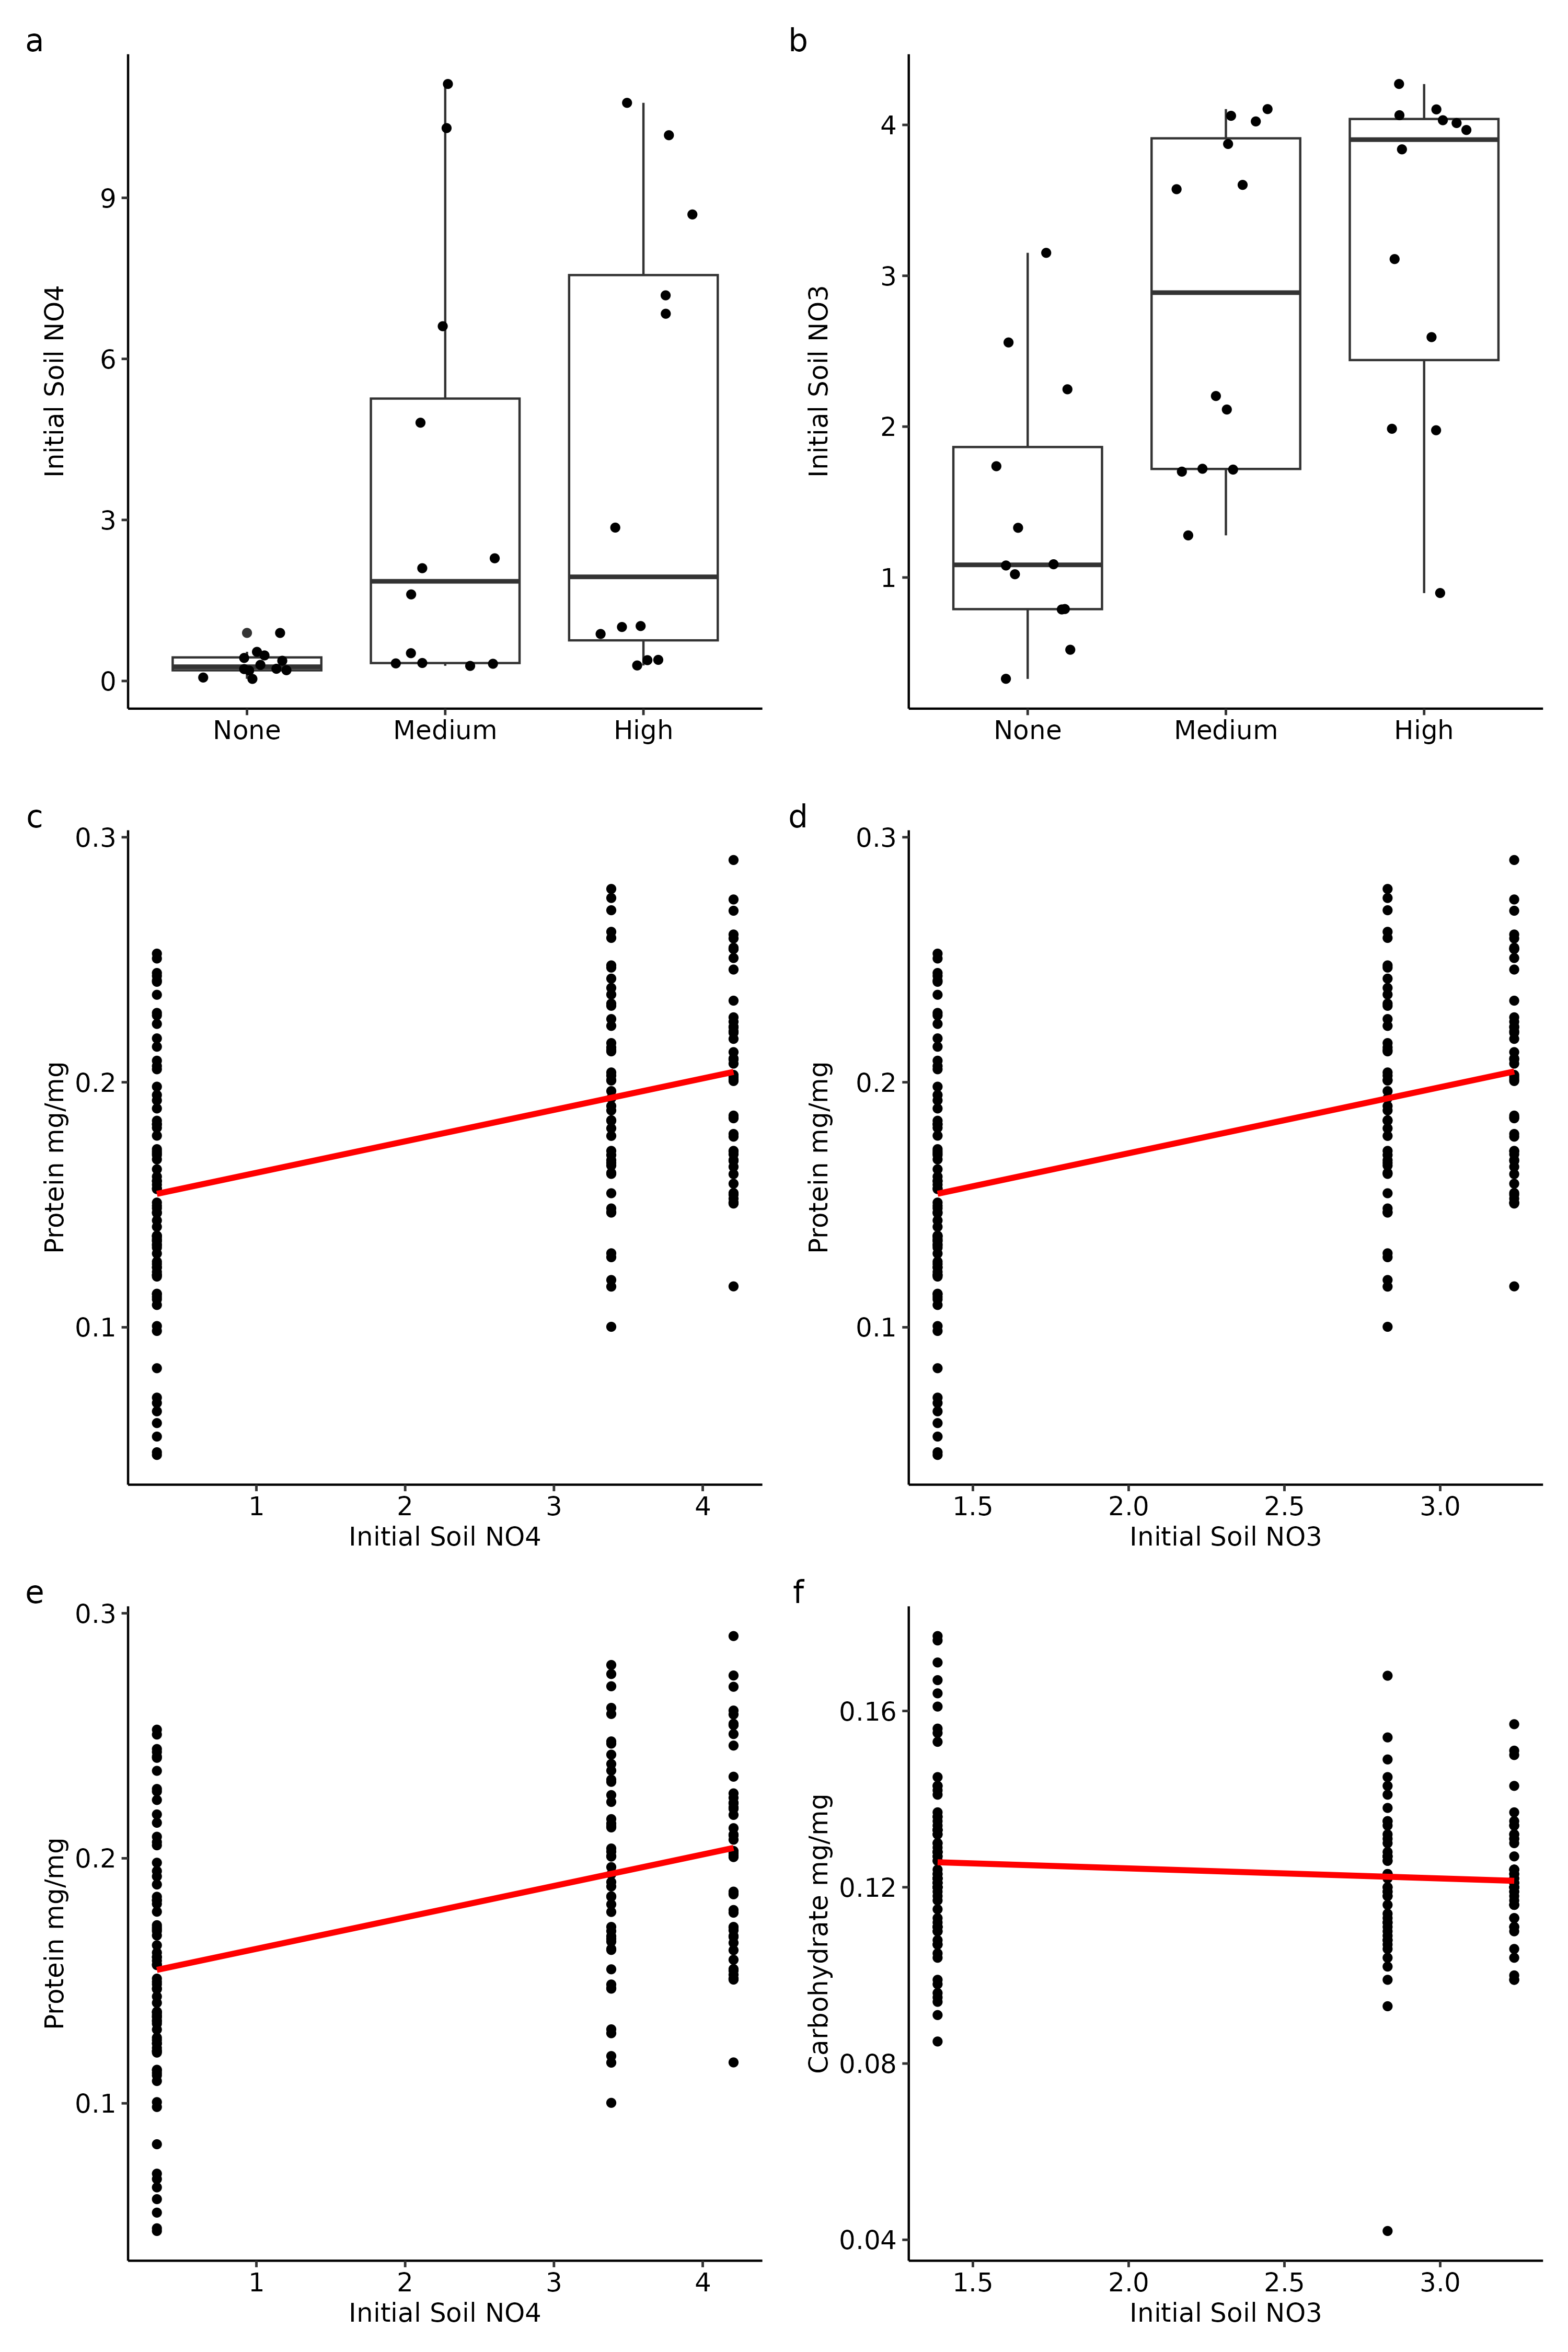
\includegraphics[width=0.8\linewidth,height=\textheight,keepaspectratio]{output/publication_figures/field_cage_plant_and_soil_nutrient_correlations.png}

}

\caption{\label{suppfig-field-cage-plant-soil-nutrient-correlations}Field
cage soil nitrogen content by treatment (A \& B) and regressed with
plant carbohydrates and protein (C-F).}

\end{suppfig}%

\begin{suppfig}

\centering{

\pandocbounded{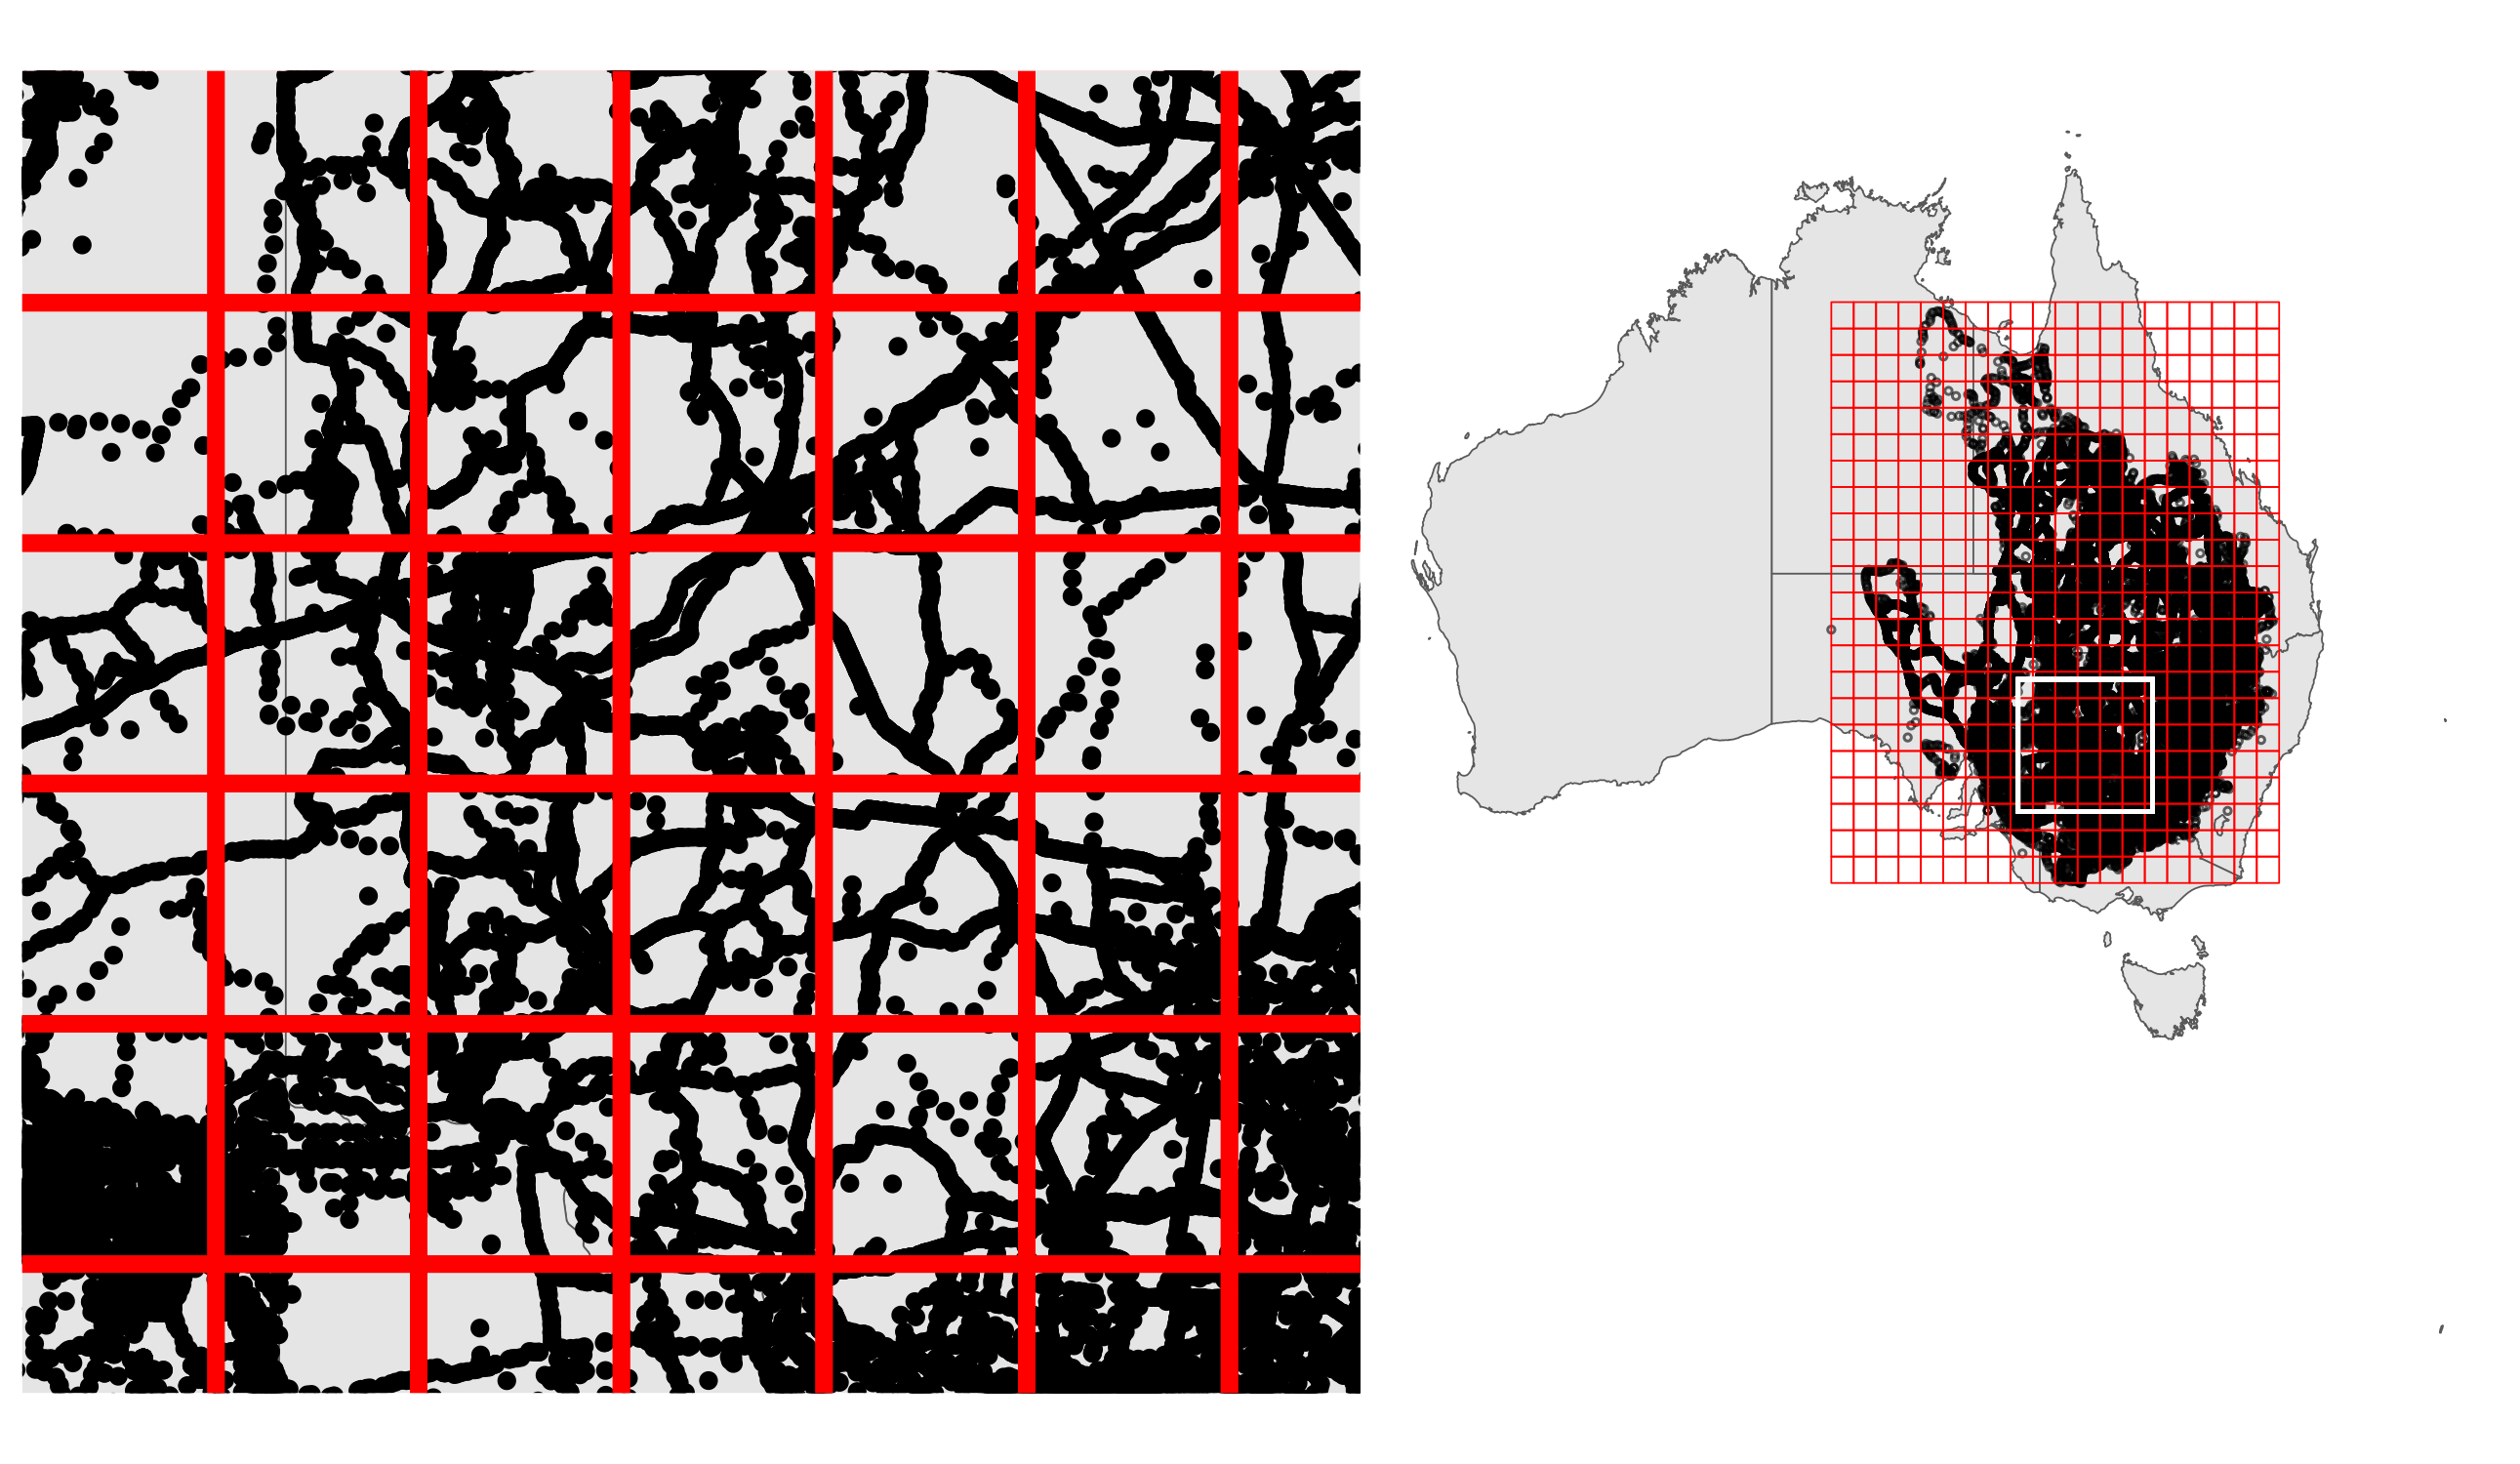
\includegraphics[keepaspectratio]{output/publication_figures/spatial_modeling_grid_example_map.png}}

}

\caption{\label{suppfig-grid-example}Map illustrating the summarization
of point observation data into a fishnet grid across eastern Australia.
The inset map location is represented by the white box. We summed the
number of outbreak, nil, and total observations. The grid in this figure
is not at a 1 km\textsuperscript{2} scale for demonstration purposes, as
the cells would be too small to see.}

\end{suppfig}%

\begin{suppfig}

\centering{

\pandocbounded{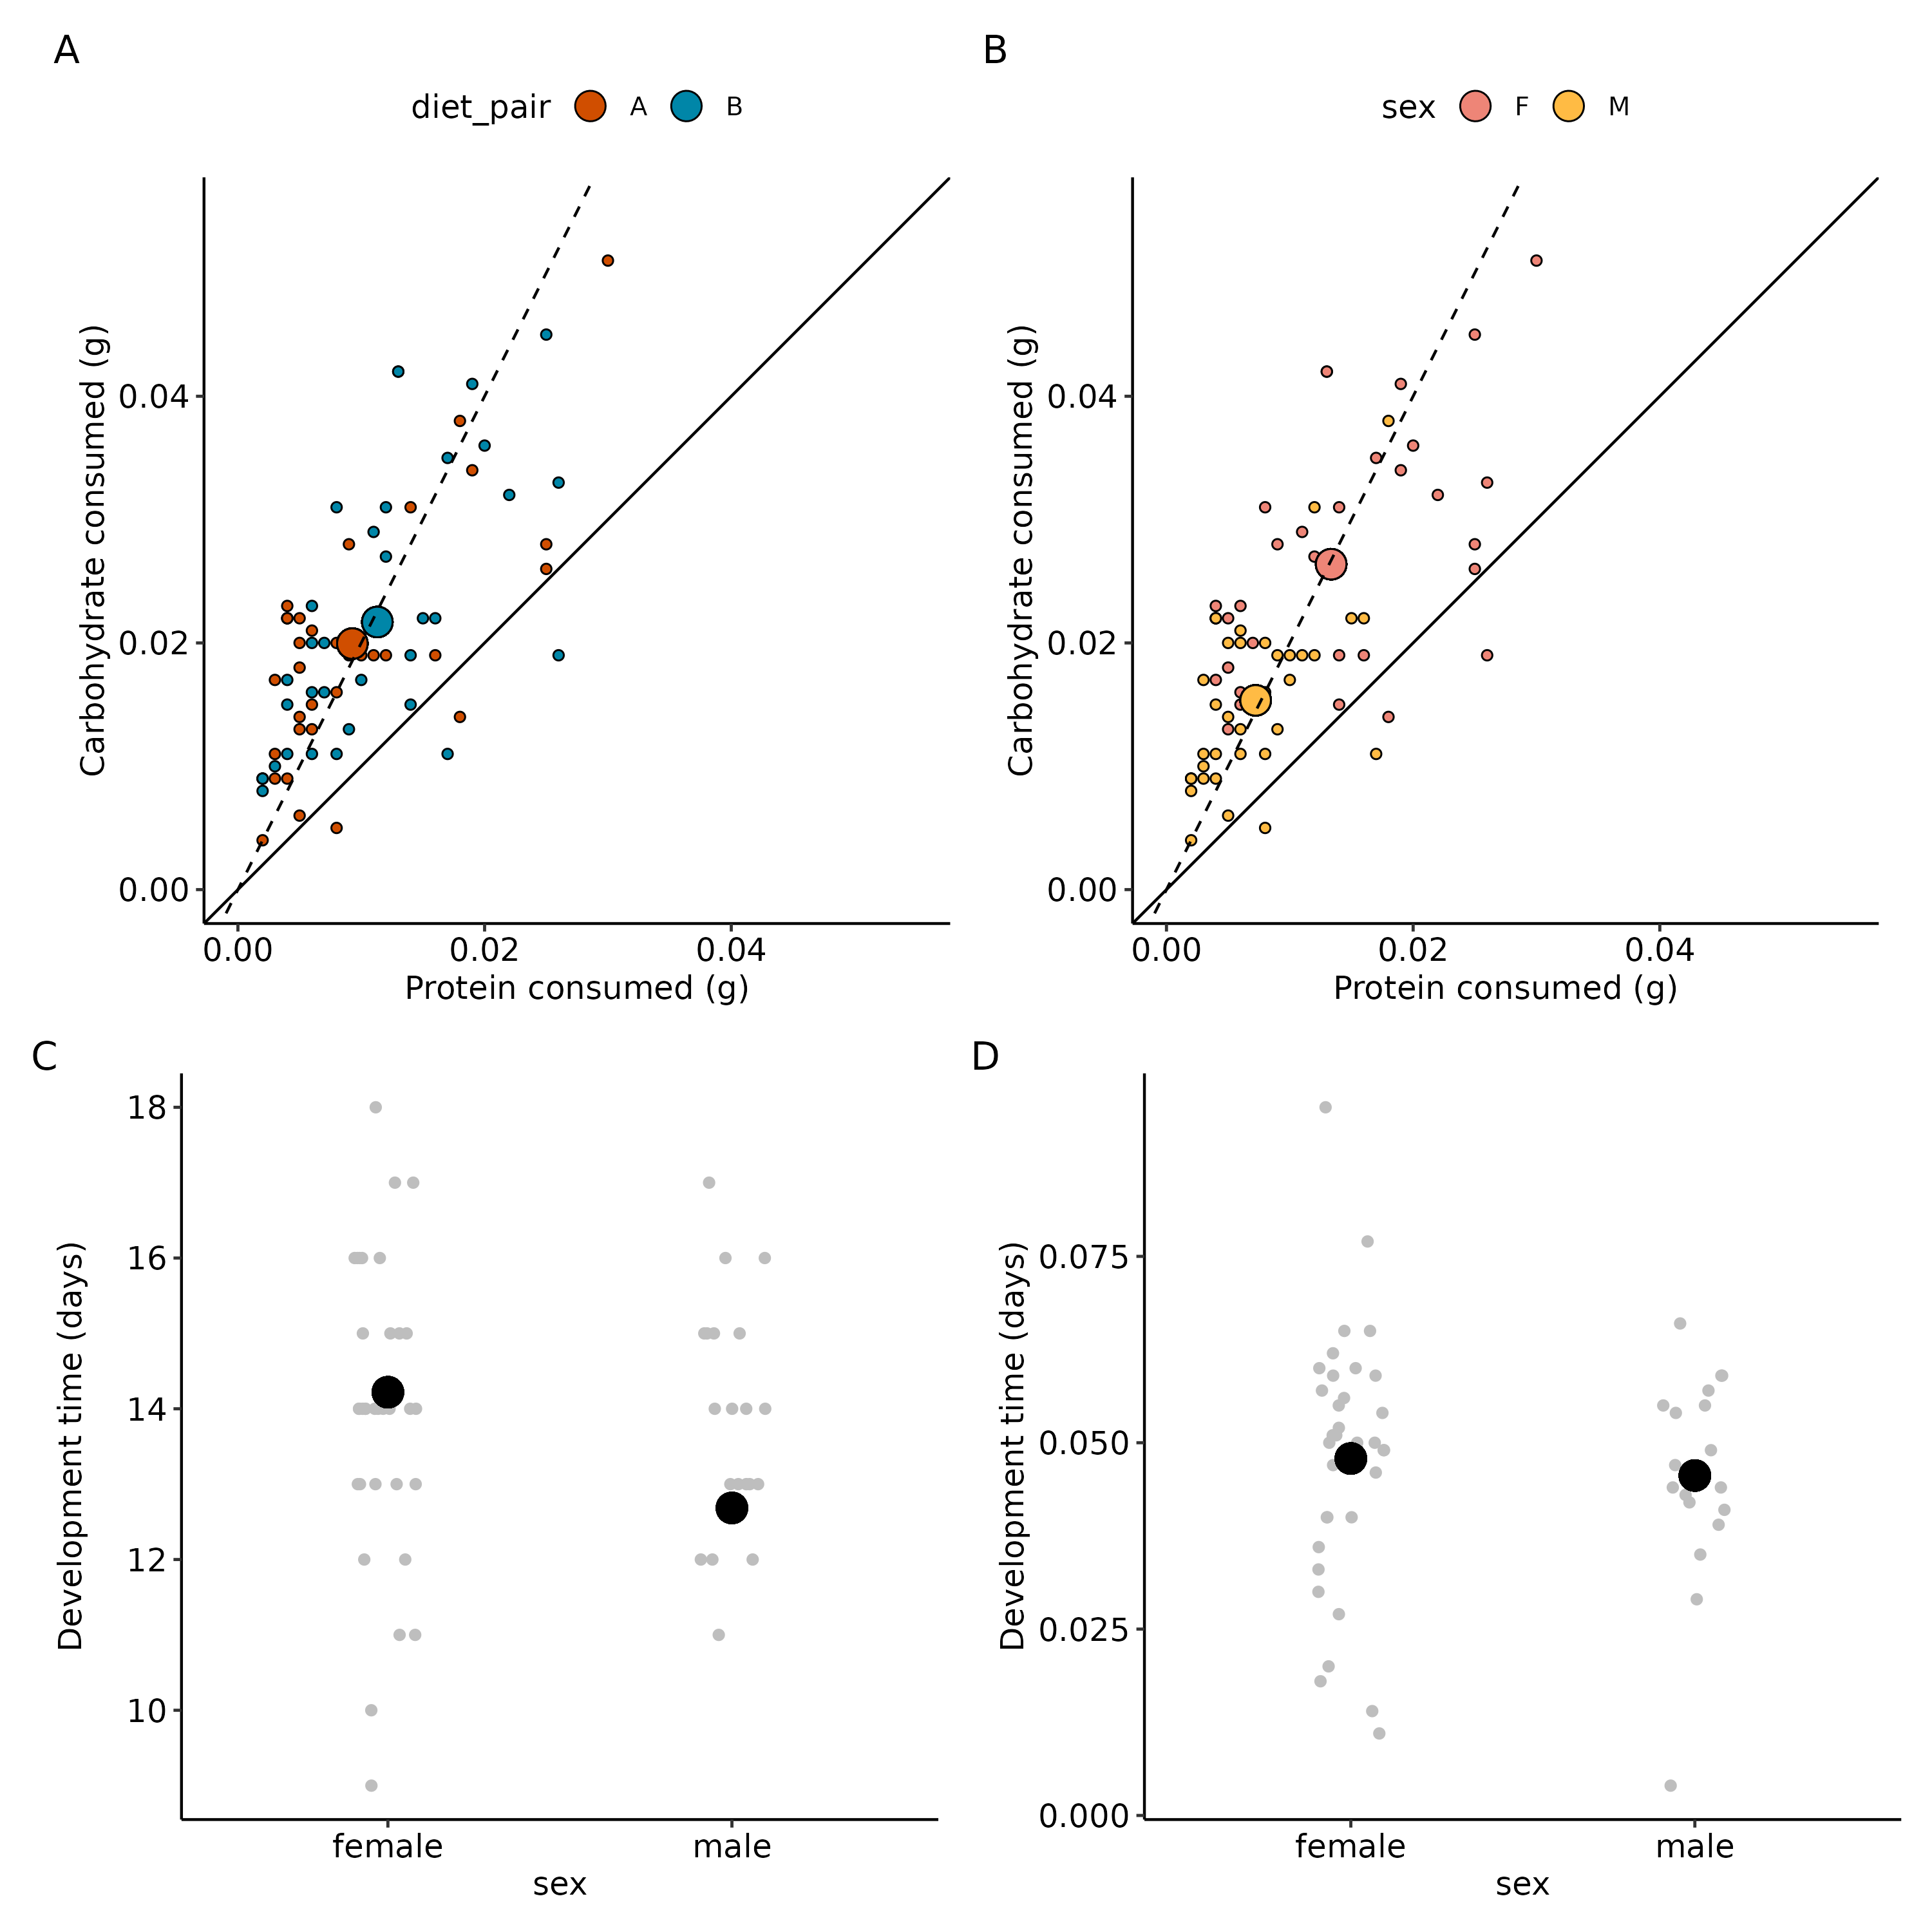
\includegraphics[keepaspectratio]{output/publication_figures/supplement_figure_3.png}}

}

\caption{\label{suppfig-field-pop-nutrients}Nutrient consumption for
outbreaking field populations of \emph{C. terminifera} by diet pair (A)
and sex (B) and development time (C) specific growth rate (D) by sex.
The P:C ratio did not differ between diet pairing and sex. Females
consumed more diet (but kept the same ratio) than males. Big circles
represent estimated marginal means from the model while little circles
represent raw data.}

\end{suppfig}%

\begin{suppfig}

\centering{

\pandocbounded{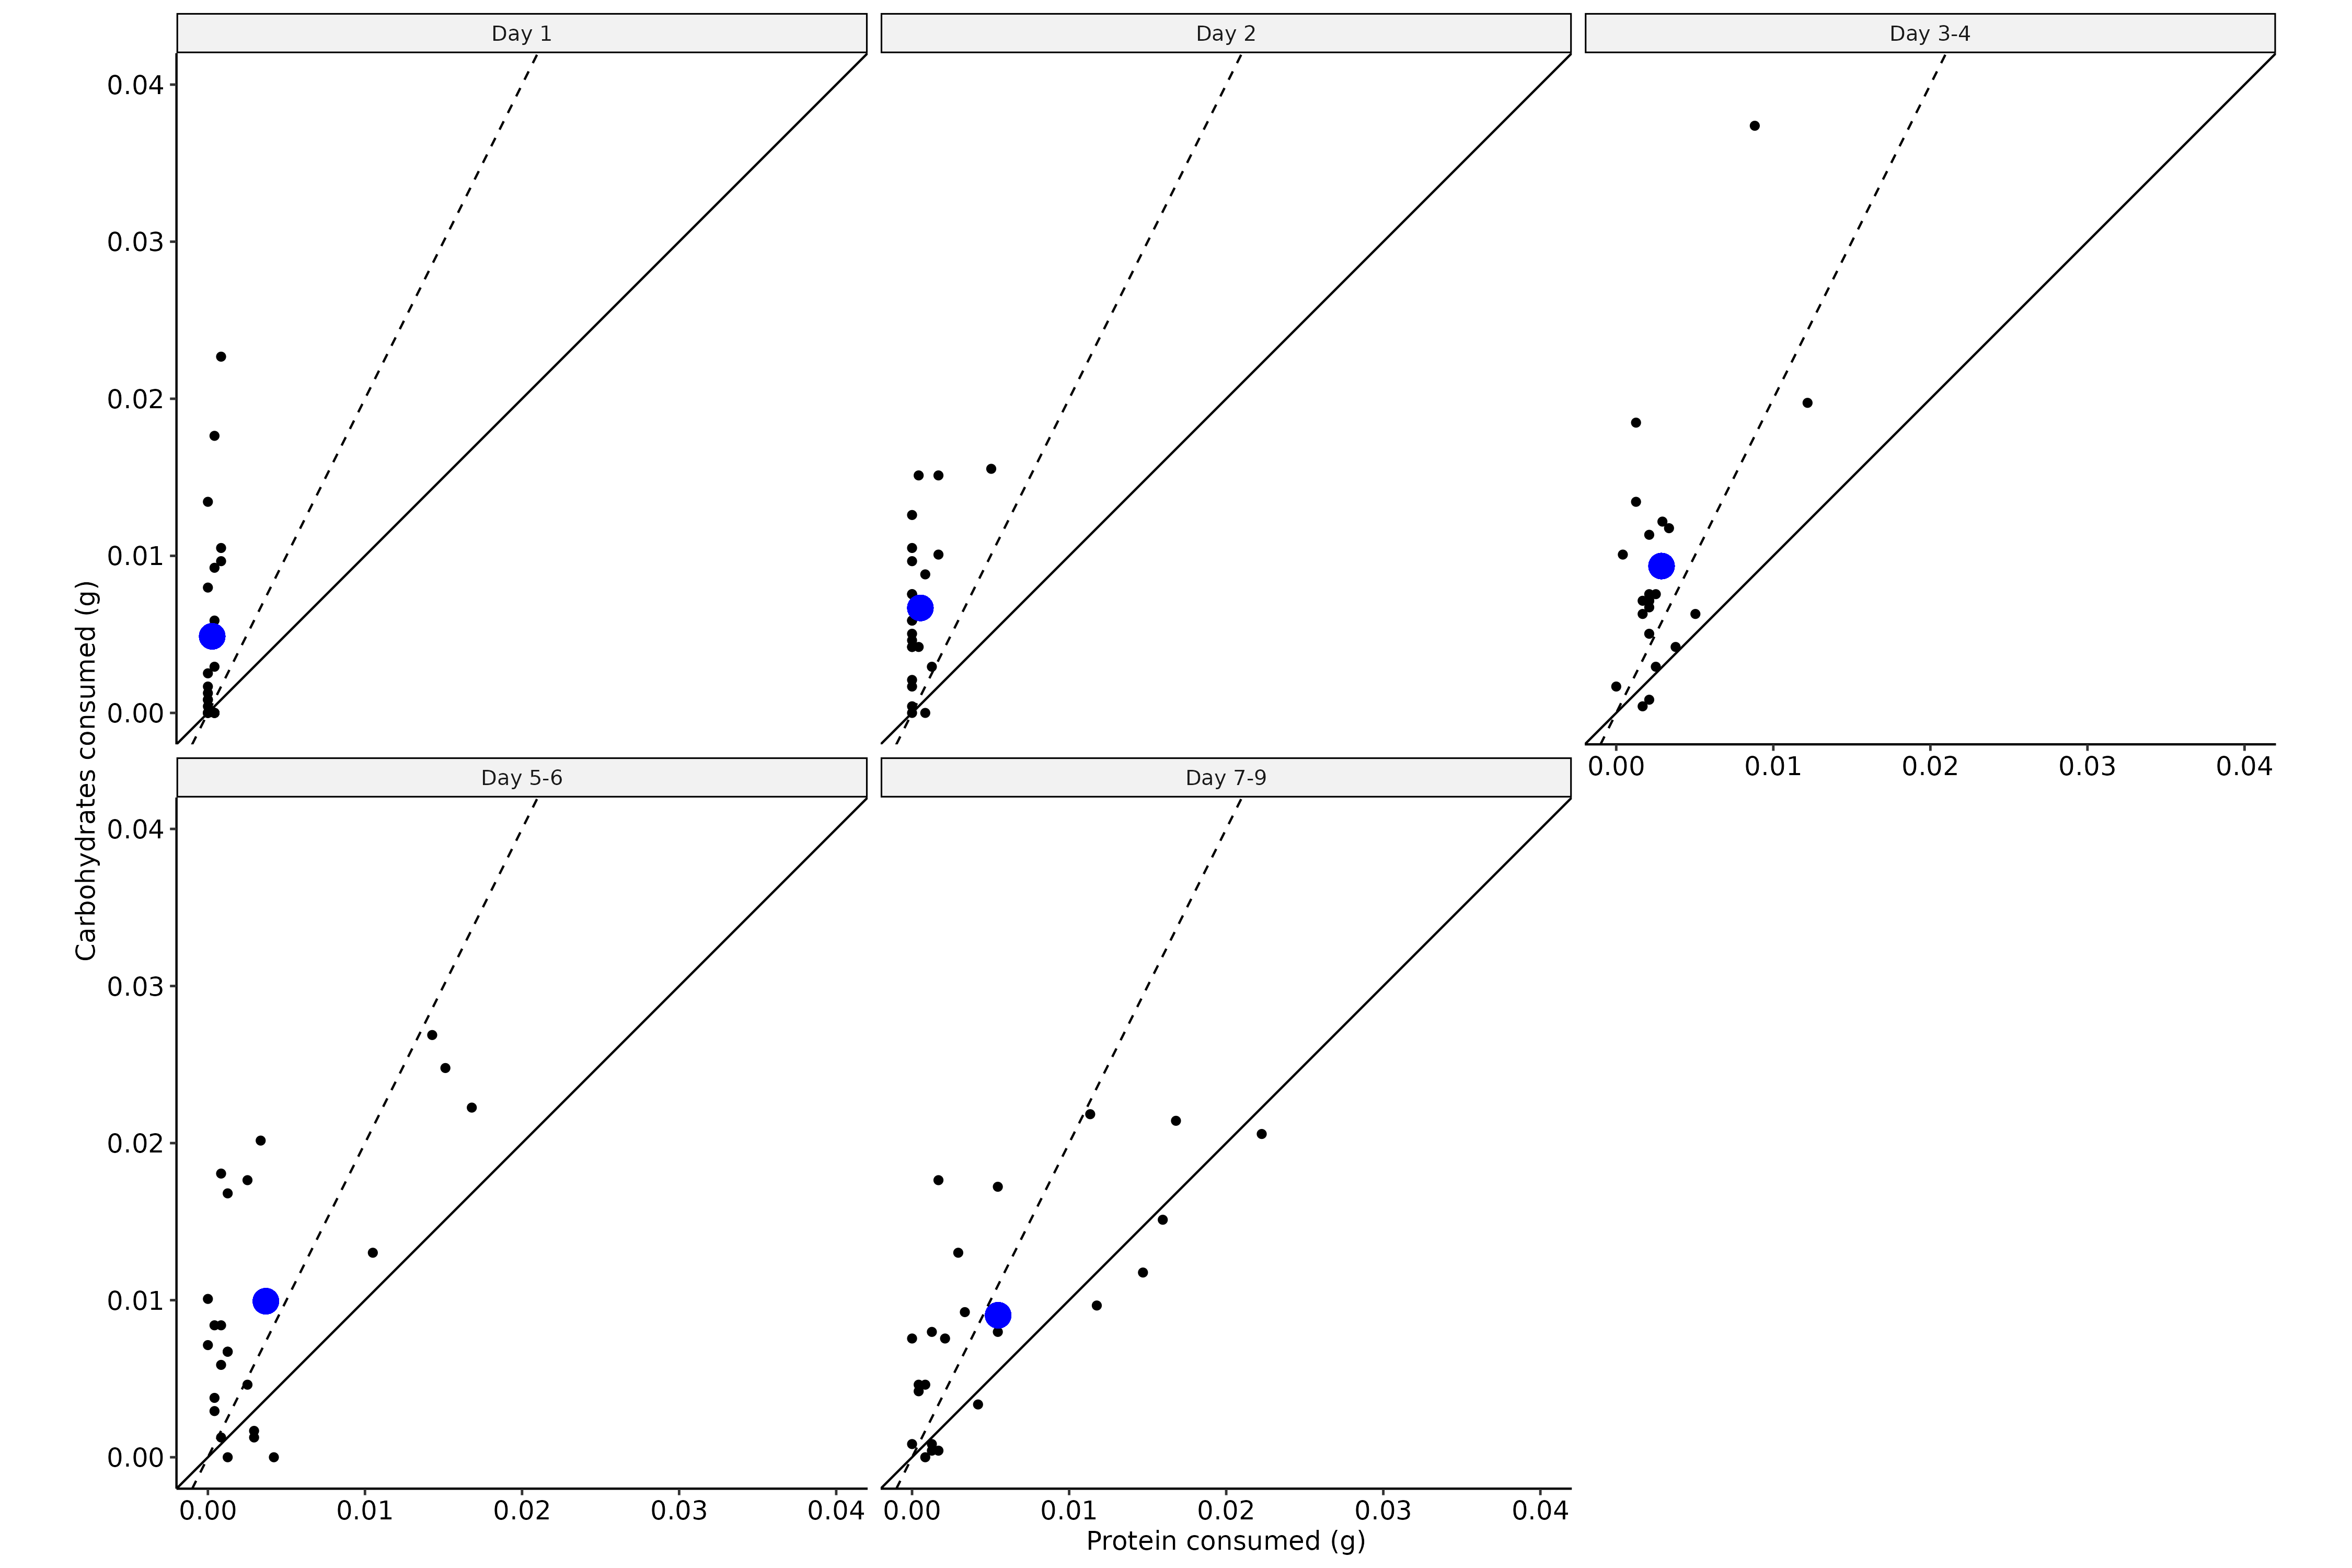
\includegraphics[keepaspectratio]{output/publication_figures/field_cage_locust_intake_rebalance_day_facet_plot.png}}

}

\caption{\label{suppfig-field-cage-rebalancing-facet}Individual time
step intake targets for grasshoppers kept in both high nitrogen
fertilization and control cages. Blue dots represent estimated marginal
means from the model while blacks dots represent raw individual intake
targets.}

\end{suppfig}%

\begin{suppfig}

\centering{

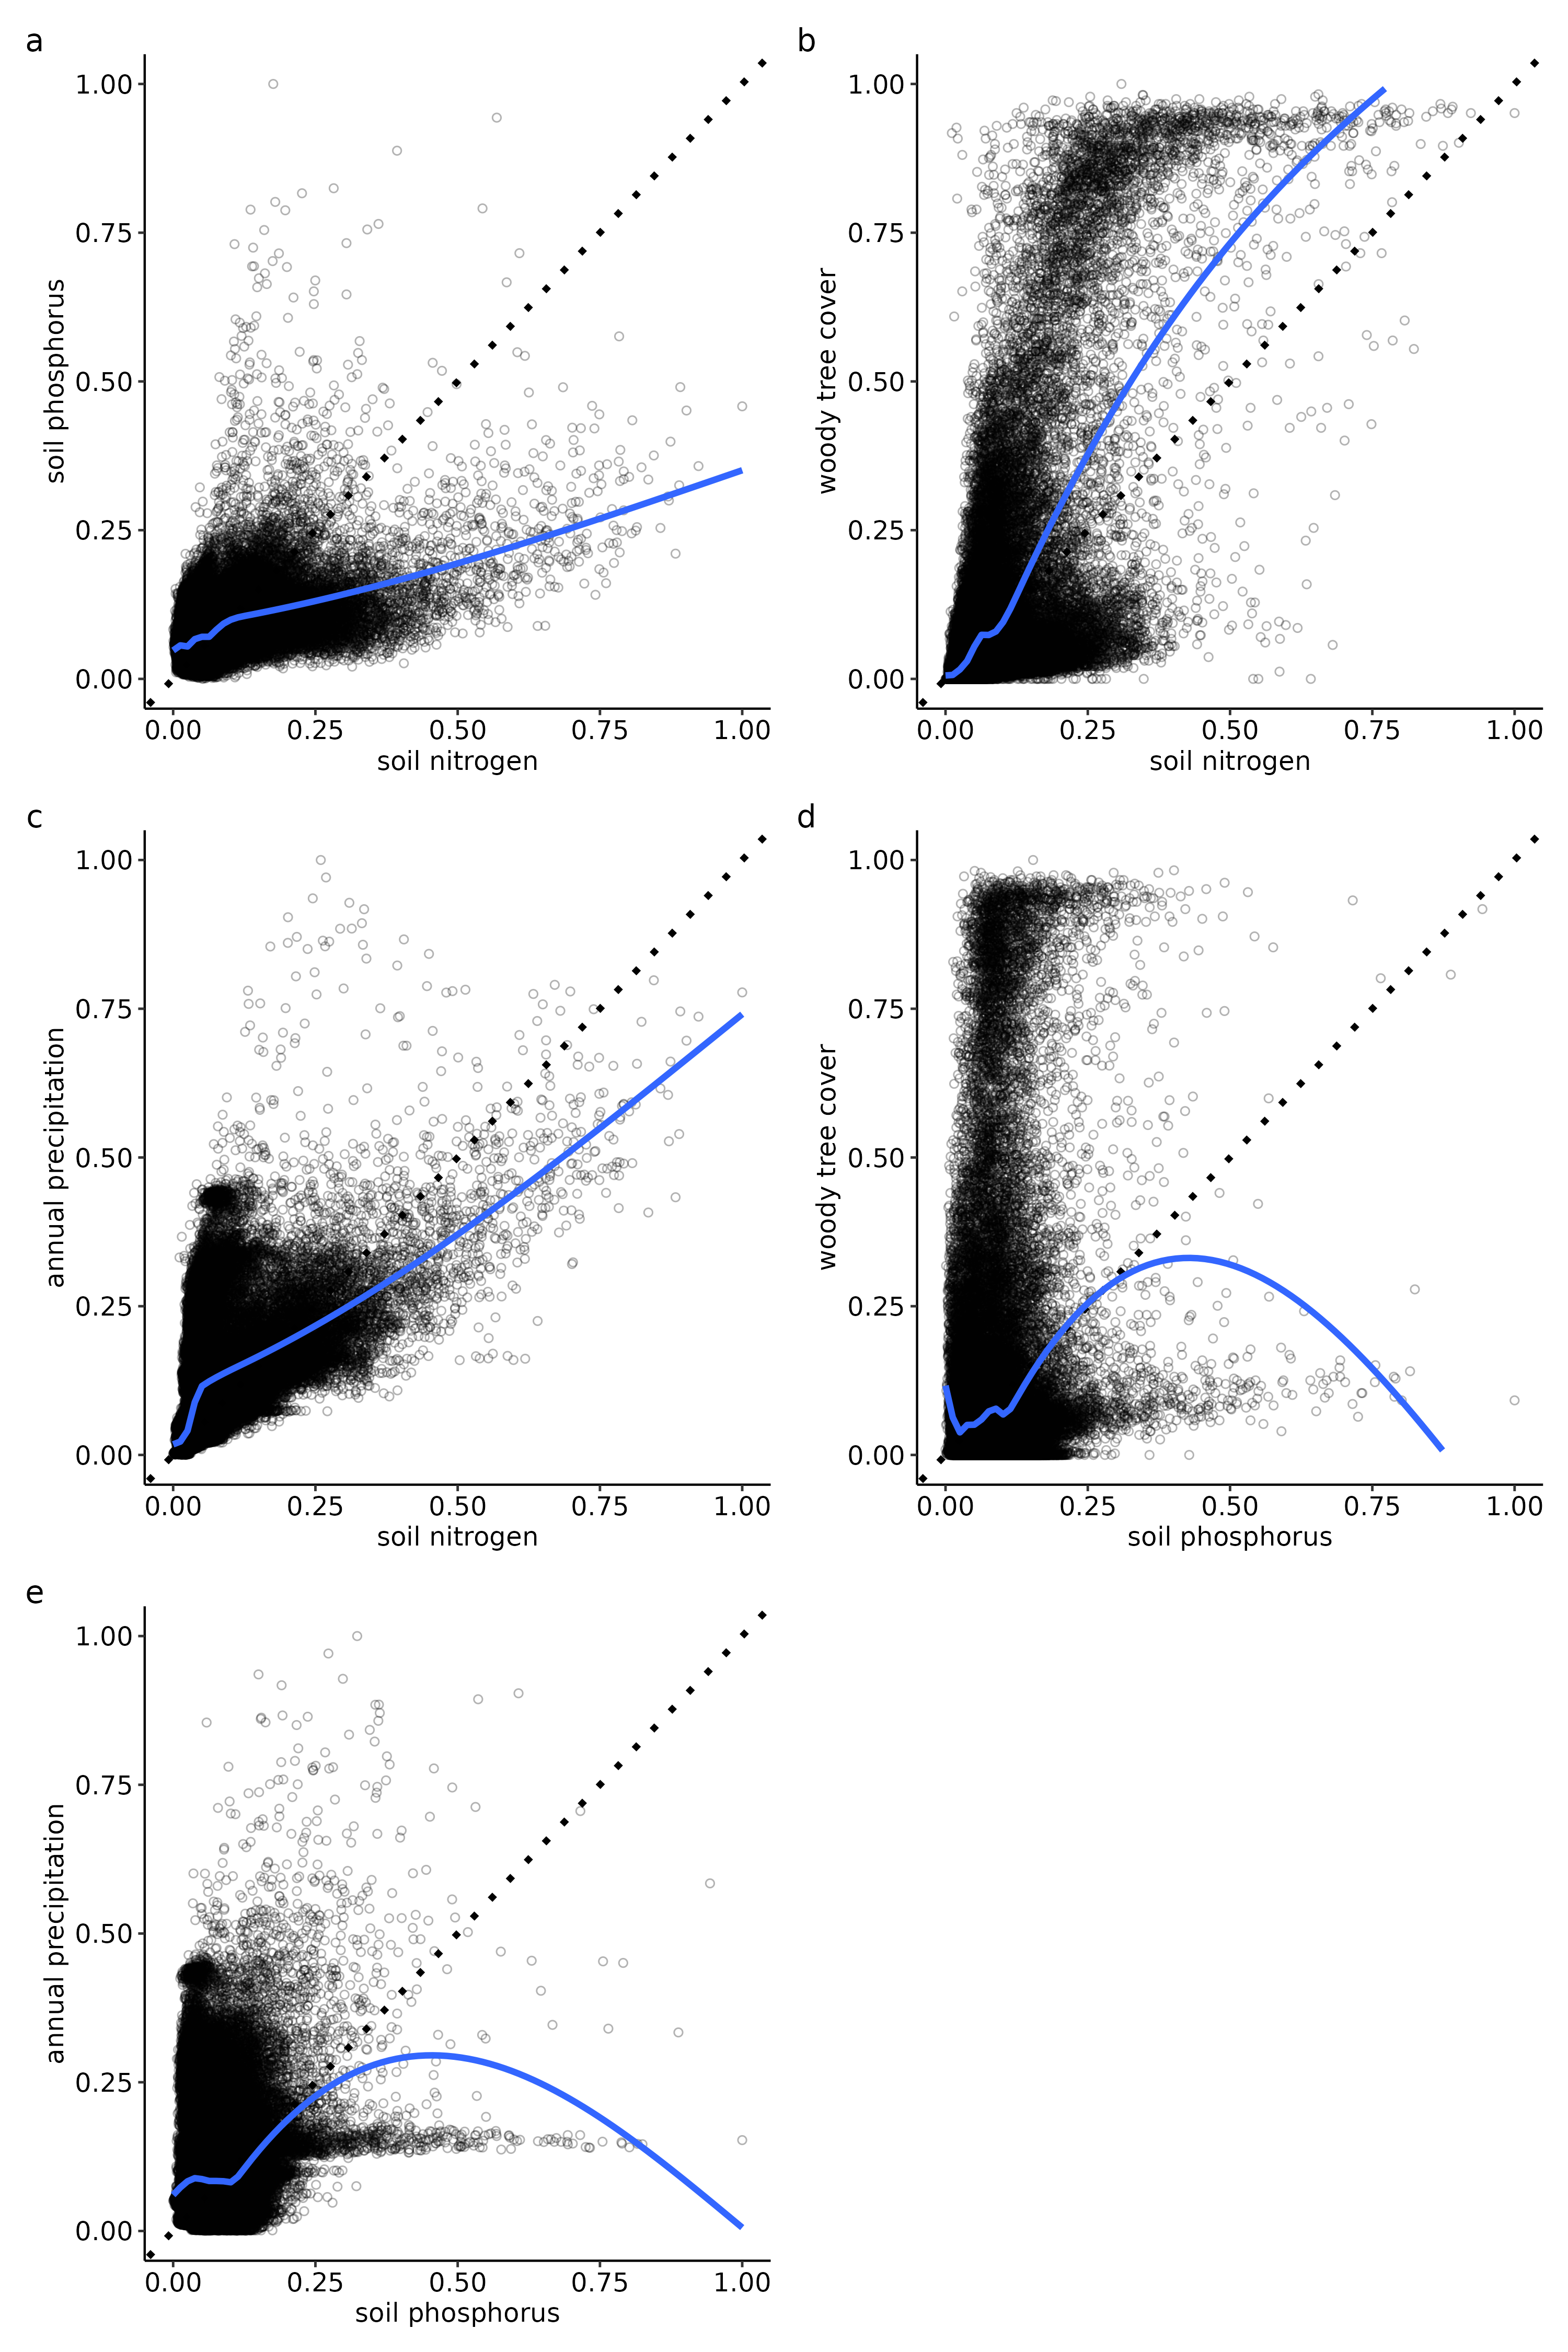
\includegraphics[width=0.8\linewidth,height=\textheight,keepaspectratio]{output/publication_figures/spatial_modeling_environment_correlation_figure.png}

}

\caption{\label{suppfig-spatial-modeling-env-corr}Environmental variable
correlations between mean annual precipitation, soil nitrogen, soil
phosphorus, and woody vegetation pixel coverage. Mean annual
precipitation was sourced from WorldClim V1 Bioclim, soil nitrogen and
phosphorus was sourced from Soil and Landscape Grid of Australia, and
woody vegetation pixel coverage was sourced from Global Forest Cover
Change dataset. We averaged woody coverage for each pixel between the
years 2000 and 2017. For all rasters, we randomly sampled 100,000
georeferenced points and extracted values. All values have been scaled
and min-max normalized (to fall within 0-1) for visual clarity
otherwise, unit scales would mask relationships. Dashed line represents
a 1:1 slope and the blue line is a cubic spline with 10 knots.}

\end{suppfig}%

\begin{suppfig}

\centering{

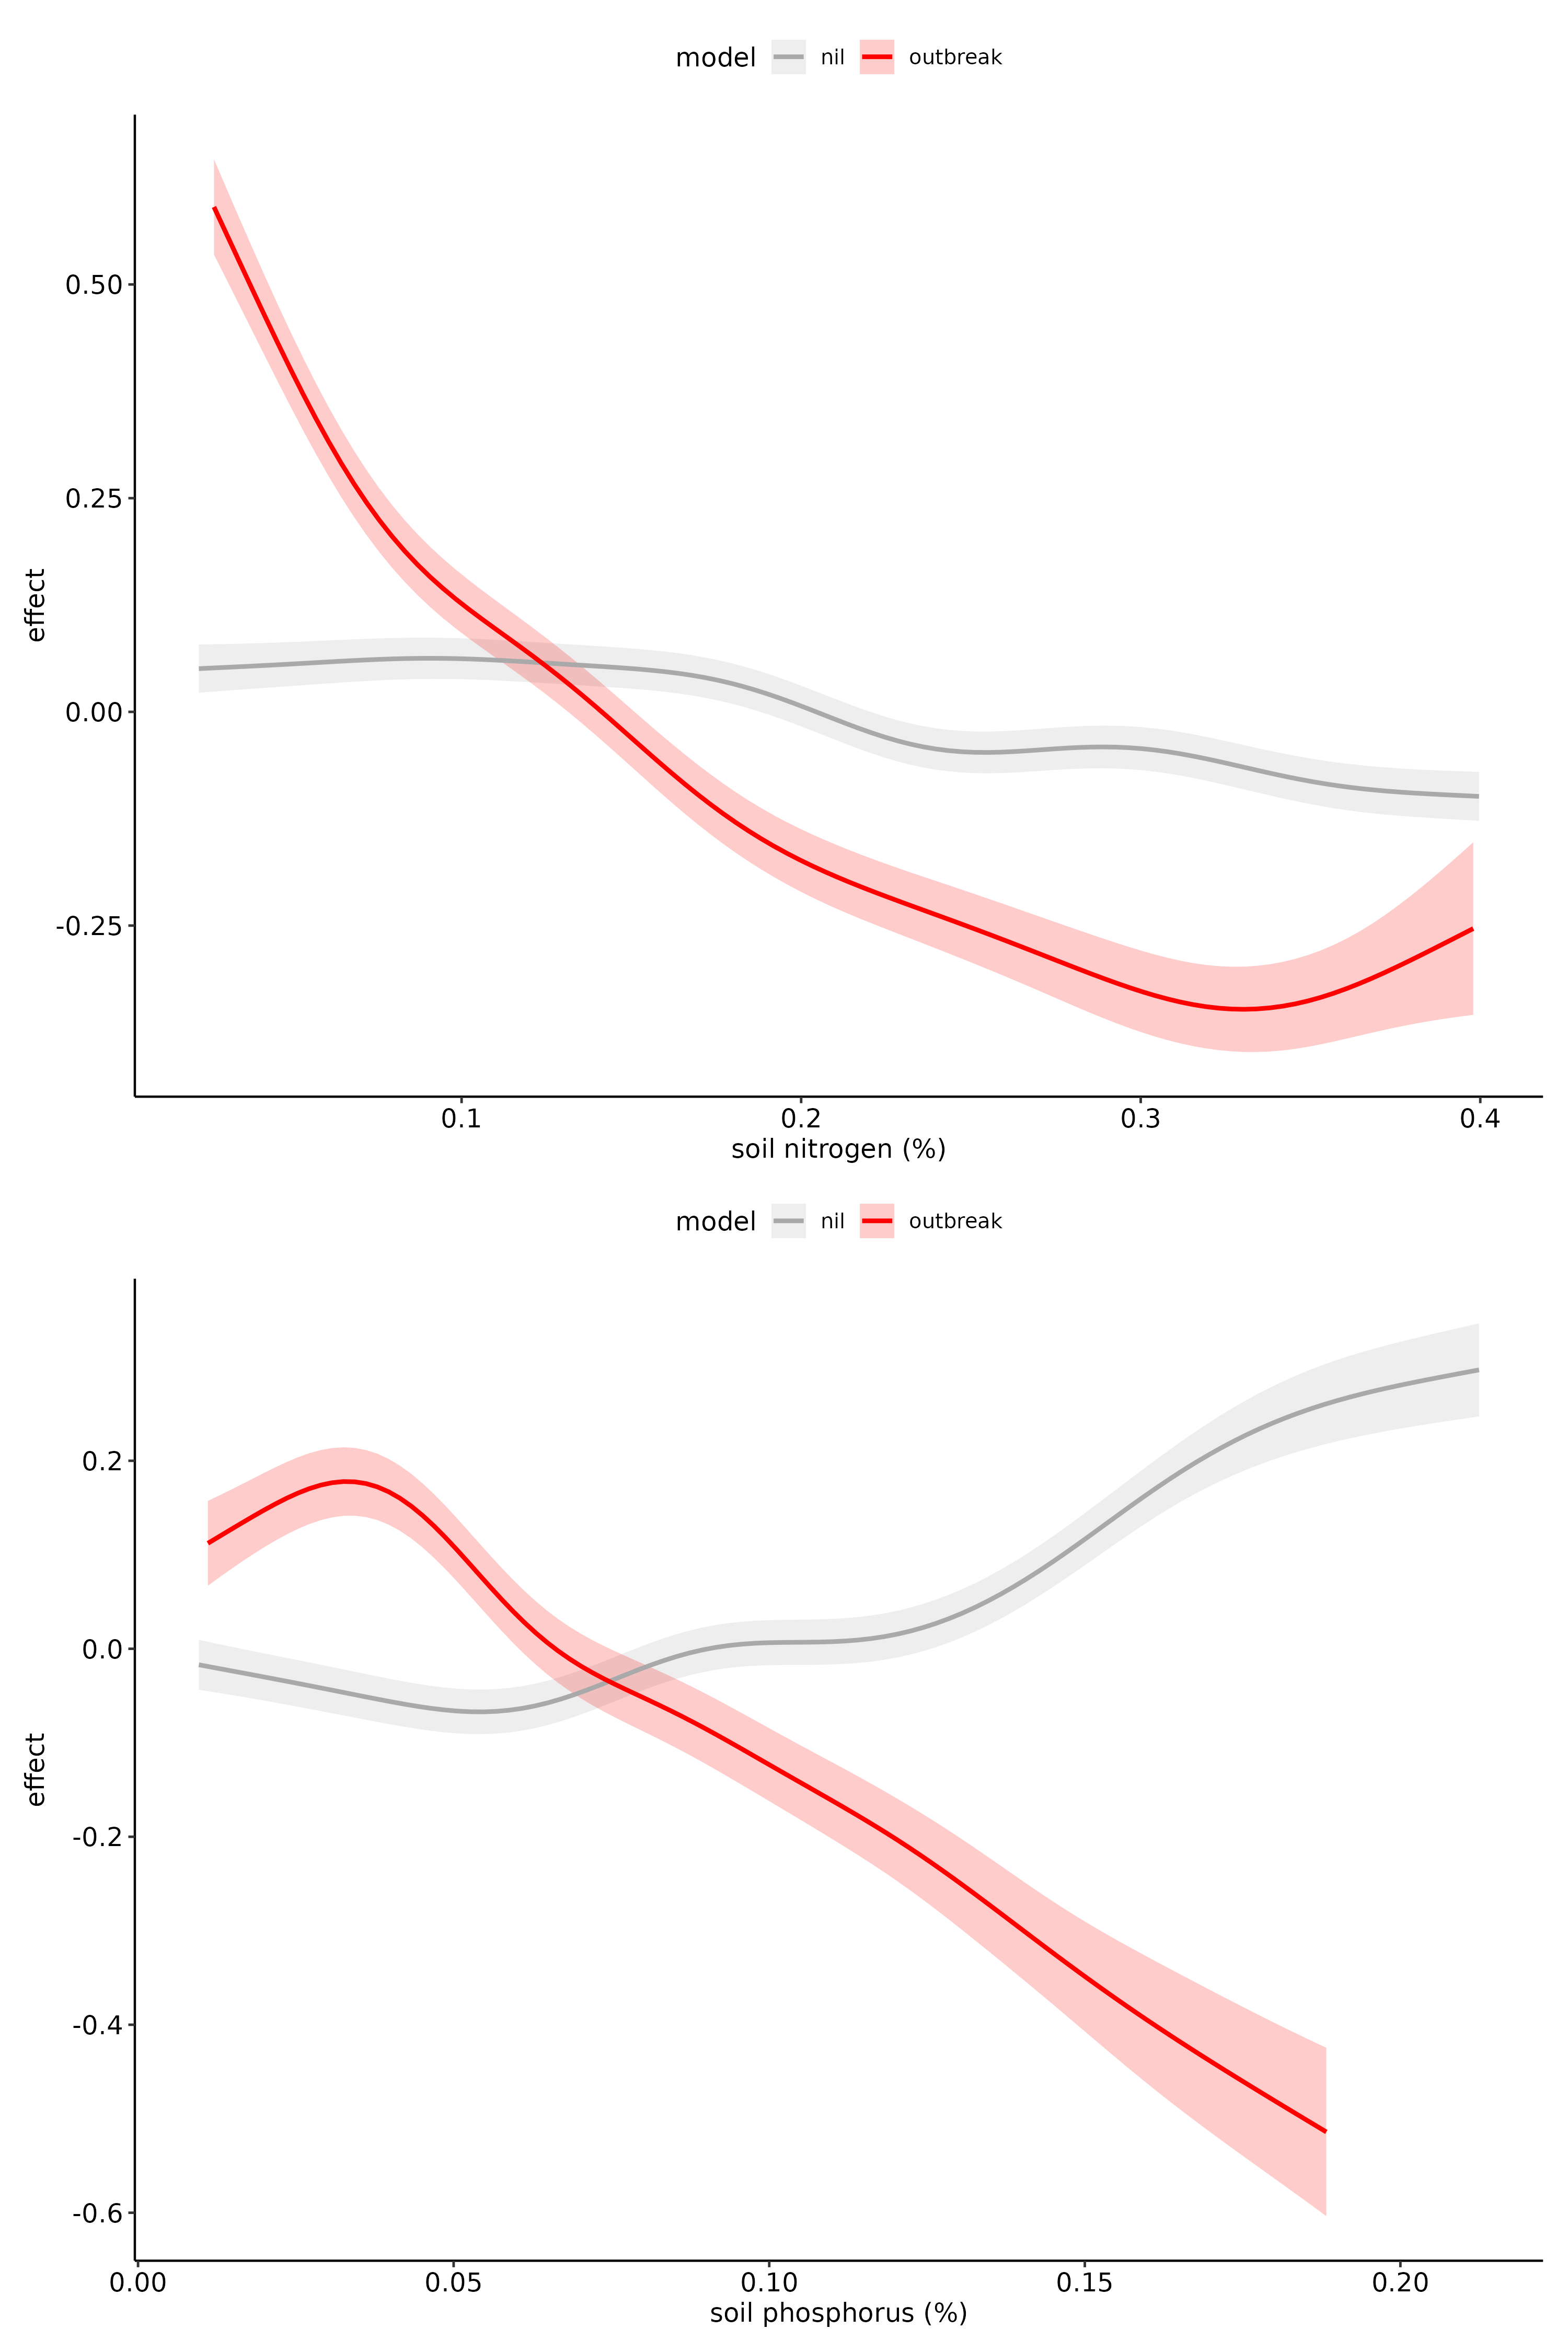
\includegraphics[width=0.8\linewidth,height=\textheight,keepaspectratio]{output/publication_figures/spatial_modeling_outbreak_all_model_variables.png}

}

\caption{\label{suppfig-spatial-modeling-outbreak-all-vars}Historical
outbreaks record survey data modeling with soil nitrogen and
phosphorus.}

\end{suppfig}%

\begin{suppfig}

\centering{

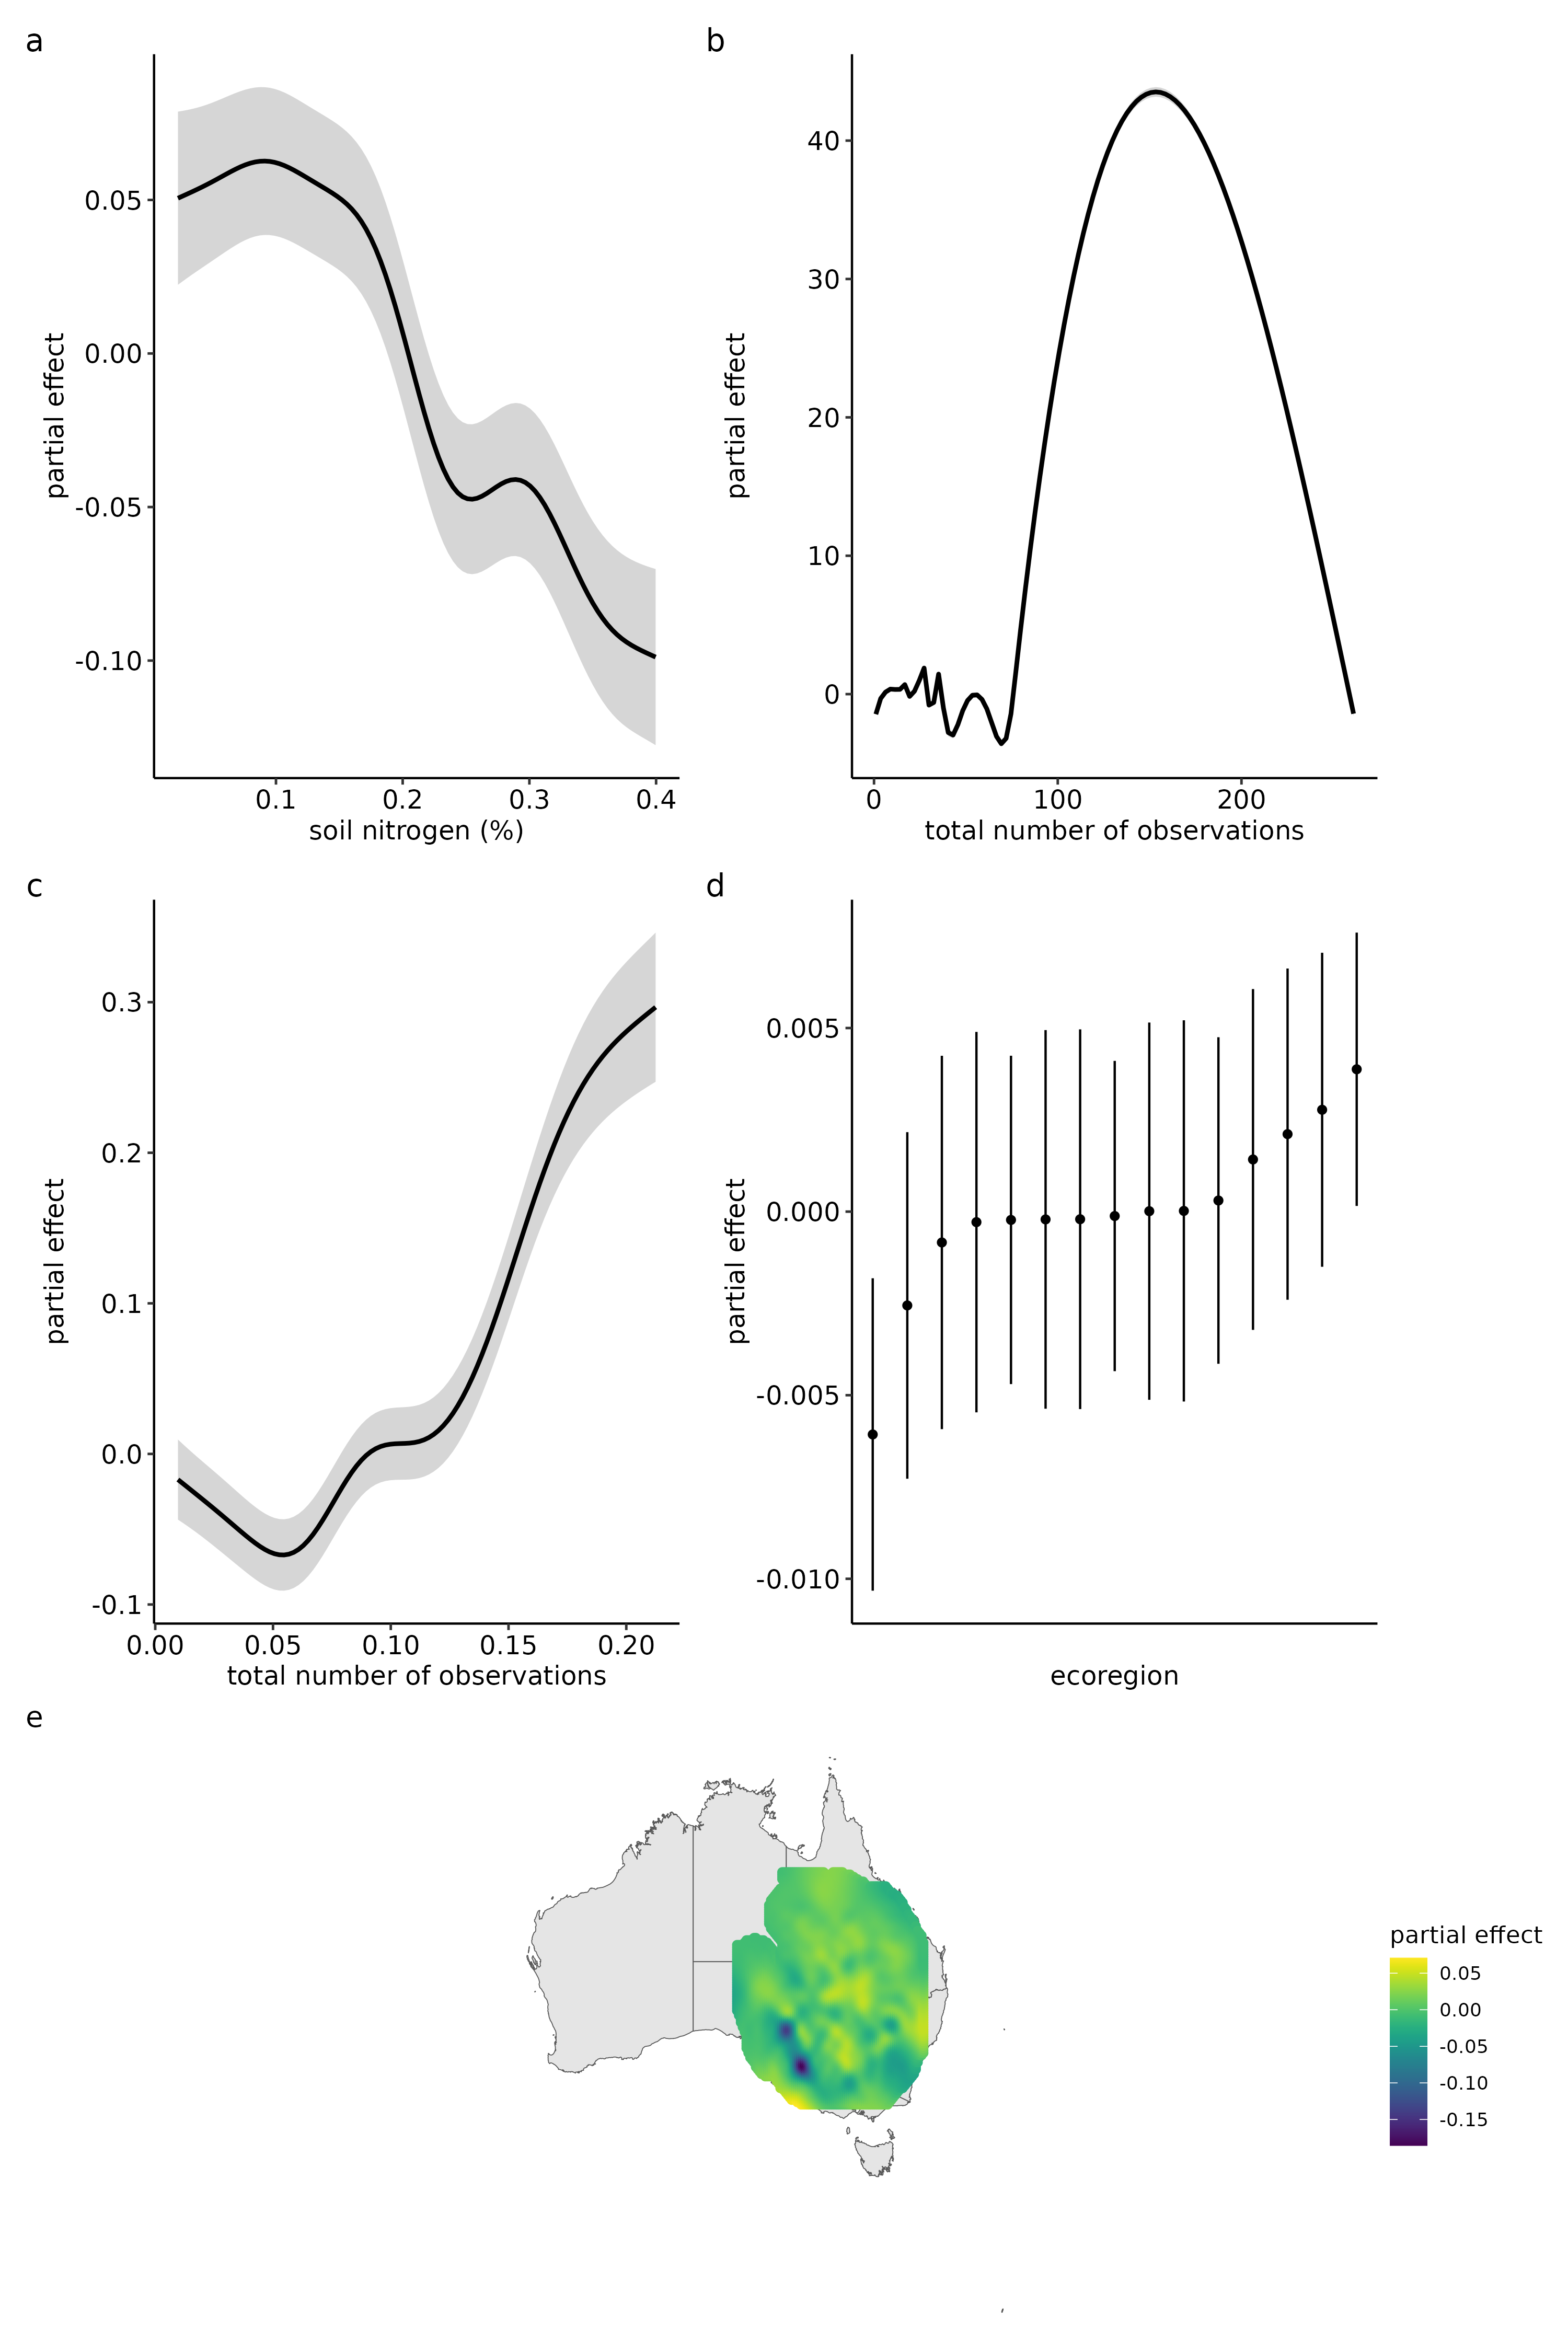
\includegraphics[width=0.8\linewidth,height=\textheight,keepaspectratio]{output/publication_figures/spatial_modeling_nil_all_model_variables.png}

}

\caption{\label{suppfig-spatial-modeling-nil-all-vars}Historical nil
record survey data modeling with soil nitrogen and phosphorus.}

\end{suppfig}%

\begin{suppfig}

\centering{

\pandocbounded{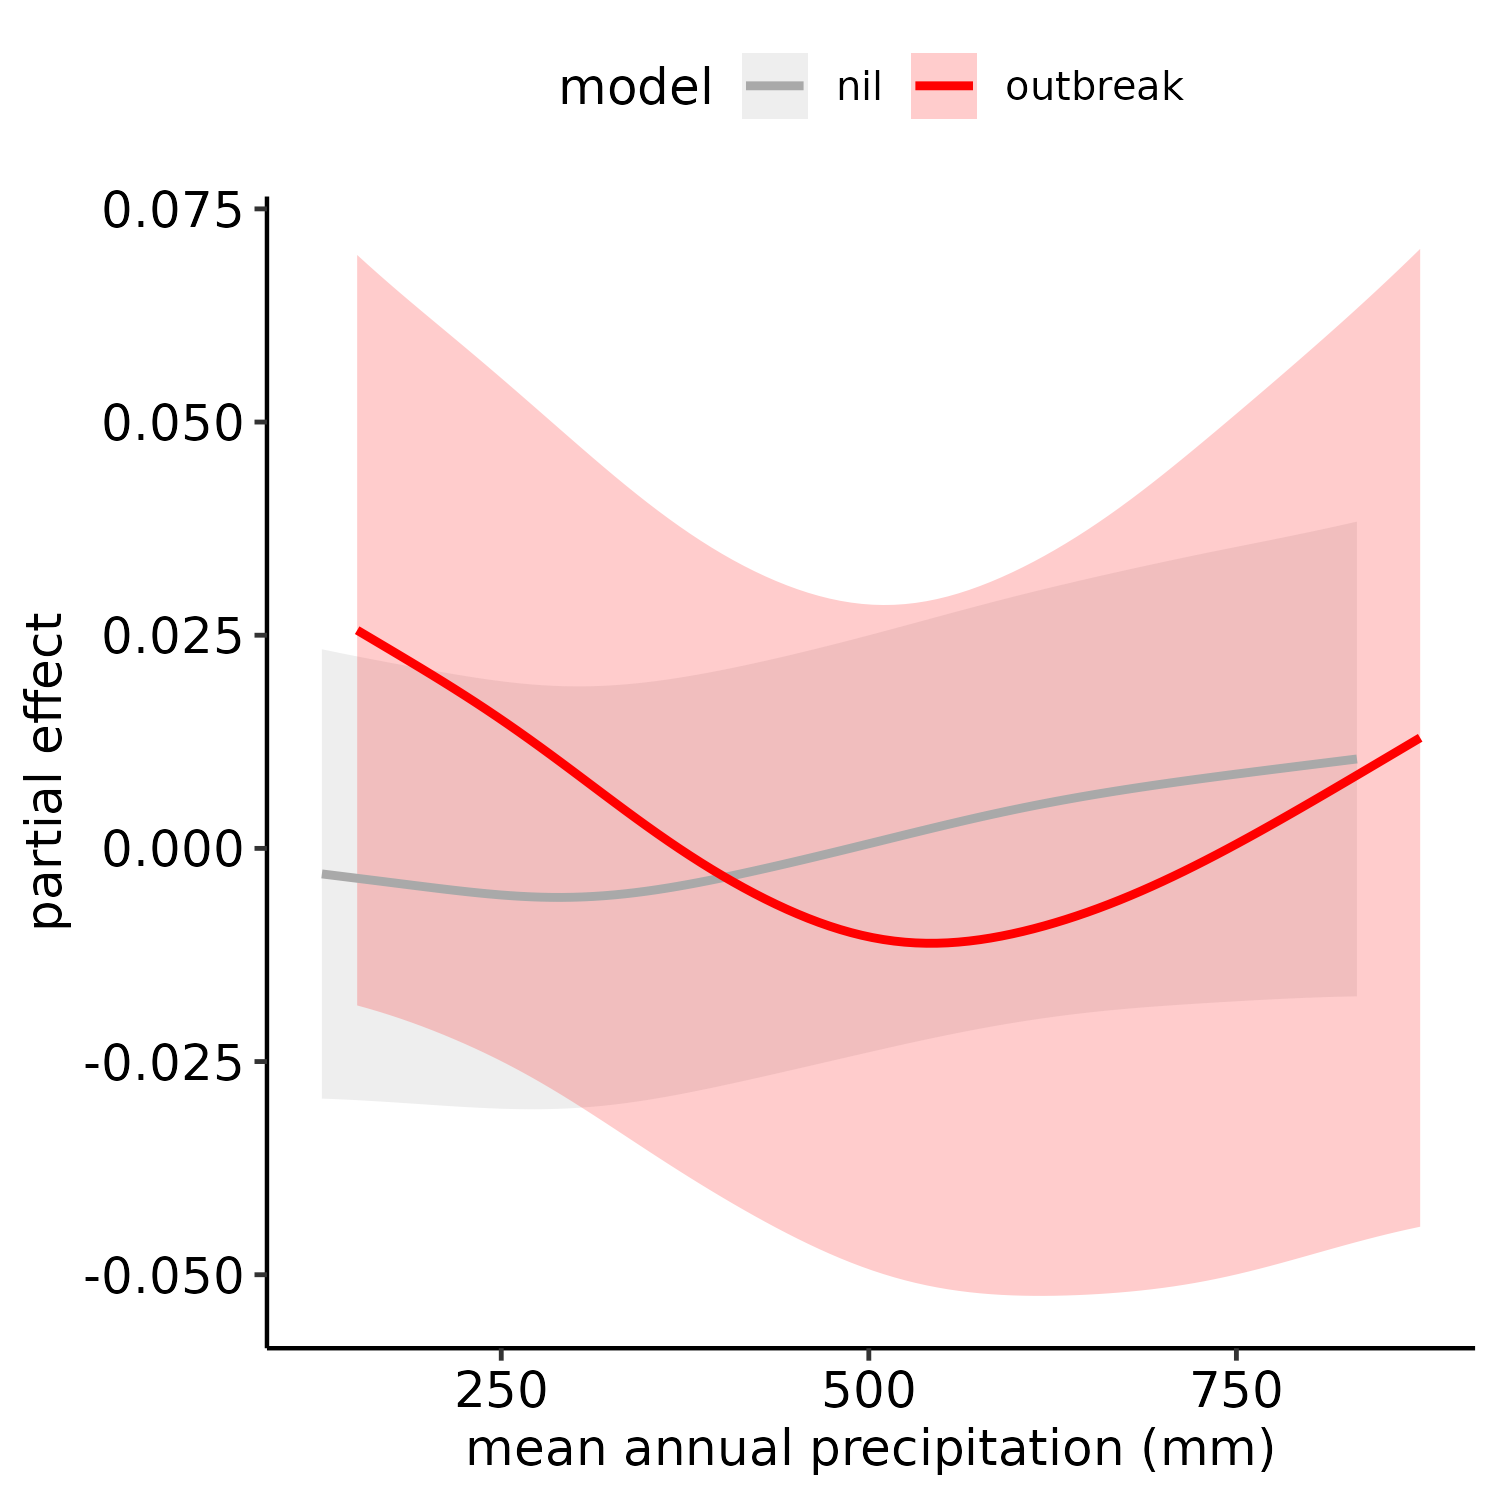
\includegraphics[keepaspectratio]{output/publication_figures/spatial_modeling_locust_outbreak_with_map.png}}

}

\caption{\label{suppfig-spatial-modeling-map-outbreak-corr}The
relationship between locust outbreaks and nil observations and mean
annual precipitation. This is included as a visual comparison for the
soil nitrogen relationship seen in
Figure~\ref{fig-spatial-model-nto-pto}}

\end{suppfig}%

\blandscape

\begin{supptbl}

\centering{

\begingroup
\setlength\LTleft{0.05\linewidth}
\setlength\LTright{0.05\linewidth}\fontsize{8.2pt}{9.9pt}\selectfont
\begin{longtable*}{@{\extracolsep{\fill}}llrrrrrrr}
\toprule
treatment & species & date & Plant C mg/mg & Plant N & Plant P mg/mg & Plant Carb mg/mg & Soil NO3 mg/L & Soil NO4 mg/L \\ 
\midrule\addlinespace[2.5pt]
High & {\itshape Digitaria spp.} & 2015-12-01 & 0.419 & 0.027 & 0.182 & 0.108 & 3.238 & 4.207 \\ 
 & {\itshape Enteropogon spp.} & 2015-11-11 & 0.425 & 0.030 & 0.199 & 0.128 &  &  \\ 
 & {\itshape Enteropogon spp.} & 2015-11-25 & 0.414 & 0.028 & 0.180 & 0.120 &  &  \\ 
 & {\itshape Enteropogon spp.} & 2015-12-01 & 0.414 & 0.024 & 0.163 & 0.125 &  &  \\ 
 & {\itshape Cyperus spp.} & 2015-11-11 & 0.423 & 0.030 & 0.228 & 0.125 &  &  \\ 
 & {\itshape Cyperus spp.} & 2015-11-25 & 0.415 & 0.032 & 0.220 & 0.131 &  &  \\ 
 & {\itshape Cyperus spp.} & 2015-12-01 & 0.417 & 0.027 & 0.227 & 0.126 &  &  \\ 
 & {\itshape Plaspladium spp.} & 2015-12-01 & 0.400 & 0.029 & 0.233 & 0.120 &  &  \\ 
 & {\itshape Rytidosperma spp.} & 2015-11-11 & 0.424 & 0.023 & 0.206 & 0.125 &  &  \\ 
 & {\itshape Rytidosperma spp.} & 2015-11-25 & 0.422 & 0.029 & 0.243 & 0.112 &  &  \\ 
 & {\itshape Rytidosperma spp.} & 2015-12-01 & 0.419 & 0.025 & 0.217 & 0.117 &  &  \\ 
Medium & {\itshape Enteropogon spp.} & 2015-11-11 & 0.431 & 0.042 & 0.209 & 0.126 & 2.831 & 3.385 \\ 
 & {\itshape Enteropogon spp.} & 2015-11-25 & 0.417 & 0.026 & 0.210 & 0.137 &  &  \\ 
 & {\itshape Enteropogon spp.} & 2015-12-01 & 0.415 & 0.022 & 0.146 & 0.124 &  &  \\ 
 & {\itshape Cyperus spp.} & 2015-11-11 & 0.424 & 0.038 & 0.213 & 0.119 &  &  \\ 
 & {\itshape Cyperus spp.} & 2015-11-25 & 0.420 & 0.029 & 0.239 & 0.127 &  &  \\ 
 & {\itshape Cyperus spp.} & 2015-12-01 & 0.418 & 0.022 & 0.188 & 0.135 &  &  \\ 
 & {\itshape Plaspladium spp.} & 2015-12-01 & 0.414 & 0.020 & 0.243 & 0.094 &  &  \\ 
 & {\itshape Rytidosperma spp.} & 2015-11-11 & 0.422 & 0.037 & 0.227 & 0.106 &  &  \\ 
 & {\itshape Rytidosperma spp.} & 2015-11-25 & 0.420 & 0.028 & 0.242 & 0.115 &  &  \\ 
 & {\itshape Rytidosperma spp.} & 2015-12-01 & 0.422 & 0.021 & 0.181 & 0.116 &  &  \\ 
None & {\itshape Enteropogon spp.} & 2015-11-11 & 0.432 & 0.031 & 0.164 & 0.145 & 1.387 & 0.331 \\ 
 & {\itshape Enteropogon spp.} & 2015-11-25 & 0.414 & 0.021 & 0.194 & 0.115 &  &  \\ 
 & {\itshape Enteropogon spp.} & 2015-12-01 & 0.405 & 0.023 & 0.114 & 0.130 &  &  \\ 
 & {\itshape Cyperus spp.} & 2015-11-11 & 0.425 & 0.032 & 0.228 & 0.144 &  &  \\ 
 & {\itshape Cyperus spp.} & 2015-11-25 & 0.417 & 0.027 & 0.232 & 0.137 &  &  \\ 
 & {\itshape Cyperus spp.} & 2015-12-01 & 0.408 & 0.026 & 0.154 & 0.126 &  &  \\ 
 & {\itshape Plaspladium spp.} & 2015-12-01 & 0.399 & 0.028 & 0.183 & 0.095 &  &  \\ 
 & {\itshape Austrostipa spp.} & 2015-12-01 & 0.416 & 0.013 & 0.150 & 0.104 &  &  \\ 
 & {\itshape Rytidosperma spp.} & 2015-11-11 & 0.420 & 0.026 & 0.190 & 0.124 &  &  \\ 
 & {\itshape Rytidosperma spp.} & 2015-11-25 & 0.417 & 0.027 & 0.232 & 0.133 &  &  \\ 
 & {\itshape Rytidosperma spp.} & 2015-12-01 & 0.418 & 0.022 & 0.142 & 0.121 &  &  \\ 
 & unknown & 2015-12-01 & 0.413 & 0.031 & 0.168 & 0.101 &  &  \\ 
\bottomrule
\end{longtable*}
\endgroup

}

\caption{\label{supptbl-field-cage-plant-soil-nutrients}Field plot
nutrient content for plant species collected from within the treatment
plots but outside of the locust cages for three time points during the
experiment. Soil nitrogen is also shown per each treatment. Trt =
Treatment, C = carbon, N = Nitrogen, P = protein, Carb = Carbohydrates.}

\end{supptbl}%

\elandscape

\begin{supptbl}

\centering{

\begingroup
\fontsize{12.0pt}{14.4pt}\selectfont
\begin{longtable*}{lrrr}
\toprule
plant & None & Medium & High \\ 
\midrule\addlinespace[2.5pt]
plant cover & 35.5\% & 35.2\% & 27.4\% \\ 
{\itshape Urochloa panicoides} & 13.3\% & 15.0\% & 47.5\% \\ 
{\itshape Enteropogon acicularis} & 60.1\% & 65.5\% & 67.4\% \\ 
{\itshape Austrodanthonia caespitosa} & 15.4\% & 18.3\% & 15.2\% \\ 
{\itshape Cyperus rotundus} & 19.3\% & 17.3\% & 15.0\% \\ 
{\itshape stipa species} & 0.0\% & 5.0\% & 0.0\% \\ 
\bottomrule
\end{longtable*}
\endgroup

}

\caption{\label{supptbl-field-cage-plant-ground-cover}Averaged plant
ground cover (\%) across all cages per treatment. Ground cover was
estimated on November 11th, 2015.}

\end{supptbl}%

\begin{supptbl}

\centering{

\begingroup
\setlength\LTleft{0\linewidth}
\setlength\LTright{0\linewidth}\fontsize{8.2pt}{9.9pt}\selectfont
\begin{longtable*}{@{\extracolsep{\fill}}lrrr}
\toprule
model & deltaBIC & deltaAIC & deltaAICc \\ 
\midrule\addlinespace[2.5pt]
macronutrient \textasciitilde{} population + diet\_pair + sex + s(initial\_mass\_g, k=30) & 0.01 & 0.00 & 0.01 \\ 
macronutrient \textasciitilde{} population + diet\_pair + sex + initial\_mass\_g & 7.28 & 2.81 & 4.80 \\ 
macronutrient \textasciitilde{} population + diet\_pair + sex & 0.00 & 0.00 & 0.00 \\ 
macronutrient \textasciitilde{} 1 & 2.56 & 15.96 & 12.28 \\ 
\bottomrule
\end{longtable*}
\endgroup

}

\caption{\label{supptbl-field-population-choice-experiment-model-selection-criteria}Model
selection criteria via Akaike information criterion (AIC), AIC corrected
for small sample size (AICc), and bayesian information criterion. Model
formula with the dependent variable on the left side and independent
variables on the right side of the equation. For all criteria, the lower
the number, more negative in this case, the better fit model.}

\end{supptbl}%

\begin{supptbl}

\centering{

\begingroup
\fontsize{12.0pt}{14.4pt}\selectfont
\begin{longtable*}{lrrrrrr}
\toprule
 & \multicolumn{3}{c}{Development Time} & \multicolumn{3}{c}{Specific Growth Rate} \\ 
\cmidrule(lr){2-4} \cmidrule(lr){5-7}
comparisons & estimate & SE & adjusted p-value & estimate & SE & adjusted p-value \\ 
\midrule\addlinespace[2.5pt]
14p:28c - 21p:21c & -0.917 & 0.624 & 0.465 & 0.011 & 0.005 & 0.164 \\ 
14p:28c - 35p:7c & -1.709 & 0.664 & 0.062 & 0.010 & 0.006 & 0.322 \\ 
14p:28c - 7p:35c & -2.716 & 0.603 & 0.000 & 0.026 & 0.005 & 0.000 \\ 
21p:21c - 35p:7c & -0.792 & 0.609 & 0.567 & -0.001 & 0.005 & 0.997 \\ 
21p:21c - 7p:35c & -1.799 & 0.571 & 0.014 & 0.015 & 0.005 & 0.020 \\ 
35p:7c - 7p:35c & -1.007 & 0.619 & 0.374 & 0.016 & 0.005 & 0.029 \\ 
\bottomrule
\end{longtable*}
\endgroup

}

\caption{\label{supptbl-field-population-no-choice-experiment-phys-post-hoc}Posthoc
comparisons for diet treatments for \emph{C. terminifera} individual
specific growth rate and development time. SE = standard error}

\end{supptbl}%





\end{document}
